\chapter{Introduction to Data Centers and Programmable Network Cards}
\label{chapter:background}

This chapter introduces the background and related work of the entire text. Figure \ref{background:fig:overview} outlines the logical structure of this chapter. Section 1 introduces the four development trends of data centers, namely resource virtualization, distributed computing, customized computing, and fine-grained computing, starting from the application requirements, hardware, and operation modes of data centers. These trends have given birth to two major infrastructures: high-performance data center networks and memory data structure storage. Section 2 analyzes the performance challenges of data centers from the four aspects of virtual networks, network functions, operating systems, and data structure processing, namely the so-called "data center tax". Programmable network cards are customized hardware used to reduce the "data center tax". Section 3 compares the four architectures of programmable network cards based on dedicated chips, network processors, general-purpose processors, and FPGAs. Section 4 surveys the deployment of programmable network cards in data centers such as Microsoft Azure and Amazon AWS.

\begin{figure}[htbp]
	\centering
	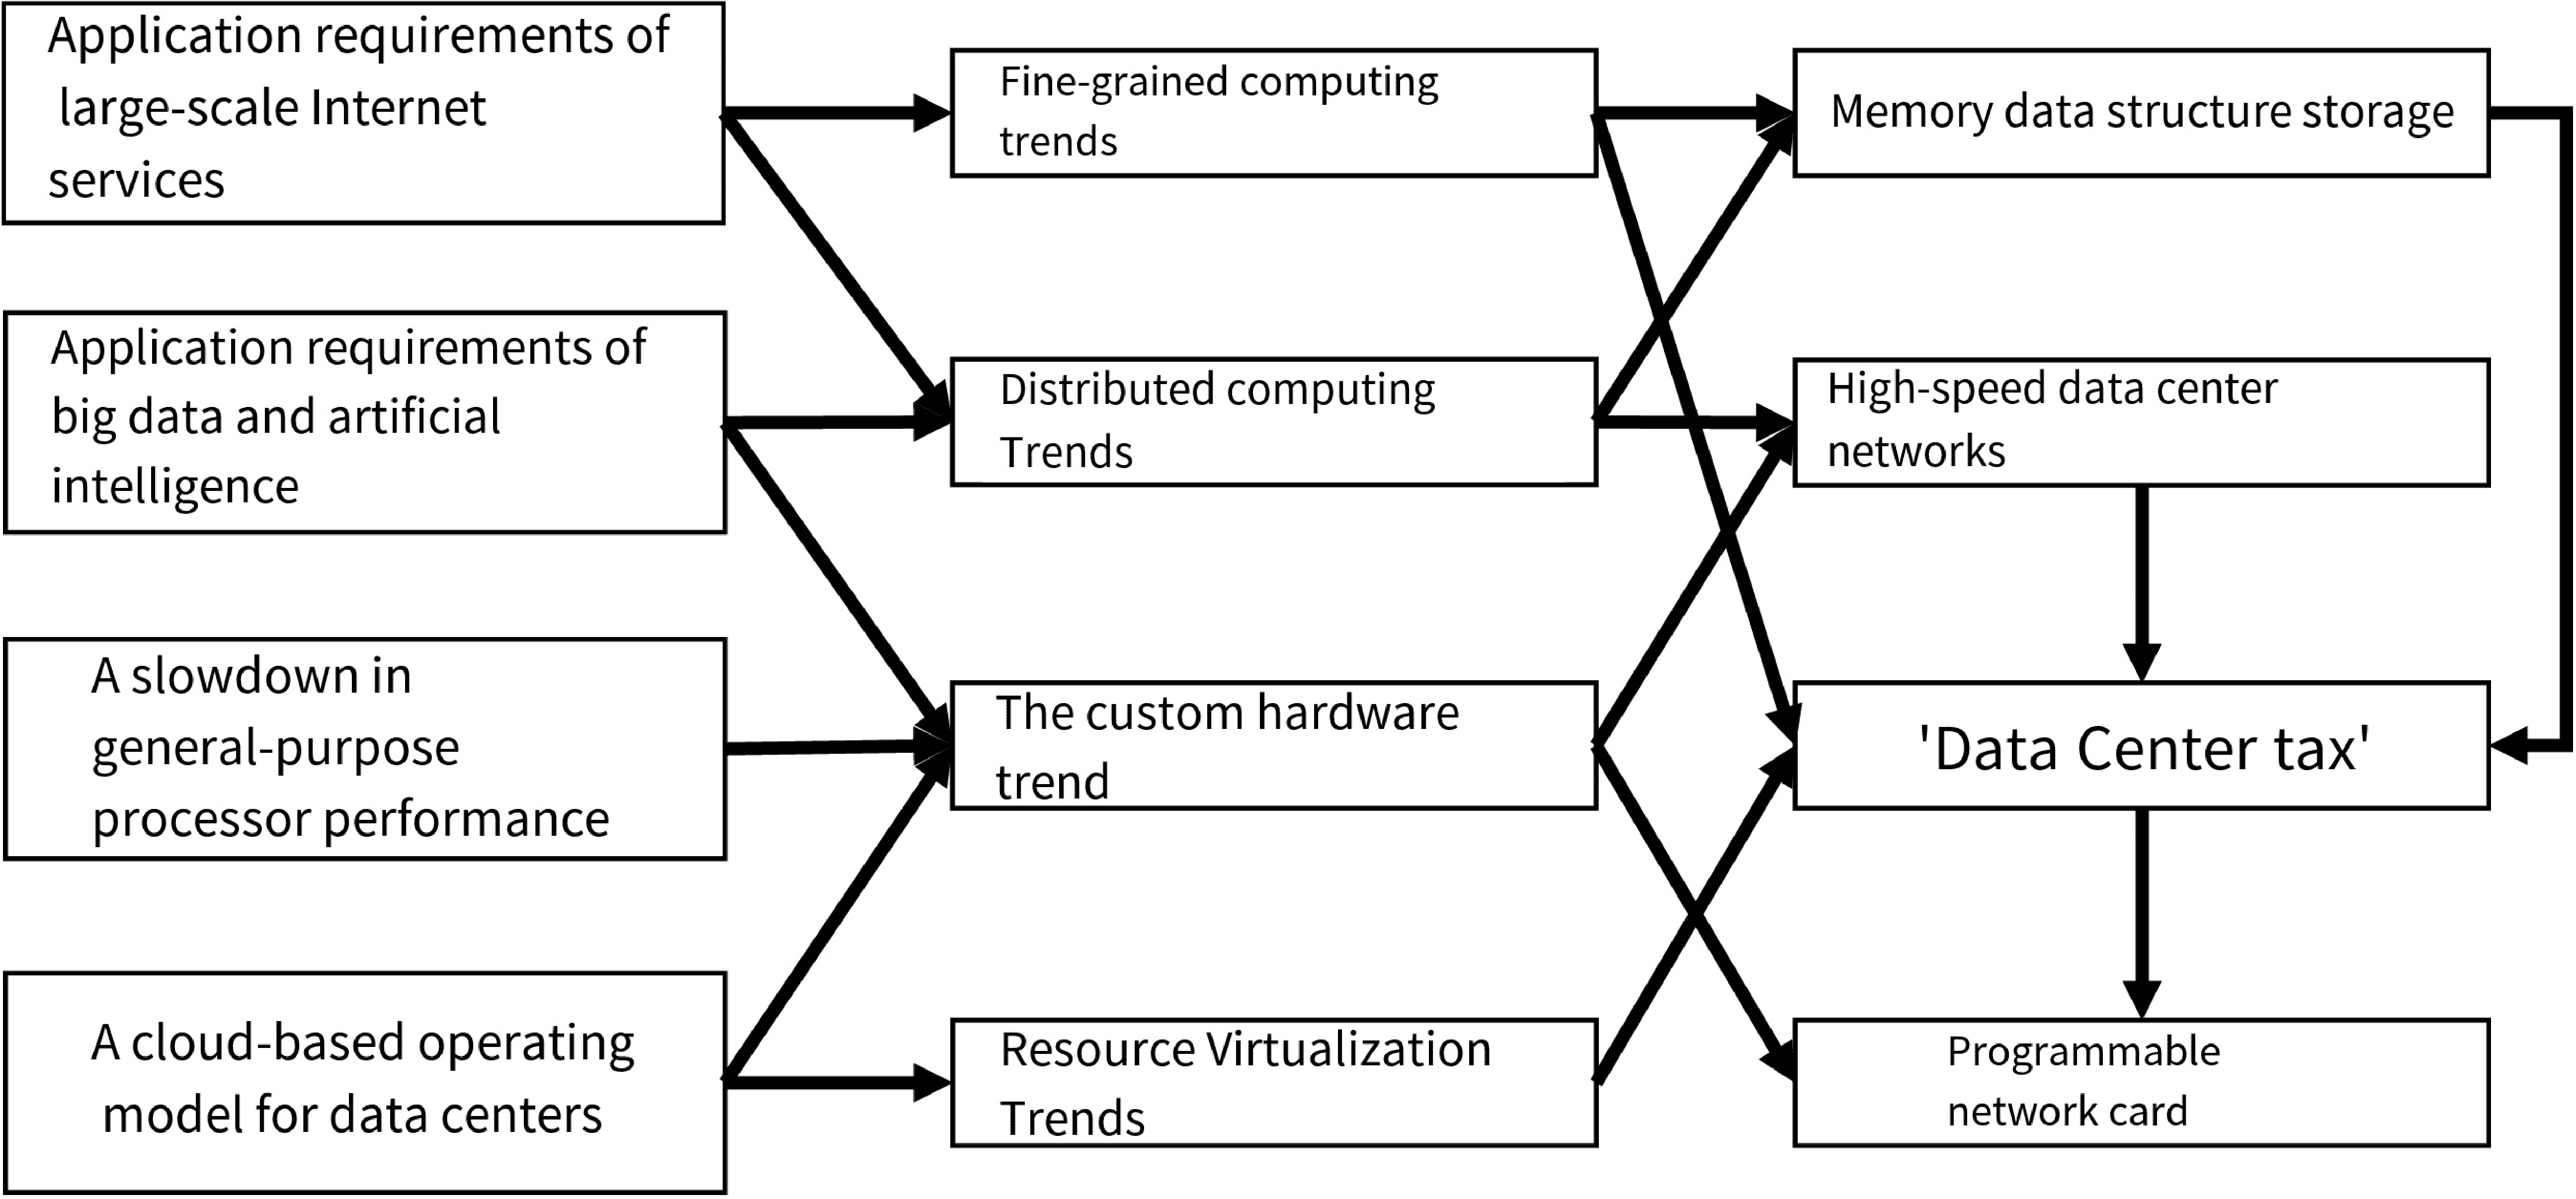
\includegraphics[width=0.9\textwidth]{figures/background_overview.pdf}
	\caption{Logical structure of this chapter.}
	\label{background:fig:overview}
\end{figure}

\section{Development Trends of Data Centers}
\label{background:sec:trend}

The history of data centers can be traced back to the computer rooms of early computers in the 1940s. Early computers were large precision instruments with high environmental requirements, requiring professional maintenance, and often running confidential military tasks, so they needed strictly controlled data centers for protection. With the development of computer technology, more and more users and businesses need to use computers. Since early computers were still very expensive, a company or research institution often had only a few computers, and users connected to the computers in the data center through terminals, forming the prototype of the client-server architecture.

From the 1980s to the 1990s, the evolution of hardware, guided by Moore's Law, and advancements in operating system software, spurred the robust development of personal computers (PCs). These PCs, while more affordable, had lower computing and storage capabilities and less stability. Concurrently, mainframes and minicomputers, which were derivatives of early computers, remained the preferred choice for businesses due to their superior computing and storage capabilities, higher stability, albeit at a higher cost. These costly mainframes required dedicated data centers and professional maintenance.

As the 20th century drew to a close, the rapid expansion of the Internet, coupled with its "free" business model and the swift increase in data volume and user numbers, rendered traditional mainframes and minicomputers too expensive and inflexible to accommodate rapidly expanding businesses. Consequently, an increasing number of Internet companies began to utilize standard servers, similar in structure to PCs, to establish Internet services, thereby creating distributed systems. The proliferation of standard servers led to the continuous expansion of data centers. These servers necessitated ample room space, high-speed and stable Internet connections, stable temperature and humidity, and cheaper electricity to minimize energy costs. As a result, the construction of data centers gradually became a specialized industry, and the term "data center" became standardized.

Around 2010, as Internet companies sprouted rapidly, there was a growing demand for highly scalable computing, storage, and network resources. Cloud computing, which offers on-demand rental of computing, storage, and network resources, emerged as an increasingly popular business model. More and more businesses began migrating their traditional IT systems to cloud computing platforms to reduce operation and maintenance costs. Compared to Internet data centers, cloud data centers offer a wider range of application types and user interaction methods, higher network interconnection performance, more customized hardware, and better resource reuse. The following four sections will discuss the four development trends of cloud data centers: resource virtualization, distributed computing, customized computing, and fine-grained computing.

\subsection{Resource Virtualization}
\label{background:sec:datacenter-virtualization}

Early computers and mainframes were costly. To allow multiple tasks to fully utilize computing and storage resources, the concept of virtualization was introduced. The time-sharing systems of the 1950s and 1960s \cite{strachey1959time,amdahl1964architecture} implemented the time-sharing reuse of hardware by multiple user tasks, evolving into the precursors of modern operating systems such as UNIX in the 1970s \cite{bach1986design}. From the 1970s to the 1990s, Virtual Machine Monitors (VMMs, or hypervisors) further implemented the time-sharing reuse of hardware by multiple operating systems \cite{popek1974formal,agesen2010evolution}, laying the technical groundwork for the development of cloud computing.

In the first decade of the 21st century, the development of the Internet led to an increasing number of companies needing to provide 24-hour network services, and Internet Data Center (IDC) hosting services gradually emerged. However, IDC hosting requires customers to purchase server hardware in advance and requires maintenance by operations personnel, resulting in high capital expenditure (capex) and operational expenditure (opex). Many companies' network services have high seasonality (such as Amazon's Black Friday promotion), so a large amount of computing resources are idle during off-peak times. On the other hand, the rapid expansion of data and user scale puts time pressure on hardware purchasing and IDC site selection. To this end, virtual machine hosting services provide on-demand virtual machine resources, enabling the slicing of server resources by CPU cores and time-sharing reuse among different customers, and facilitating management and scheduling by internal operations personnel.

Cloud computing is an upgraded version of virtual machine hosting services, with the hallmark change being the decoupling of computing and storage. Virtual host hosting services slice the computing and storage resources on a host into multiple virtual machines. If the host's hardware or virtualization software (hypervisor) fails, the virtual machine also shuts down, and there is a risk of data loss. In cloud computing, the storage resources of virtual machines have multiple replicas in distributed storage systems, so when a computing node fails, the virtual machine can be restarted from other computing nodes, and the failure of storage nodes is generally transparent to customers. The decoupling of computing and storage not only greatly improves service availability and data security, but also facilitates the upgrading of virtualization software and hot migration of virtual machines.

In addition to sharing hardware resources with other companies, IT companies utilize cloud computing for virtualization for another purpose, specifically to repurpose hardware infrastructure to provide different quality of service guarantees for various types of services within the company. For instance, web front-end servers responding to user requests, online transaction processing (OLTP) databases, online machine learning inference, and so forth, typically require lower latency; offline data processing (OLAP), data mining, distributed machine learning training, and so on, need to access massive data, perform a large amount of computation, and require higher throughput. Low latency and high throughput are somewhat contradictory \footnote{Latency refers to the time difference between the end of processing and the start of processing. Throughput refers to the number of requests processed per unit of time. Latency and throughput are two important indicators of system performance. Roughly speaking, throughput equals the number of parallel processing requests divided by the average latency.}, thus it is necessary to slice computing, network, storage, and other resources to provide different quality of service guarantees (Quality of Service, QoS) for applications with different needs.

As introduced in Section \ref{intro:sec:background}, the customer's virtual machines in a cloud data center are located on computing nodes, while storage services and network services run on decoupled storage and network nodes. In addition, management nodes are needed for scheduling and monitoring. As shown in Figure \ref{background:fig:cloud-architecture}, a data center is usually composed of computing, network, storage, management, and other nodes, as well as the interconnection network between nodes.

\begin{figure}[htbp]
	\centering
	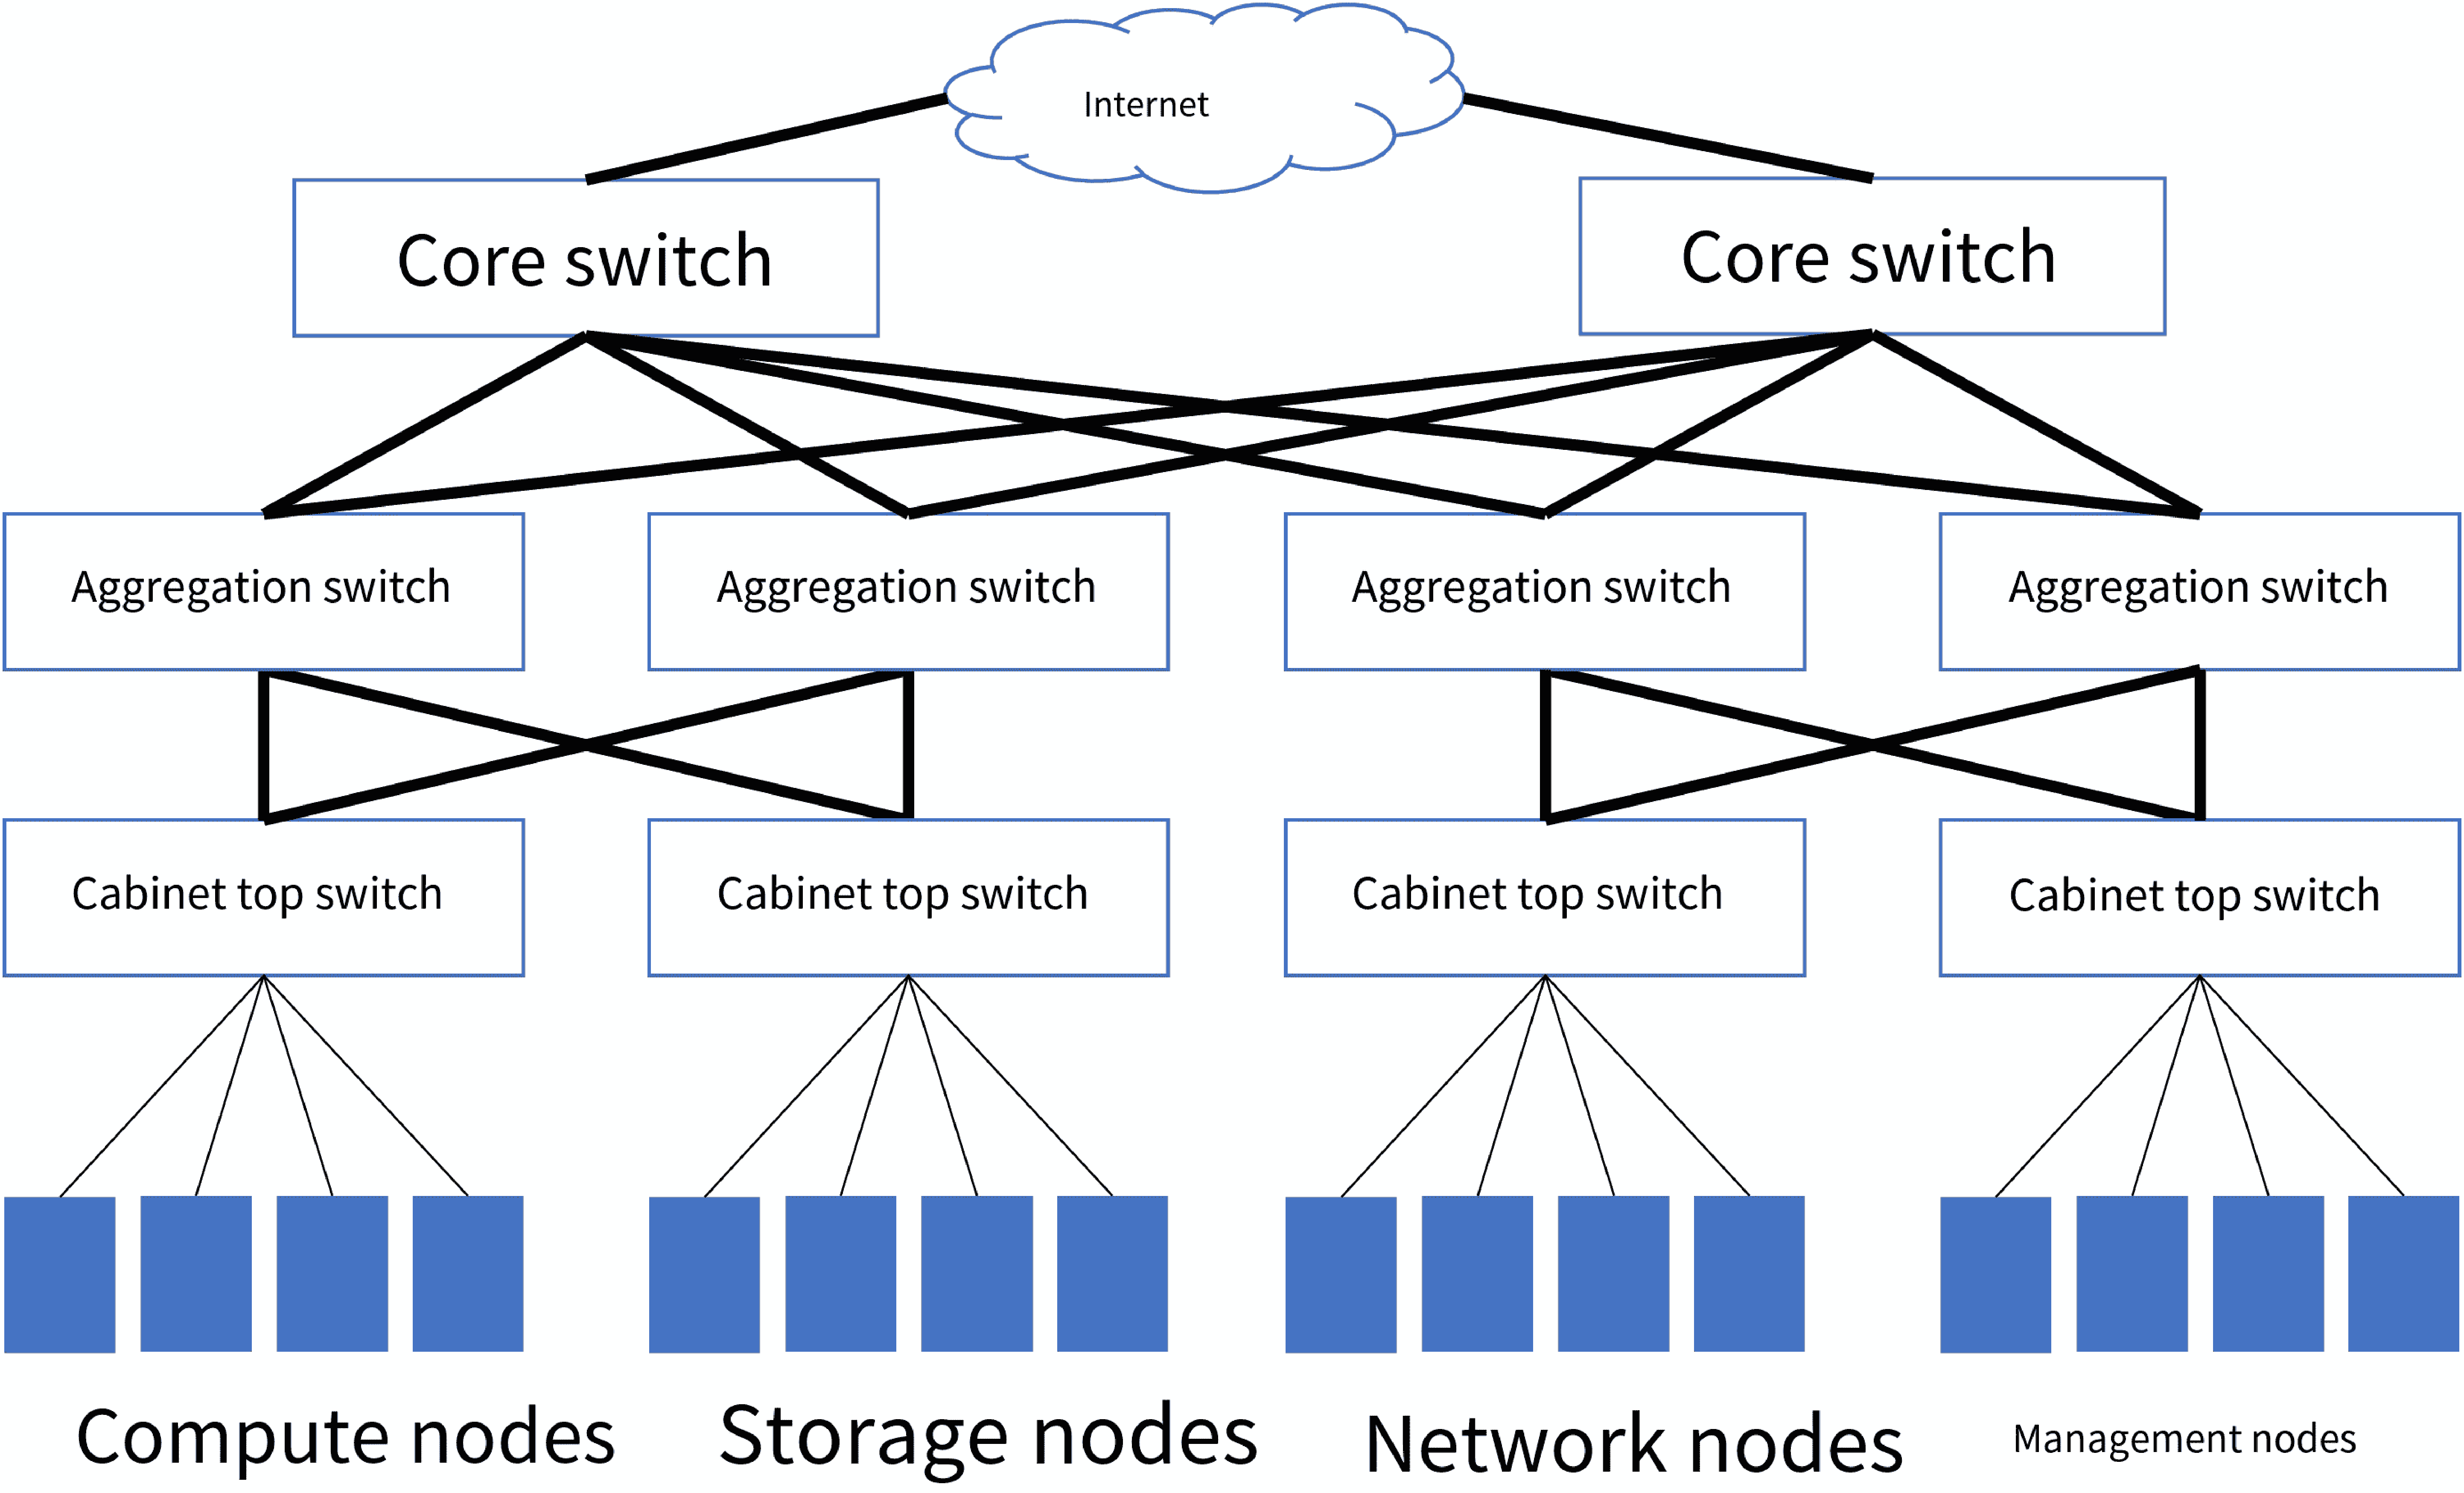
\includegraphics[width=0.6\textwidth]{figures/DC_arch.pdf}
	\caption{Data center architecture.}
	\label{background:fig:cloud-architecture}
\end{figure}

\subsection{Distributed Computing}
\label{background:sec:datacenter-distributed}

At the close of the 20th century, search engines bridging information islands signified the dawn of the Internet era. Search engines are required not only to gather, process, and index vast amounts of information, but also to respond to a high volume of user information retrieval requests in real time. Traditional mainframes and enterprise-level storage are not only expensive, but also incapable of meeting the scalability of massive information storage and user request processing \footnote{The scalability of a distributed system refers to the increase in system throughput with the number of nodes. Ideal scalability is a linear increase in throughput with the number of nodes.}. To address this, Google proposed the construction of scalable data centers using standard commercial servers, employing software to execute storage partitioning and redundancy, user request distribution, and to build fault-tolerant systems on relatively unreliable hardware foundations \cite{ghemawat2003google,chang2008bigtable,dean2008mapreduce}, thus spearheading the wave of large-scale distributed computing.

Workloads such as information retrieval and Web services are relatively straightforward to parallelize. There is virtually no correlation between each user request, hence they can be dispatched to different servers for parallel processing, and increasing the number of servers can almost achieve a linear increase in system throughput. Given appropriate indexing, the amount of data required to process each user request is also minimal, and there is no high demand for communication performance.

With the evolution of search advertising, social networks, and the mobile Internet, Internet companies have amassed vast amounts of user data. In order to extract knowledge from this massive data, big data began to emerge, giving rise to big data processing frameworks represented by Hadoop \cite{white2012hadoop} and Spark \cite{zaharia2010spark}. For instance, MapReduce \cite{dean2008mapreduce} borrowed the concepts of mapping and reduction from functional programming languages, and proposed a programming framework for large-scale data set parallel processing on unreliable hardware clusters.
Big data processing typically involves batch operations, requires access to massive data, and is not easy to parallelize and achieve linear acceleration.
The fundamental reason for the difficulty in parallelization is the communication overhead between nodes.
For example, in graph computing, the classic PageRank algorithm \cite{page1999pagerank} consists of several stages. In each stage, each node needs to update its weight based on the weight of its adjacent nodes. In distributed computing, each node processes a part of the node set, so each stage requires a large amount of communication between nodes.

The MapReduce intermediate results are stored on disk, which results in high I/O overhead. To address this, the Spark \cite{zaharia2010spark} big data processing framework suggests maintaining the intermediate calculation state in memory. In-memory computing has emerged as a new paradigm for big data processing \cite{ousterhout2010case,dragojevic2014farm}. Once the disk bottleneck is eliminated, the latency and throughput of the data center network become the new bottleneck of the distributed system. This has led to a performance leap in data center networks from 1 Gbps to 40 to 100 Gbps over the past decade \cite{al2008scalable} (as shown in Figure \ref{background:fig:network-perf-trend}), and the large-scale deployment of high-performance data center network transmission technologies represented by RDMA \cite{guo2016rdma}.

\begin{figure}[htbp]
	\centering
	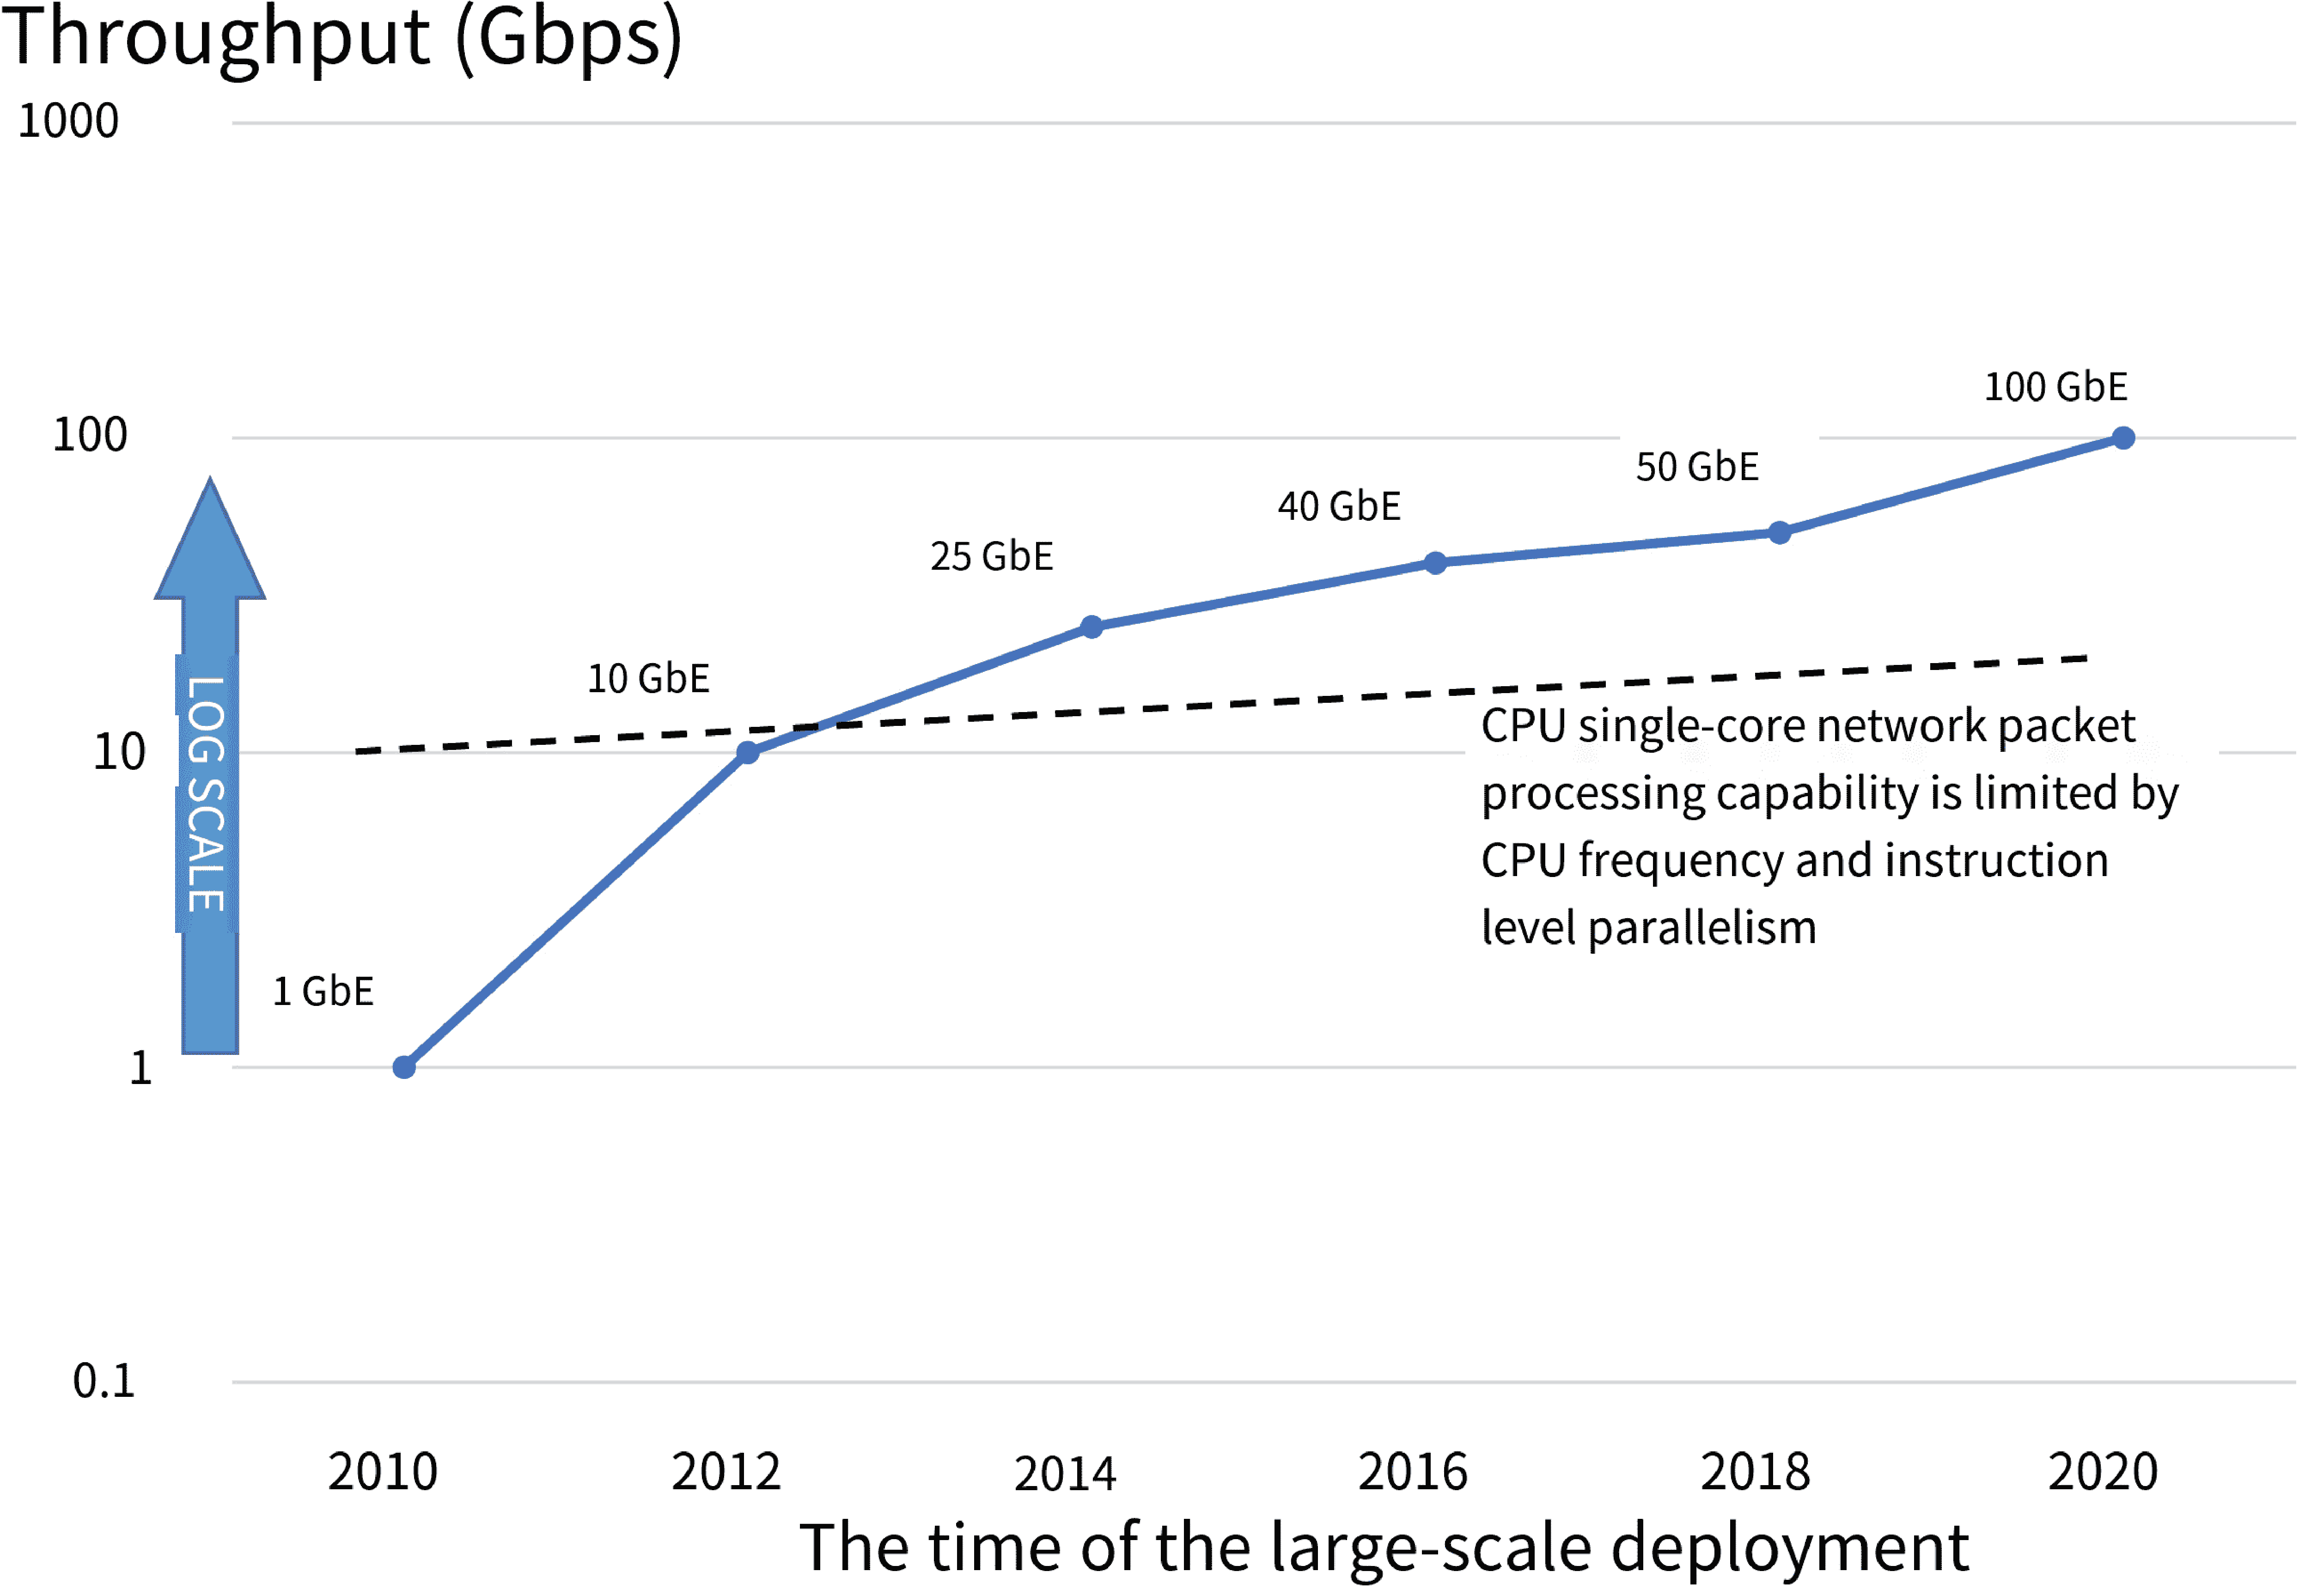
\includegraphics[width=0.6\textwidth]{figures/network_perf_trend.pdf}
	\caption{Rapid improvement of data center network performance.}
	\label{background:fig:network-perf-trend}
\end{figure}

In recent years, in-memory computing based on RDMA has significantly improved the performance of many distributed systems, including key-value storage \cite{dragojevic2014farm}, distributed transactions \cite{wei2015fast,chen2016fast,wei2018deconstructing}, remote procedure calls \cite{kalia2016fasst}, graph computing \cite{wang2018fast}, and more. However, having high-performance network hardware does not necessarily lead to improved communication performance in distributed systems. Section \ref{background:sec:datacenter-tax} of this article discusses how the "data center tax" of traditional operating systems makes it challenging for distributed applications to fully utilize the high performance of data center network hardware.

There are two paradigms for inter-process communication in distributed systems: message passing and shared memory \cite{kshemkalyani2011distributed}. In the message passing paradigm, the process serializes the data structure to be sent into a string and sends it to another process through a network message. Message passing in distributed systems typically adopts the remote procedure call (RPC) or message queue model, or a combination of the two. In the RPC model, the server side registers a procedure to respond to the client's RPC request. In the message queue model, the producer broadcasts or distributes messages to several consumers. To achieve decoupling of producers and consumers, buffering, and reliable delivery of messages, the message queue model often introduces a broker service, such as Kafka \cite{kreps2011kafka}. In terms of programming interfaces, distributed applications usually use RPC libraries and message queue middleware, which rely on the socket interface of the operating system to send and receive messages.

In the shared memory paradigm, multiple processes share memory space, and the content written by one process can be read by all processes. Remote Direct Memory Access (RDMA) technology aims to provide a shared memory abstraction for distributed systems. It has been deployed in more and more data centers in recent years and is a hot research topic in the system academic community. However, in many cases, the abstraction level of shared memory is too low. Applications need to manage memory allocation and release and object layout in memory on their own. Synchronization between processes is also required when multiple processes write at the same time. On the other hand, the abstraction level of traditional relational databases is too high, too heavyweight, and performance is limited. The abstraction level of shared data structures is between shared memory and relational databases, and it can efficiently and flexibly store structured and semi-structured data. A typical example of shared data structure storage is Redis \cite{redis}, whose basic abstraction is a key-value mapping table. Users can specify a key to get or modify the corresponding value. The value can be a simple string or a more complex data structure, such as a list, set, priority queue, dictionary, etc. Redis also provides operation primitives for these data structures. Since key-value mapping is a commonly used basic data structure, many data structure storages are also called key-value storages. Shared data structure storage can reside in memory or be persisted to disk or flash.

Memory shared data structure storage is increasingly the choice of distributed applications.
For example, the Spark \cite{zaharia2010spark} big data processing framework uses Resilient Distributed Datasets (RDD) as the basic abstraction, abstracting big data processing into a data flow graph. Each node in the graph reads data from the RDD, performs transformations, and outputs the results to the RDD. Because RDD storage can achieve high availability and scalability, big data processing programs written with RDD abstraction also have fault tolerance \footnote{In distributed systems, resilience refers to the ability of the system to automatically recover and continue running using the remaining nodes when a node experiences unpredictable hardware failures or operating system crashes.} and scalability.

Message passing and shared data structure are two paradigms of inter-process communication, each with its own advantages and disadvantages in different scenarios. Both are crucial for the performance of distributed systems. These two communication paradigms can not only be theoretically converted to each other \cite{attiya1995sharing}, but also often switch to the other paradigm in implementation. For instance, RDMA shared memory and distributed data structure storage send read and write requests and data via network messages; FaSST \cite{kalia2016fasst} implements high-performance RPC through RDMA shared memory read and write primitives; Redis \cite{redis} key-value storage system can function as a lightweight message queue service. Chapters \ref{chapter:clicknp} and \ref{chapter:socksdirect} of this paper are dedicated to enhancing the performance of message passing. Chapter \ref{chapter:kvdirect} of this paper is dedicated to enhancing the performance of memory shared data structure storage.

Since 2012, neural networks have been revived, deep learning has emerged as a new paradigm in machine learning, and artificial intelligence has entered another peak that continues to this day.
It is widely recognized that data and computing power are the two main drivers of the revival of deep learning, with the computing power primarily supplied by customized hardware GPUs different from CPUs.
The advancement of deep learning demands increasingly high computing power, which in turn stimulates the development of GPUs and various deep learning processors.
Because the computing power of a single machine is insufficient to train large models on big data, distributed machine learning training has become mainstream.
Distributed machine learning training typically employs the Stochastic Gradient Descent (SGD) method. SGD consists of several stages (epochs). At the start of each stage, all computing nodes share a model, use different training data to calculate the gradient of the model, then aggregate the model gradients of all computing nodes, modify the model, and use it as the shared model of all computing nodes in the next stage.
Distributed machine learning training primarily has three architectures: Iterative MapReduce (IMR), parameter server, and data flow \cite{distributed-ml}.
Iterative MapReduce utilizes the infrastructure of big data processing platforms and is suitable for data parallelism \footnote{Data parallelism in machine learning refers to different nodes using different data for training. Note the difference from data parallelism within FPGA mentioned later.} and synchronous communication.

The issue with synchronous communication is that the performance of the entire system is hindered by the slowest node, and if one node fails, the entire system cannot continue to operate. As a result, asynchronous Stochastic Gradient Descent and semi-synchronous Stochastic Gradient Descent training methods have gained popularity in recent years. In asynchronous communication methods, each node continues to train on local data, but does not need to wait for other nodes to finish training before distributing local model gradient updates to all other nodes. To facilitate the distribution of models and the aggregation of model gradients, distributed machine learning training systems often equip a distributed parameter server \cite{li2014scaling}. Each worker node retrieves the current parameters from the parameter server and uploads the local gradient updates to the parameter server. A distributed parameter server not only balances the load of each parameter storage node but also reduces communication overhead when worker nodes only access part of the parameters.

The parameter server architecture can support not only data parallelism but also model parallelism \footnote{Model parallelism in machine learning refers to multiple nodes calculating part of the model, i.e., the gradient of a training data needs to go through multiple nodes to be calculated.}. For instance, DistBelief \cite{dean2012large} utilizes both data parallelism and model parallelism; AlexNet \cite{krizhevsky2012imagenet} leverages the independence of computations between layers in convolutional neural networks and employs model parallelism. The parameter server is a typical application of key-value storage. Taking Microsoft's Multiverso parameter server \cite{multiverso} as an example, parameters can be vectors, matrices, tensors, hash tables, or sparse matrices. At present, most distributed machine learning systems of large internet companies use the parameter server architecture.

Owing to the growing popularity of data and model hybrid parallel distributed machine learning training methods, distributed deep learning systems based on data flow, such as Tensorflow \cite{abadi2016tensorflow}, have emerged in recent years. In data flow systems, each node in the data flow graph represents a data processing operator, which is a finite state automaton. Nodes are connected by control message flows and data flows, adopting the distributed system communication paradigm of message passing. In fact, nodes in the data flow graph can also be parameter servers, which transforms into the distributed communication paradigm of shared data structures.

\subsection{Customized Hardware}
\label{background:sec:datacenter-customized}

In the era of mainframes, mainframes and even supercomputers that needed to process a large amount of information generally adopted integrated hardware and software systems, that is, the hardware and software were developed by the same company team. Due to the use of high-speed hardware interconnection and hardware redundancy, these systems often have both high performance and high reliability, but the cost increases sharply with the expansion of the system scale.

As mentioned in Section \ref{background:sec:datacenter-distributed}, since the end of the 20th century, Internet data centers are usually composed of standard commercial servers. The reason why these ordinary commercial servers are low in cost is because their architecture is similar to a large number of commercial personal computers (PCs), and the components such as CPU, memory, motherboard, hard disk, and network card are all standard components, independently designed and implemented by various professional companies. The operating system, database, web server and other software are also standardized, either developed by professional companies or open source software. Standard components with large production volumes can better amortize one-time engineering costs such as research and development and wafer production, thereby reducing the price of standard components. Although the system composed of standard components reduces the hardware and software costs of the data center, it also imposes restrictions on the developers of standard components: everyone needs to comply with the interfaces and protocols between standard components and can only innovate within their own boundaries. The builders of the data center system can only combine standard components like building blocks, and it is difficult to consider and optimize globally.

Since 2010, the trend of cloud computing scale, the demand of data center applications, and the performance limitations of general-purpose processors have made customized computing a trend in data centers, and engineers have regained the opportunity for hardware and software co-design. First, in the cloud computing platform, the software and hardware environment are controlled by the service provider. After reaching a certain scale, all forms of customization become possible. As long as it can improve performance, reduce prices, and enhance competitiveness, cloud service providers have enough motivation to customize chips, change network protocols, change server architectures, modify operating systems, and even rewrite applications. Secondly, as mentioned in Section \ref{background:sec:datacenter-distributed}, applications such as big data and machine learning have a high demand for computing power. Finally, the performance limitation of general-purpose processors is the main driving force for customized hardware, which will be discussed in detail below.

Moore's Law predicts that the performance of unit area integrated circuits can be improved by making the storage and processing units smaller and smaller, thereby increasing the number of storage and processing units of unit area integrated circuits. More profound is Dennard's scaling law \cite{dennard1974design}, that is, the performance of integrated circuits can double every two years without consuming more energy and area. Its theoretical basis is that a new generation of semiconductor technology is adopted every two years, the transistor size is reduced by 30%, and the chip area is reduced by 50%. In order to maintain a constant electric field, the voltage is reduced by 30% in proportion to the transistor size. At the same time, because the chip size is reduced, the delay is reduced by 30%, and the clock frequency can be increased by 40% \cite{borkar1999design,borkar2011future}. In that era, the dynamic power consumption of integrated circuits accounted for the main part of power consumption, which was directly proportional to capacitance, the square of voltage, and frequency, so it can be calculated that power consumption is reduced by 50%. According to this ideal model, the area and power consumption of integrated circuits are halved every two years, so twice the number of transistors can be stuffed under the original area and power consumption, and the clock frequency is also increased to 1.4 times. For the single-threaded microprocessor of the von Neumann architecture, these additional transistors are mainly used for larger caches, more complex pipelines, superscalar, out-of-order execution, register renaming, branch prediction, etc., to increase the number of instructions that can be executed per clock cycle. According to Pollard's empirical law \cite{pollackpollack}, the computing power per clock cycle is roughly proportional to the square root of the number of transistors. The computing power per unit time is equal to the clock frequency multiplied by the computing power per clock cycle, so the performance of the microprocessor is doubled every two years without consuming more energy and area.

Regrettably, since the advent of the 21st century, the dividends of Moore's Law and Dennard's scaling law have been gradually diminishing. Firstly, as the feature size of integrated circuits reduces, the voltage also decreases. However, the lower the threshold voltage that controls the transistor, the faster the leakage current of the transistor will increase, becoming a significant part of the power consumption of integrated circuits. To control the leakage current, the threshold voltage cannot be reduced, and may even need to be higher than the previous generation of integrated circuits \cite{borkar1999design}. Therefore, for each new generation of semiconductor technology, the power consumption of each transistor will not be halved as anticipated. 

Secondly, because the area of each transistor is halved and the power consumption is not reduced proportionately, the power consumption of unit area integrated circuits will increase. The heat dissipation problem of the chip has become a major factor limiting the scale of integrated circuits \cite{borkar2011future}. 

Furthermore, for the same integrated circuit, within the permissible range, in order to double the performance and double the clock frequency, the voltage must be doubled accordingly to reduce the flip delay of the transistor. Thus, the power consumption is roughly proportional to the cube of the clock frequency. Due to the limitation of heat dissipation, the clock frequency of integrated circuits is also limited, and it is unrealistic to significantly improve the performance of integrated circuits by "overclocking". 

Lastly, the 7 nm semiconductor process has been mass-produced, and the radius of a silicon atom is 0.1 nm. As the feature size of integrated circuits is getting closer and closer to the atomic size, quantum effects cannot be ignored, which brings significant technical challenges to lithography technology \cite{borkar2011future}. In fact, since around 2010, the shrinkage of the feature size of integrated circuits has significantly slowed down and can no longer maintain the speed of one generation every two years. 

In conclusion, under the current semiconductor technology framework, the performance of unit area integrated circuits can no longer maintain the speed of doubling every two years, and the improvement of performance also means the increase of power consumption, and the "free lunch" is over.

However, from the standpoint of chip architecture, the traditional von Neumann architecture is unable to fully exploit the computational capacity of each transistor. Consequently, there remains an opportunity to "extract as much as possible from this lemon that is Moore's Law" \cite{threebody}. Theoretically, the computational power per clock cycle could be proportional to the number of transistors, but the aforementioned Pollack's empirical law \cite{pollackpollack} suggests that the computational power per clock cycle of von Neumann microprocessors is empirically proportional to the square root of the number of transistors. For instance, the world's first microprocessor, Intel 4004, manufactured in 1971, utilized a 10-micron process, contained 2300 transistors, had a clock frequency of 108 KHz, and could execute 90 K 4-bit operations per second. The Intel Xeon E5 microprocessor, based on the Broadwell architecture in 2016, utilized a 14-nanometer process (1 M times that of 4004), contained 7.2 billion transistors (3 M times that of 4004), had a base frequency of 2.2 GHz (20 K times that of 4004), and could execute approximately 300 G 64-bit operations per second \footnote{Assuming the application uses AVX2 instructions, does not use FMA3 instructions, and does not overclock.} (3 M times that of 4004) \cite{intel-e5-v4}. As can be observed, the number of operations that Xeon E5 can execute per clock cycle is approximately 150 times that of 4004, while the number of transistors is 3 million times. Even when considering the complexity of 64-bit computing compared to 4-bit computing, it still implies that the contribution of each transistor in 4004 to computational power is hundreds of times higher than that of Xeon E5. This is because the instruction set and microarchitecture of von Neumann microprocessors are becoming increasingly complex, firstly to enhance single-thread performance, secondly to add deeper cache levels to address the "memory wall" issue, and thirdly to support communication and synchronization between cores, operating systems, and virtualization technologies. The proportion of transistors actually used for computation is diminishing progressively.

Due to the performance bottleneck of von Neumann architecture processors, customized hardware has emerged as a trend. The basic operations of customized hardware do not need to be expressed through instructions, and the data operation process is relatively fixed, eliminating the need for overhead related to von Neumann architecture, instruction decoding execution, and pipeline control. Customized hardware can customize data paths and memory levels, circumventing the "memory wall" problem of von Neumann architecture where all memory addresses share access. Customized hardware can construct numerous processing units to parallel process the same type of data (such as matrix operations), or a deep pipeline to process deep logic level calculations (such as symmetric encryption). As depicted in Figure \ref{background:fig:moores_law_redefined}, the energy efficiency of Nvidia GPUs such as K80, P100, P40, V100, Intel FPGAs such as Arria 10, Stratix 10, and Google's deep learning processor TPU is significantly higher than that of general-purpose processors (note that the y-axis is a logarithmic coordinate system), and essentially follows Moore's Law's prediction in terms of performance, that is, the energy efficiency of customized hardware doubles every 18 months.

\begin{figure}[htbp]
	\centering
	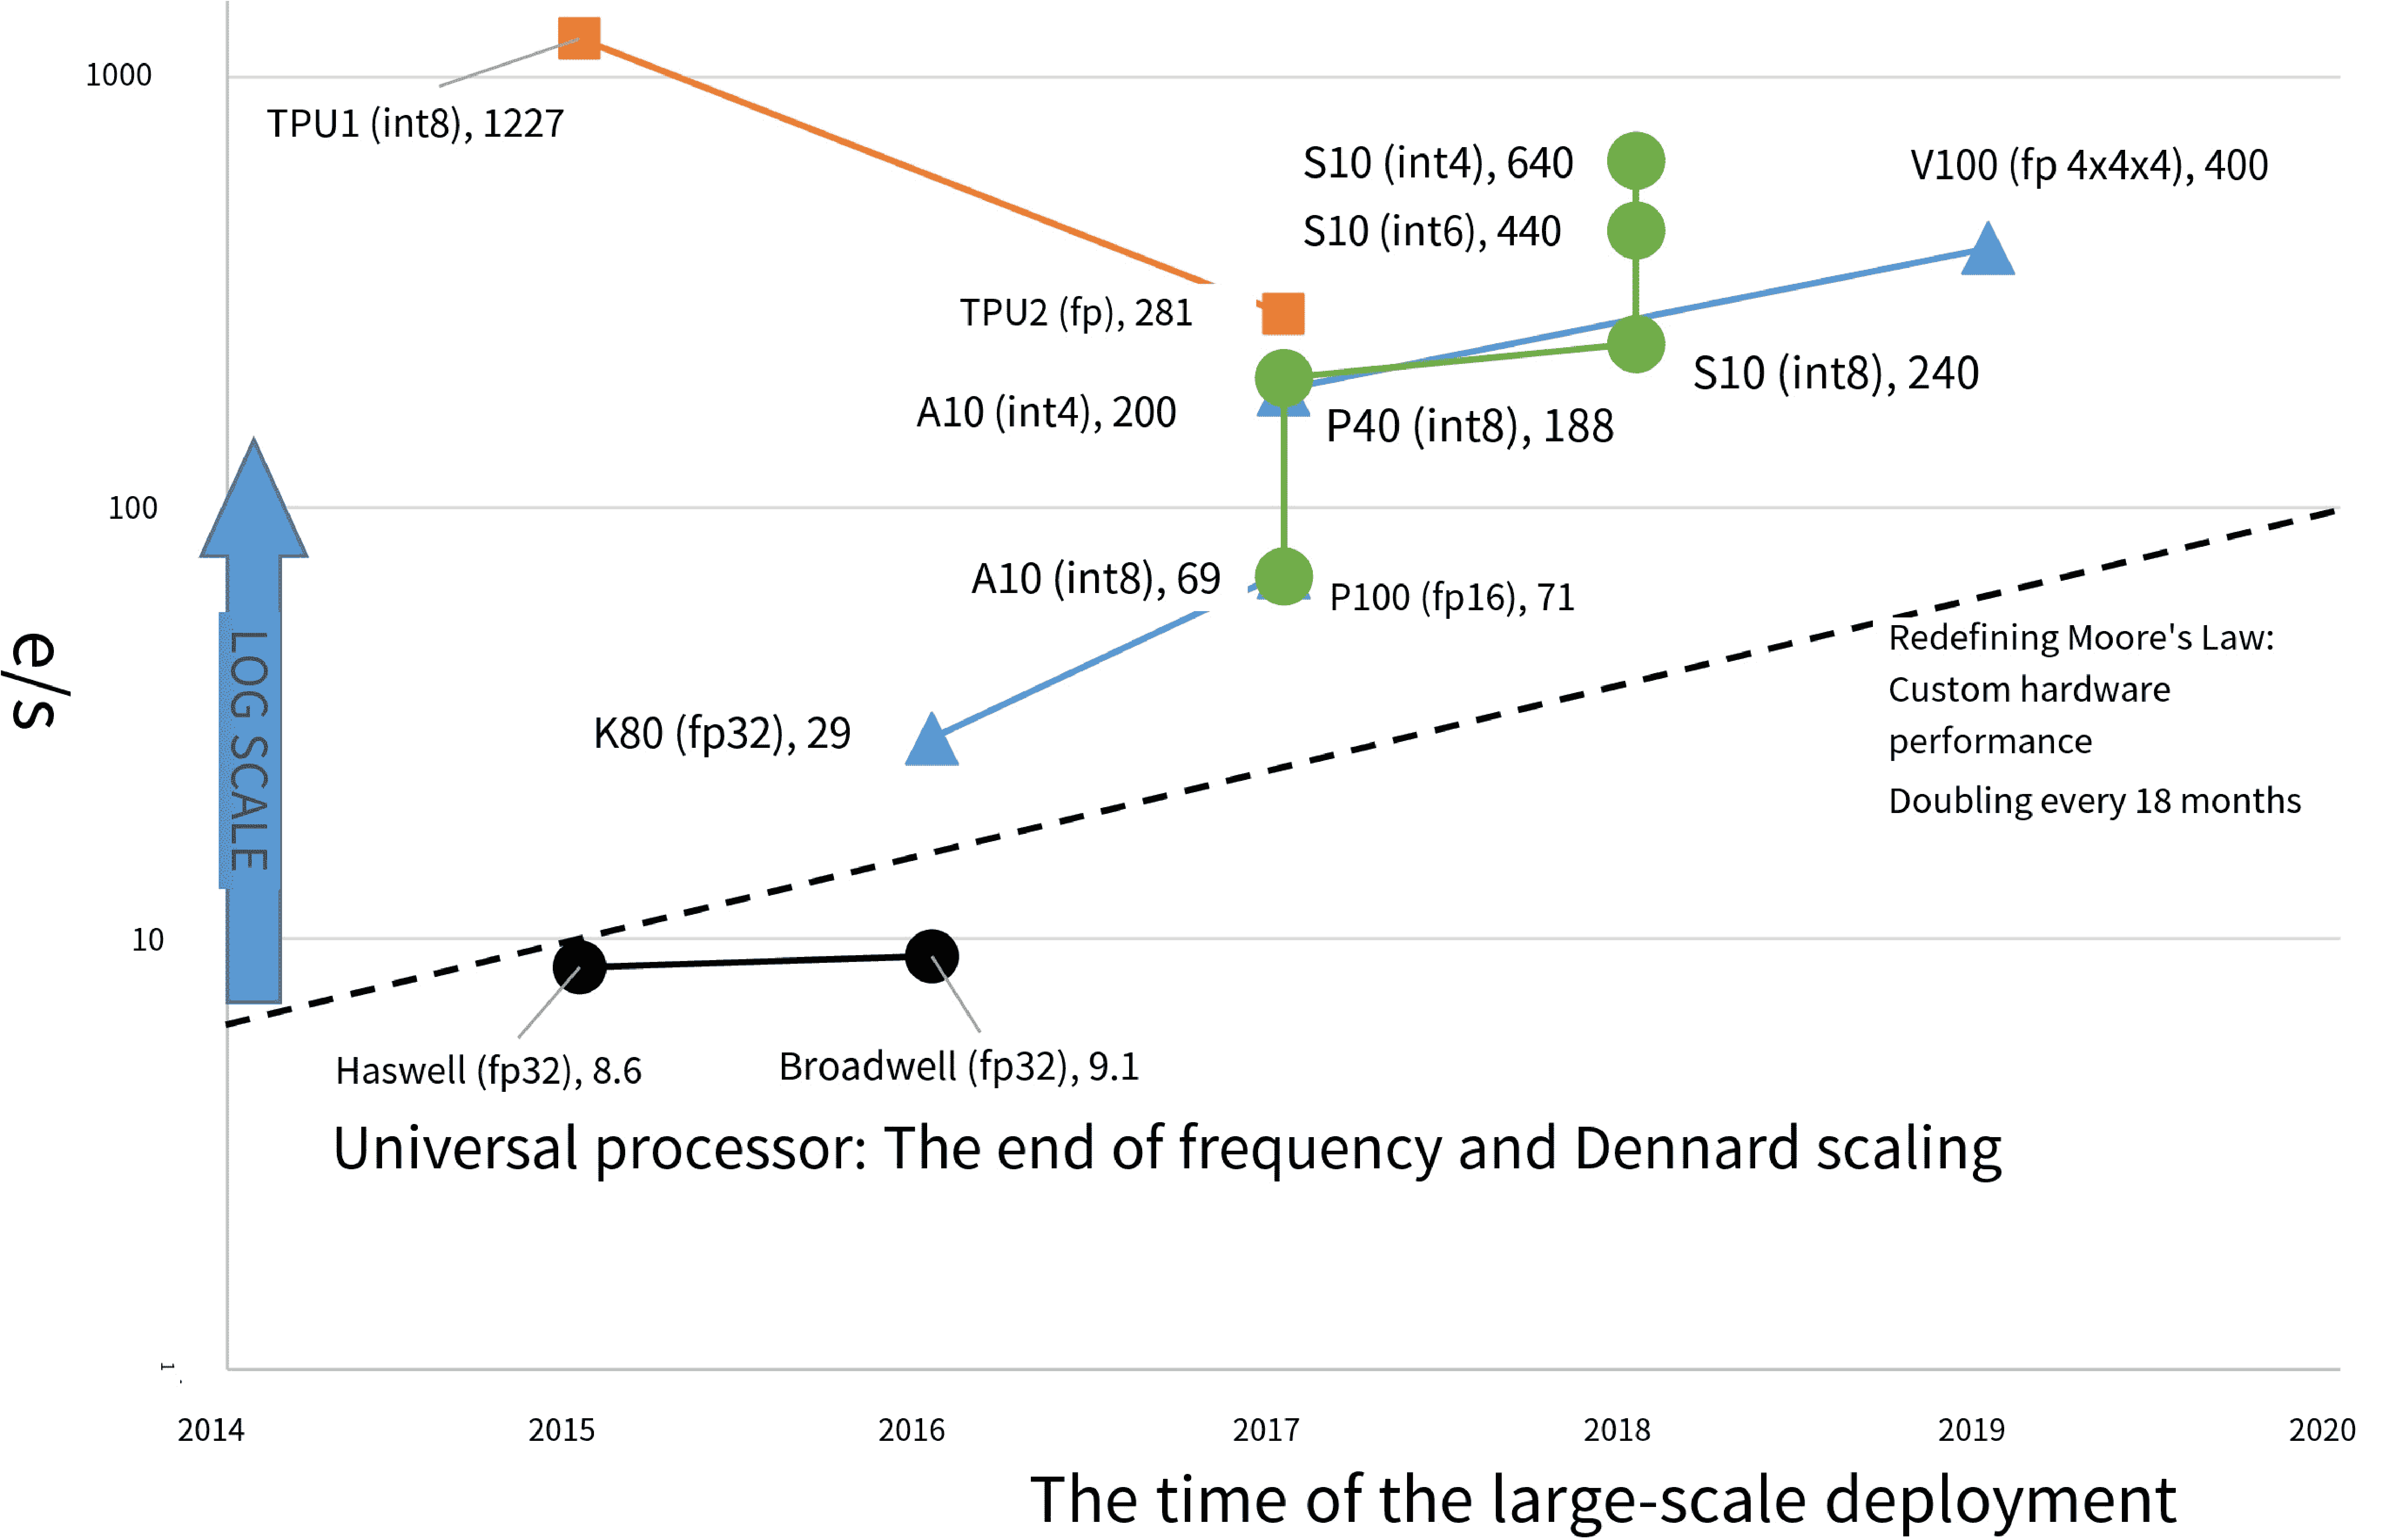
\includegraphics[width=0.8\textwidth]{figures/moores_law_redefined.pdf}
	\caption{The frequency of general-purpose processors and Dennard scaling gradually end, but customized hardware redefines and continues Moore's Law.}
	\label{background:fig:moores_law_redefined}
\end{figure}

\subsection{Fine-grained Computing}
\label{background:sec:datacenter-granular}

Since the introduction of the Docker framework in 2013, numerous Internet companies have utilized containers to deploy services \cite{bernstein2014containers}. Containers are not merely lightweight virtual machines, but more importantly, they redefine the architecture of Internet services, decomposing a few complex macroservices into a large number of simple microservices. Each microservice is deployed in the form of a container, enabling efficient scalable data center scheduling, software dependency management, and isolation between microservices, enhancing the efficiency of development, testing, and operation. The computing granularity of the microservice architecture is finer than the traditional architecture, hence the demand for total request service capability is higher, and the demand for communication between microservices is also high. For instance, WeChat operates more than 3000 microservices on over 20,000 servers. The entrance layer microservices respond to 10 billion to 100 billion user requests per day, and each user request triggers more microservice requests within the system, so the entire WeChat backend needs to respond to hundreds of millions of microservice requests per second \cite{zhou2018overload}.

Containers represent a more refined computing paradigm than virtual machines. A single server host can deploy hundreds of containers, while typically only dozens of virtual machines can be deployed. 

Firstly, the need to support a larger number of containers presents challenges for data center virtualization. In terms of computing virtualization, traditional virtual machines generally allocate CPU cores directly to the virtual machine. However, the number of containers usually exceeds the number of CPU cores, necessitating the operating system to schedule and allow various containers to time-share CPU cores. This increases scheduling overhead and also complicates performance isolation and quality of service assurance. In terms of network and storage virtualization, the number of containers is an order of magnitude larger than that of virtual machines, exerting pressure on lookup table capacity, queue numbers, cache capacity, and so on.

Secondly, the division of macro services into microservices has led to an increase in communication between containers. Many communications that were originally within the same virtual machine have become communications between containers, putting pressure on the container network within the server. To prevent a significant decline in the performance of microservices, it is necessary to ensure that the performance of the server container network is close to the performance of shared memory communication.

Thirdly, to enhance the fault tolerance and scalability of microservices, stateless microservice design has gradually become a trend. This means that the container itself does not store state, input data, output data, container configuration, and internal state are all stored in the data structure storage service outside the container. This necessitates the data structure storage to have low latency, high throughput, and high availability.

Container-based microservices are not the endpoint of reducing computing granularity. Traditional operating system processes still run inside the container, and these processes consume a certain amount of memory resources even without external requests. To ensure that the container can respond to user requests that may come at any time, computing resources such as CPU also need to be reserved. Containers also need to occupy a certain amount of storage space. Therefore, cloud service providers need to reserve computing, memory, and storage resources for each container, and charge for these reserved resources. The scaling, scheduling, and operation and maintenance of containers also need to be borne by the users of the containers. Although there are open-source frameworks such as Kubernetes, it also increases the burden on container users. In 2015, Amazon AWS launched a serverless computing service called Lambda, which allows users to only write event-driven business code within the programming framework of the cloud service provider, and leave tasks such as execution environment, scaling, scheduling, etc. to the cloud service provider. At present, mainstream cloud service providers such as Amazon, Microsoft, Google, Alibaba, and Tencent all provide serverless computing services.

In 2019, the University of California, Berkeley's forecast report on serverless computing indicated that despite the numerous advantages of the serverless computing paradigm and its promotion by major cloud service providers, the performance and cost of many applications utilizing serverless computing are not ideal due to issues with cloud storage performance and the absence of temporary storage services. 
Indeed, serverless computing is not a novel concept. 
Current big data processing frameworks (such as Spark) and data lake services from cloud computing manufacturers are generally stateless for fault tolerance and scalability, and are widely adopting the serverless computing paradigm. 
Traditional machine learning frameworks often separate training and inference, while in reinforcement learning, the agent needs to constantly interact with the surrounding environment, and training and inference are constantly cycling, thus necessitating fine-grained computing. 
The distributed reinforcement learning framework Ray also employs a stateless data processing function programming model and saves the intermediate state of the data stream processing process through key-value storage.

In summary, fine-grained computing presents challenges to the performance of data center virtualization, container networks, data structure storage services, and operating system scheduling.

\subsubsection{Programmable Switches}

The trend towards programmable switches is driven by both demand and hardware. From the demand perspective, the automation of network operations (self-driving network) is becoming increasingly important. To achieve automated network fault detection, diagnosis, and recovery, intelligence must be incorporated into the network, rather than treating the network as a black box. For this reason, programmable packet capture and statistical functions need to be added to the switch. Moreover, by utilizing the high-speed packet processing capabilities of the switch, caching, aggregation, synchronization, transaction processing, etc., in distributed systems can be accelerated, and low-latency, lossless networks also require the support of programmable switch hardware. Many people believe that adding programmability to switches will increase chip area and power consumption, but this is not necessarily the case. Barefoot Company pointed out that about 30\% of the area of the switch chip is used for serial IO communication, 50\% of the area is used for memory for lookup tables and packet buffering, and only 20\% of the area is used for packet processing logic. As the bandwidth of the switch continues to grow, the chip area is also increasing, and at this time, the 20\% area used for packet processing has spare capacity, which can accommodate more logic \cite{barefoot-programmable}.

Programmable switches can be categorized into three levels based on their programmability, from low to high. The first level includes switches that adhere to the OpenFlow standard. The packet processing logic is a pipeline composed of several match-action tables, but each table has certain restrictions on matching and execution. The second level includes switches that adhere to the P4 standard. Based on the pipeline structure, the matching rules, operations to be performed, and packet header parsing rules for each table entry can be customized. The third level is network processors, which use multi-core CPUs specifically designed for network processing to process each packet. This level can achieve maximum flexibility, but the throughput of a single network connection is limited by the CPU frequency. In reality, fixed-function pipelines, general-purpose programmable pipelines, and network processors are not clearly distinguished. In data center switches, a trend towards gradual integration can be observed, such as using crossbar switches or on-chip networks to flexibly interconnect various packet processing modules and on-chip memory.

To simplify switch operation and maintenance, Microsoft initiated the SONiC white box switch open source project \cite{sonic}. Firstly, a set of switch chip APIs were defined, allowing the hardware and software of the switch to evolve independently without worrying about compatibility issues. Secondly, a container-based modular switch software architecture was designed. By storing persistent states independently of the container, fine-grained fault recovery and zero service interruption time online upgrades were achieved. Finally, monitoring and diagnostic capabilities were provided to support automatic network operation and maintenance.

\subsubsection{RDMA Network Cards}

Traditional Ethernet network cards have relatively simple functions. The network protocol stack is implemented in the operating system kernel, and software middleware provides higher-level abstractions such as RPC, message queues, etc., to the application program. In cloud computing scenarios, virtual switch software is also needed to implement network virtualization and firewall and other network functions. Therefore, the end-to-end round-trip latency of the data center network is as high as hundreds of microseconds on average, and in extreme cases, it can even reach the millisecond level, which cannot meet the needs of low-latency distributed computing. Among them, the latency of the software accounts for the main part. The Infiniband \cite{infiniband2000infiniband} network commonly used in high-performance computing implements most of the network protocol stack in the network card, which can achieve end-to-end microsecond-level latency, so the Remote Direct Memory Access (RDMA) technology in it has begun to become popular in data centers. To be compatible with existing data center networks, RDMA network cards in data centers usually use Ethernet and UDP/IP, and then encapsulate the RDMA reliable transmission protocol on top of it. However, the deployment of RDMA in cloud computing data centers is much more complicated than in high-performance computing: firstly, the scale of data centers is larger than that of high-performance computing clusters; virtual machines sharing the same physical host need isolation and QoS; virtual machines need hot migration and fault recovery capabilities; in addition, there are many types of applications in data centers, and communication patterns are complex, RDMA primitives have a low level of abstraction, and socket compatibility and higher-level abstractions such as RPC are needed.

\subsubsection{Low-latency Network Transmission Protocol}

The ideal network and interconnect should be capable of scaling to millions of devices and components within the data center, possess low latency, high bandwidth, and lossless characteristics, and be able to withstand the failure or even malicious attacks of some components. For this reason, network and interconnect designers can draw from a variety of historical designs, such as supercomputers, on-chip networks, interconnects between line cards in core routers, circuit-switched networks, time-division multiplexed networks, etc. On the other hand, they can utilize new physical layer technologies, such as optical switching chips, laser communication, and 60G wireless networks, etc.

The network latency from the sending network card to the receiving network card in the data center primarily includes the propagation delay on the optical fiber, the processing delay of the switch, and the queuing delay in the switch, with the queuing delay accounting for the majority. To reduce the queuing delay, data center switches generally use ECN, RED, and other mechanisms to feedback congestion information to the sending end, but this feedback delay is often long, and it cannot eliminate the occasional queuing caused by packets from different sending ends colliding. For this reason, a series of recent studies are rethinking the existing congestion control algorithms, and switches also need more flexible dynamic control to minimize queue length and ensure quality of service as much as possible. For example, Microsoft Azure Cloud \cite{guo2016rdma}, Alibaba Cloud \cite{aliyun-rdma}, and Huawei Cloud \cite{huawei-lossless} have built large-scale data center RDMA networks, constructing low-latency, high-throughput, and lossless data center networks, providing high-performance network interconnects for big data processing and large-scale machine learning.

\subsection{In-memory Data Structure Storage}

In distributed systems, in-memory data structure storage is of great importance.

Traditionally, in-memory data structure storage has primarily been utilized for caching purposes, such as frequently accessed web page content and real-time updated leaderboards. Memcached \cite{memcached} and Redis \cite{redis} are widely used in-memory data structure storage software, most of which provide key-value mapping data structures and extend more complex data structures such as queues, arrays, and priority queues based on this.

As large-scale distributed computing becomes increasingly significant, in-memory data structure storage, as one of the two paradigms of inter-process communication (message passing and shared memory), has become an essential basic component of distributed computing.
For instance, the big data processing framework Spark uses in-memory key-value storage as a method to store and pass intermediate results of data processing. On one hand, it is used to utilize the calculation results of the predecessor nodes in the calculation flow graph as the input of the successor nodes; on the other hand, it is used to recover from the output of the predecessor nodes when the calculation node fails, and re-execute the calculation of the successor nodes.
In graph computing \cite{wu2015g,xiao17tux2}, distributed computing nodes share the same graph, and the points, edges, and other information in the graph can be expressed using key-value mapping.

As a final example, in distributed databases, for the concurrency control of transactions, distributed database systems often assign each transaction an increasing and non-repeating sequence number \cite{li2017eris}. This sequence number generator is also an application scenario of key-value storage.

In the future, in-memory data structure storage will also become a basic service for enabling serverless computing. In serverless computing, functions should be stateless, and stateful applications need to store states in external storage. The calculation flow graph composed of multiple functions also needs external storage to pass intermediate results. If persistent storage is used, especially existing cloud storage, its performance and cost are unacceptable \cite{jonas2019cloud}.

In-memory data structure storage, as a fundamental service within the data center, is becoming increasingly crucial in the context of expanding distributed computing scales and progressively reducing programming granularity.

\section{``Data Center Tax''}
\label{background:sec:datacenter-tax}

The pioneer of Chinese system science, Mr. Qian Xuesen, stated: "The inception of anything is always relatively rudimentary, and it gradually becomes perfect and progressively forms a complex and organically combined system in the process of continuous development." \cite{qianxuesen}
For instance, trains and airplanes as transportation tools, there were no train stations, airports, vehicle sections, repair factories, and other auxiliary facilities in the early days, and there were no railway traffic signals, air traffic control, and related laws and regulations.
The development of cloud computing is similar.
Using a portion of the components in the OpenStack \cite{sefraoui2012openstack} open-source software, one can easily construct a private cloud composed of management, computing, and storage nodes to meet the needs of building web services, sharing files, and OA systems within the laboratory or small companies.
However, if it is for the needs of schools or medium-sized companies, it is necessary to support isolation between different departments, that is, the concept of Virtual Private Cloud (VPC).
Modern public clouds provide hundreds of different levels of services and solutions.

Although modern cloud computing platforms have diverse services and complex structures, their foundation is computing, memory, storage, network, and interconnect resources.
In the current rack server-based data center, due to the high bandwidth and low latency requirements between computing devices and memory, computing and memory are generally bound in the same server.
In order to efficiently share computing, storage, and network interconnect resources, these resources are all virtualized and provided by pooled rack server nodes.
The huge and complex cloud service system is composed of computing node pools, network node pools, storage node pools, and management node pools.

The rise of distributed computing in data centers has not only led to the development of high-performance data center networks but also imposed high demands on the performance of in-memory data structure storage. The communication requirements between customized hardware have also led to the development of high-performance data center interconnects, thereby promoting the integration of networks and interconnects. However, implementing resource virtualization in high-performance data center networks incurs significant overhead. 

In addition to resource virtualization, the performance of the network protocol stack in traditional operating systems is also unsatisfactory, largely wasting the low latency and high throughput of data center networks \cite{barroso2017attack}. The trend towards fine-grained computing exacerbates the performance pressure on virtualization and operating systems, and also necessitates high-performance in-memory data structure storage. This article refers to the costs of the data center, excluding the execution of user applications, as the "data center tax" \cite{barroso2018datacenter}. This includes the operating system and virtual machine monitor on the computing node, network node, and storage node, as shown in the shaded background box in Figure \ref{background:fig:virt-architecture}. The following sections will discuss the "data center tax" imposed by virtual networks, network functions, operating systems, and data structure processing.

\begin{figure}[htbp]
	\centering
	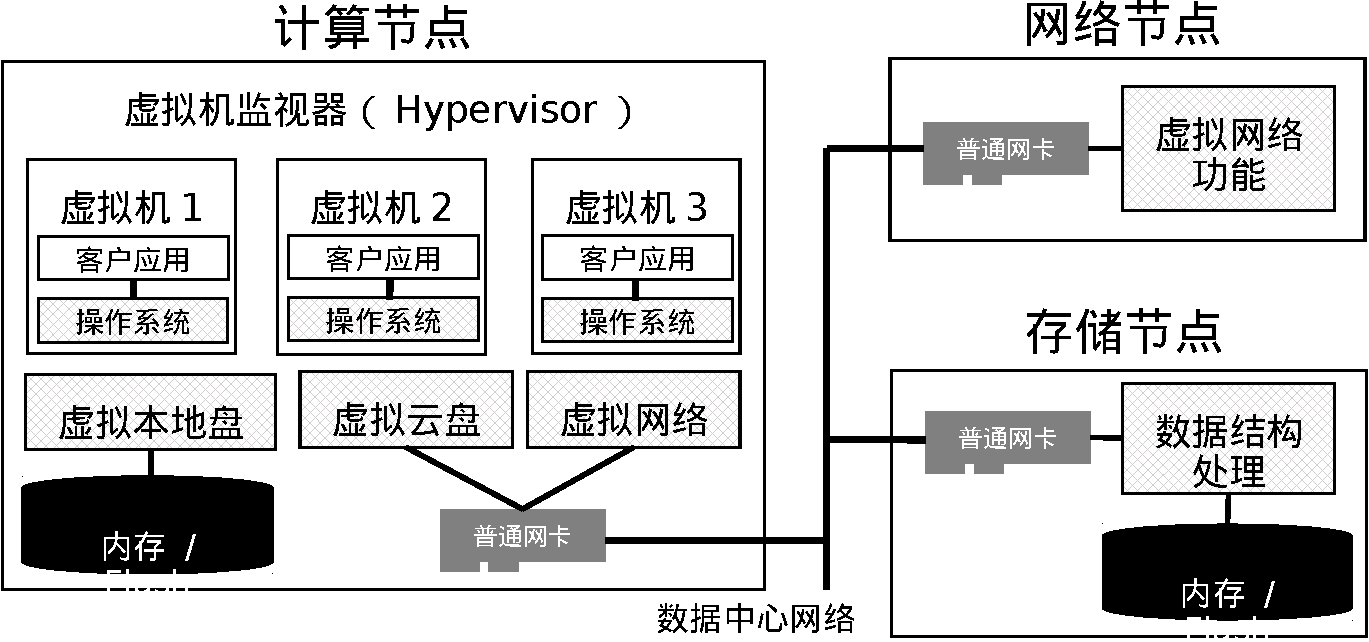
\includegraphics[width=0.8\textwidth]{figures/virt_arch.pdf}
	\caption{Virtualized data center architecture. The boxes with shaded backgrounds represent the costs of the data center, excluding the execution of customer applications, i.e., the "data center tax".}
	\label{background:fig:virt-architecture}
\end{figure}

\subsection{Virtual Networks}

In public clouds, major customers require more than just virtual machines; they also need the simulation of enterprise network architectures. To support network security features such as security groups and access control lists, as well as to conceal internal network structures on the internet and reduce attack surfaces, public cloud services provide Virtual Private Cloud (VPC) services. This involves partitioning a logically isolated section in the public cloud, offering rich network semantics, such as private virtual networks with customer-provided address spaces, security groups and access control lists (ACLs), virtual routing tables, bandwidth metering, Quality of Service (QoS), etc. Consequently, the network in the public cloud is virtualized, decoupling the virtual network from the physical network. As shown in Figure \ref{background:fig:network-architecture}, when two customer virtual machines on two computing nodes communicate, they need to go through the encapsulation and decapsulation of the virtual network software, and may also need to go through the processing of several network functions on the network node. Network functions will be the main topic of the next section.

\begin{figure}[htbp]
	\centering
	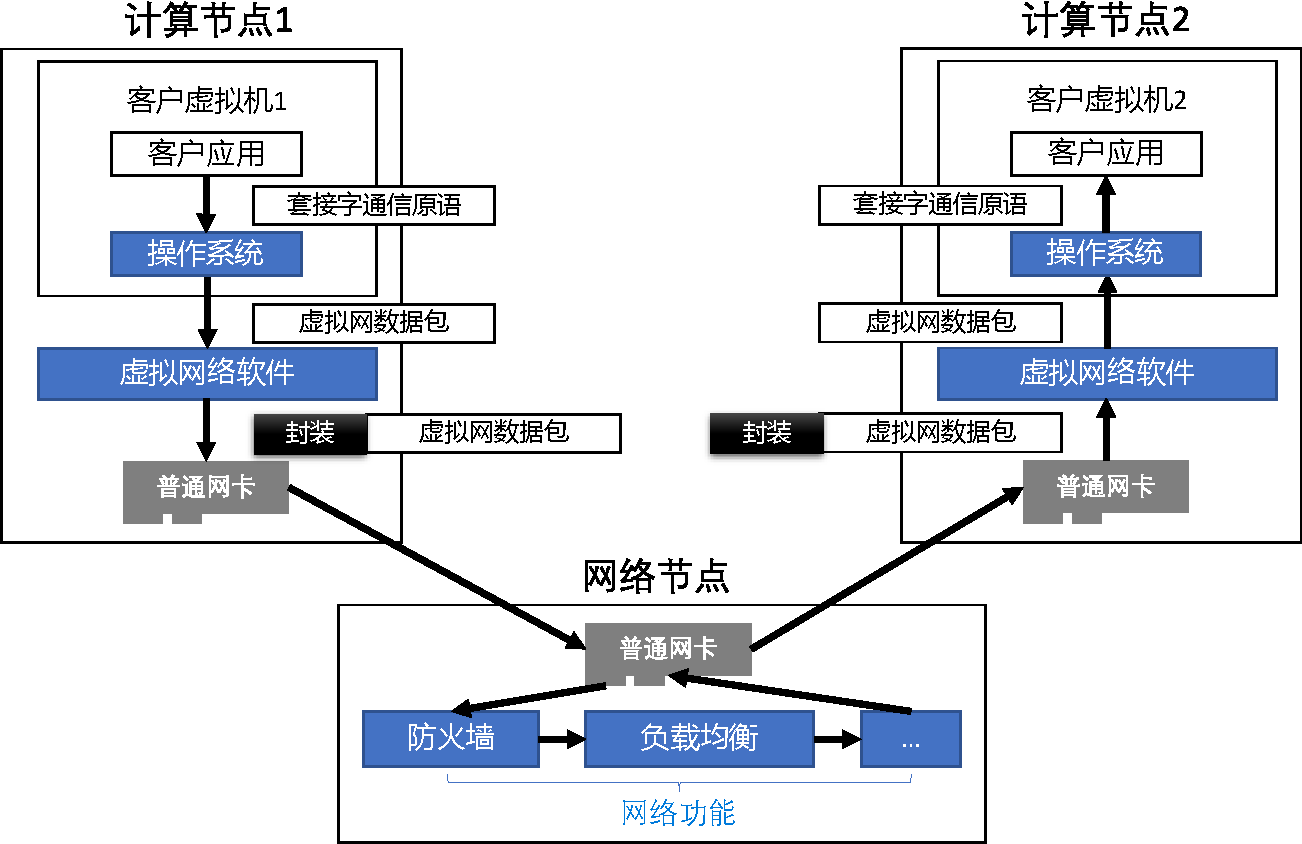
\includegraphics[width=0.8\textwidth]{figures/VPC_arch.pdf}
	\caption{Data center virtual network architecture.}
	\label{background:fig:network-architecture}
\end{figure}

The data plane of the virtual network can be described by a Match-Action Table, which can theoretically be implemented on commercial network switches. In 2007, Stanford University proposed OpenFlow \cite{mckeown2008openflow}, which unified the control plane interfaces of different vendor switches, allowing the network to be programmed by software, i.e., Software Defined Networking (SDN). To support the control plane of SDN, Onix \cite{koponen2010onix} proposed a control framework for large-scale switches, and programming languages like Frenetic \cite{voellmy2010nettle,foster2011frenetic} proposed using the Functional Reactive Programming (FRP) paradigm to simplify control plane event handling. Covisor \cite{jin2015covisor} implemented the virtualization of the control plane. As the programmability of switches increases, it becomes possible to define the data plane forwarding behavior of switches from top to bottom using software, rather than adapting to the fixed functions of switches from bottom to top like OpenFlow.

For this purpose, in 2013, Stanford University proposed P4 \cite{bosshart2014p4}, providing programmable packet parsing, stateful match-action pipelines, and other programming abstractions. The academic community has proposed various implementations of the P4 language on programmable switch chips \cite{bosshart2013forwarding}, programmable network cards \cite{kaufmann2016high}, FPGAs \cite{wang2017p4fpga}, and CPU virtual switches \cite{shahbaz2016pisces}. Industrial solutions like the Barefoot Tofino switch chip \cite{barefoot-tofino}, Mellanox Connect-X network card \cite{mellanox}, and the Xilinx SDNet network processor based on FPGA \cite{xilinx-p4} also support the P4 language.

However, virtual networks based on network switches face two fundamental challenges in cloud data centers. First, the semantics of actual cloud data center virtual networks are very complex and change too frequently, making it difficult for the update speed of traditional switch hardware with fixed functions to match the speed of demand changes. Second, a top-of-rack switch connects dozens of rack servers, each of which can virtualize dozens of virtual machines, so the switch needs to support the data plane encapsulation and forwarding rules of up to thousands of virtual machines. The lookup table capacity of existing commercial switch chips is insufficient. For this reason, Microsoft proposed a programming abstraction similar to P4, VFP \cite{firestone2017vfp}, to support host-based software-defined networking, implementing virtual networks in virtual switch software. Host-based virtual networks can scale well with the number of computing node servers and maintain the simplicity of the physical network.

In this network virtualization model based on virtual switches, every packet sent and received by a virtual machine is processed by the virtual switch (vSwitch) in the virtual machine monitor. Receiving packets usually involves the virtual switch software copying each packet to a buffer visible to the virtual machine, simulating a soft interrupt for the virtual machine, and then letting the network protocol stack of the virtual machine's operating system continue network processing. Sending packets is similar, but in reverse order. Compared to non-virtualized environments, this additional host processing reduces performance, requires additional changes to privilege levels, reduces throughput, increases average latency and latency variation, and increases host CPU utilization.

As shown in Figure \ref{background:fig:network-perf-trend}, the improvement speed of data center network performance far exceeds that of general-purpose processors. In a 10 Gbps network, only one CPU core is needed, while in the current 40 Gbps network, about 5 CPU cores are needed, and in the future 100 Gbps network, even 12 CPU cores may be needed. This brings about the "data center tax".

\subsection{Network Functions}
\label{background:sec:network-function}

In addition to virtual networks, data centers also require a variety of network functions. For example, large-scale Internet services have multiple front-end servers processing user requests concurrently, which requires a highly available, high-performance load balancer to accept user requests and distribute them to the front-end servers. Enterprise-grade load balancers may also support a series of advanced features, such as flexible load balancing rules based on user requests, HTTPS secure connections, log recording and statistics, detection and filtering of possible denial of service (DoS) attacks, Web application injection attacks, etc. \cite{ananta}.

Furthermore, many governments and enterprises already have their own IT information systems. If all are migrated to the public cloud, it does not meet some institutions' requirements for data privacy and security, and the cost and risk of one-time migration are too high. Therefore, it is necessary to connect the customer's existing IT information systems (on-premises) and virtual networks on the public cloud. In addition, in response to customer concerns about data security and privacy, many cloud vendors offer a private cloud (or dedicated cloud) mode, which deploys the software and hardware architecture of the public cloud on the customer's dedicated data center infrastructure. To support the connection between on-premises, private clouds, and public clouds, cloud vendors need to provide virtual private line services, which require a dedicated line gateway capable of implementing basic network functions such as encryption, routing, access control lists, as well as advanced network functions such as caching, TCP acceleration. In some cases, the connections between these clouds and between the cloud and the office are not through SDH or MPLS dedicated lines, but through the Internet public network. At this time, protocols such as IPSec are needed to encrypt and sign the data, using an IPSec gateway \cite{son2017protego}.

In addition, operator networks' data centers also run a large number of network functions. For instance, AT\&T operates over 5,000 Central Offices in the United States, each supporting tens of thousands of users, running Broadband Network Gateways (BNG) and Evolved Packet Core (EPC) gateways in the LTE network \cite{chang-lan-thesis}. Operators not only aim to reduce the assets and operating costs of the central office but also aspire to lease the edge computing resources of the central office to third parties \cite{chang-lan-thesis}.

Traditionally, these network functions are implemented using dedicated devices, such as F5's load balancer \cite{f5-load-balancer}, Distributed Denial of Service (DDoS) protection, Web Application Firewall (WAF), etc.; core router or F5 BIG-IP gateway provided by Cisco offers IPSec gateway functions; operators utilize core network equipment from companies like Huawei, Ericsson, etc. However, these dedicated hardware devices are costly and lack flexibility. Public clouds and 5G networks require flexible network functions to support secure and performance isolation between customers, to meet the Quality of Service (QoS) of different customers. Data center networks and 5G core networks need to support a variety of different service requirements on the same physical network. Such as the three typical application scenarios of 5G: extremely high bandwidth (eMBB), massive scale (MTC), extremely low and stable latency (URLLC). High bandwidth, large scale, low latency requirements are somewhat contradictory to some extent and need to be balanced according to the application's requirements. For high flexibility, data centers such as Amazon, Microsoft, Google, etc., have adopted virtualized software network functions to replace dedicated devices. The 3GPP standard also specifies that the 5G core network adopts a service-based system architecture, and these services need to be implemented using virtualized network functions \cite{3gpp-23501,3gpp-38300}.

Through the examples of load balancers, dedicated / IPsec gateways, and operator networks, it can be seen that the complexity of network functions is significantly higher than that of virtual networks. Virtual networks operate at the network layer, data link layer, generally only need to process packet header information, and do not need to maintain complex variable states; while network functions cover the application layer, transport layer, network layer, etc., need to process the payload of data packets, and need to find the network connection to which the data packet belongs based on the data packet, make processing based on the current state of the connection, and then update the state of the connection. The programming flexibility of P4 \cite{bosshart2013forwarding} is not enough to implement flexible payload processing and stateful processing based on connections.

In 2000, Professor Eddie Kohler of the Massachusetts Institute of Technology proposed Click \cite{kohler2000click}, a modular router programming framework. Click decomposes network processing into several basic elements (element), each element is implemented with a C++ class; the router's packet processing is a data flow graph composed of these elements, and the Click programming language allows flexible interconnection between these elements. Since the Click open-source project already has a large number of elements, many network researchers only need to interconnect these elements to assemble a complex network function; since Click uses C++ language programming, its flexibility is very high. Therefore, a series of recent research works \cite{martins2014clickos,netbricks} implement network functions based on the Click programming framework. E2 \cite{palkar2015e2} proposed a highly available, highly scalable network function scheduling and management framework. Chapter \ref{chapter:clicknp} of this paper will propose a high-performance network function processing platform that implements the Click programming framework on FPGA.

\subsection{Operating System}

The operating system mainly includes three aspects of functionality: resource virtualization, inter-process communication, and high-level abstraction. Resource virtualization refers to the sharing of computing, network, and storage resources among multiple processes in the operating system, which requires ensuring security isolation and performance isolation between processes. Inter-process communication includes message passing, shared memory, and synchronization primitives such as locks and semaphores. High-level abstraction is the abstraction of hardware resources into a unified interface that is easy to use for applications, such as the "everything is a file" model in Linux. The network is abstracted into sequential read-write socket connections, and storage is abstracted into file systems. This paper focuses on the network functions of the operating system, namely the sharing of network resources among multiple processes, inter-process communication based on message passing, and socket abstraction.

Distributed applications commonly use the socket primitives in the operating system for communication. As shown in Figure \ref{background:fig:kernel_time}, for communication-intensive applications such as HTTP load balancers, DNS servers, Memcached \cite{memcached}, and Redis \cite{redis} key-value storage servers, the operating system occupies 50\% to 90\% of CPU time, most of which is used to handle socket operations.

\begin{figure}[htbp]
	\centering
	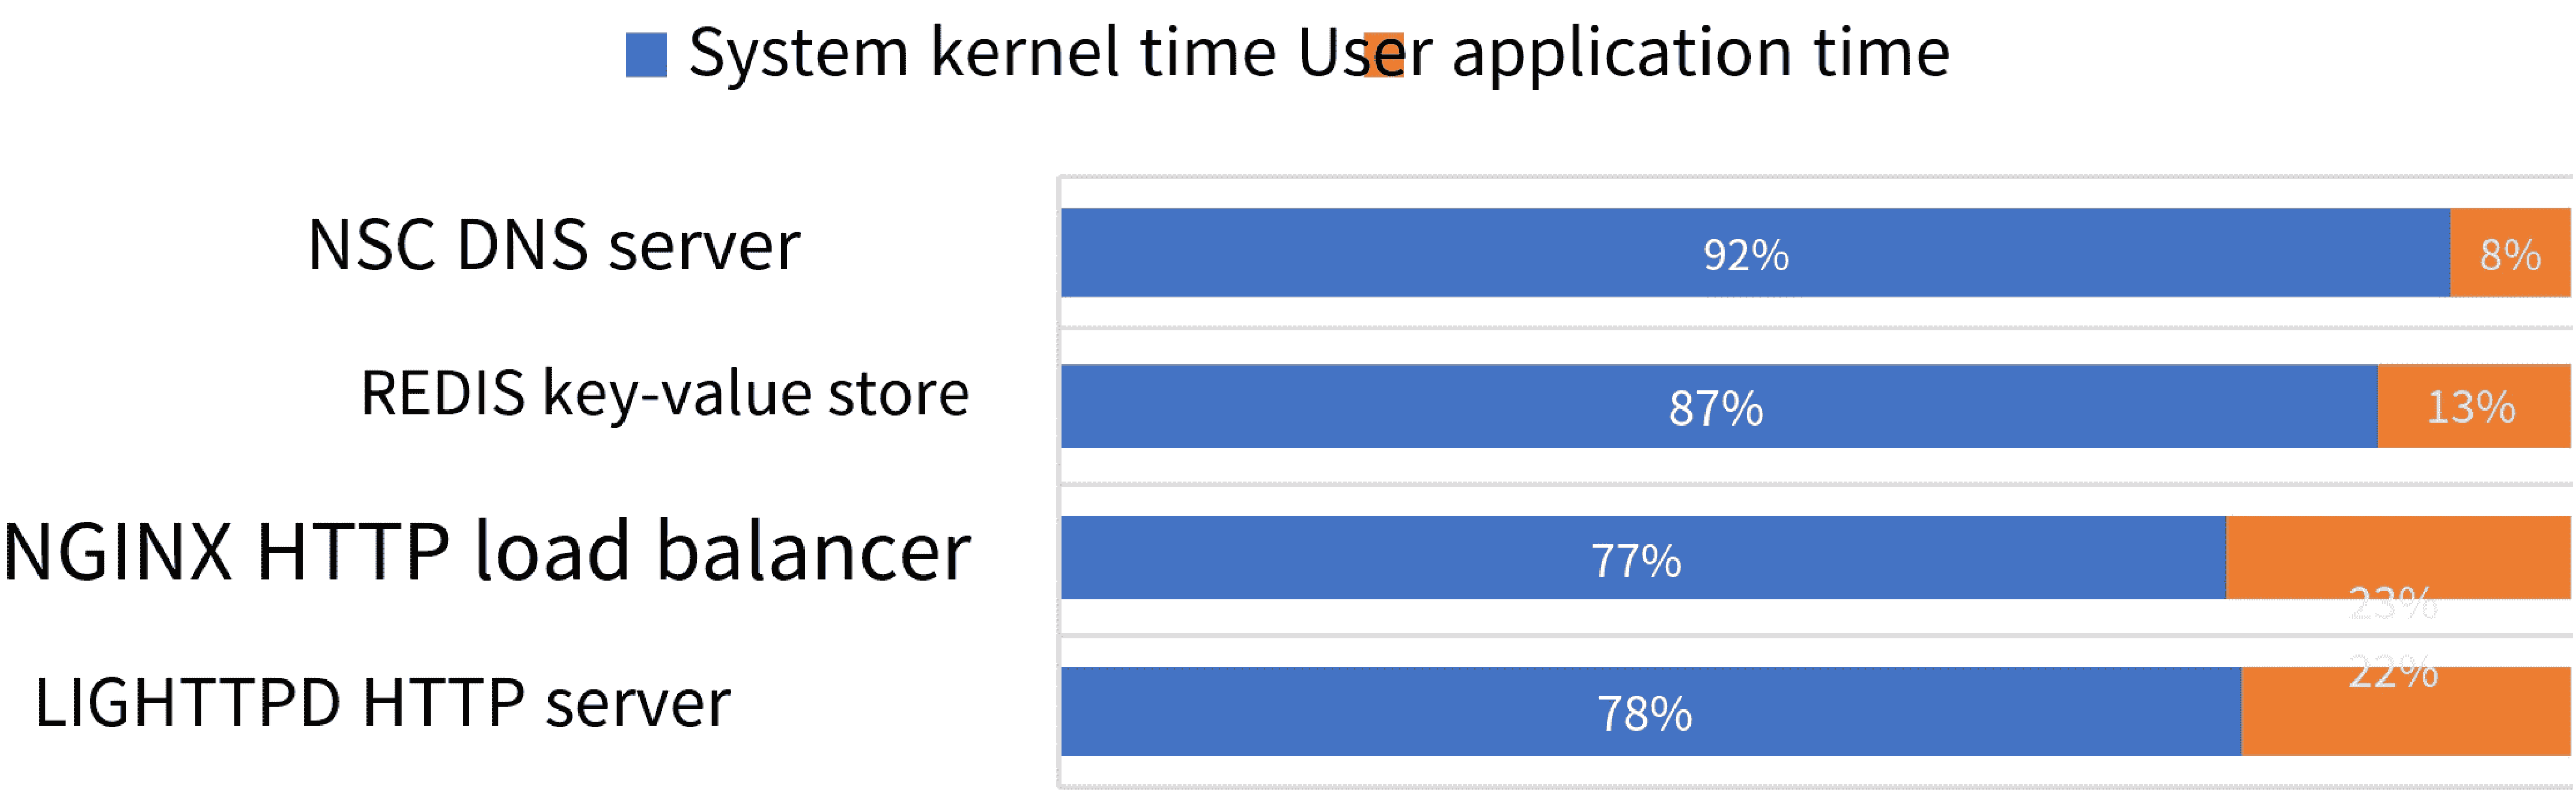
\includegraphics[width=0.8\textwidth]{figures/kernel_time.pdf}
	\caption{Communication-intensive applications consume a lot of CPU time in the operating system kernel.}
	\label{background:fig:kernel_time}
\end{figure}

In the Linux operating system, applications perform I/O operations through File Descriptors (FD). Conceptually, the Linux network protocol stack consists of four layers. First, the Virtual File System (VFS) layer provides a socket API based on file descriptors for applications. Second, at the transport layer, the traditional TCP transport protocol provides I/O multiplexing, congestion control, packet loss recovery, and other functions. Third, at the network and link layer, the IP protocol provides routing functions, Ethernet provides flow control and physical channel multiplexing at the data link layer, and Linux also implements Quality of Service (QoS) and firewalls based on the netfilter framework. Fourth, at the device driver layer, the network card driver communicates with the network card hardware (or the virtual loopback interface for sockets within the host) to send and receive packets.

It is well known that the virtual file system layer contributes a large part of the overhead of network I/O operations \cite {clark1989analysis,boyd2010analysis}. In Chapter \ref{chapter:socksdirect} of this paper, a simple experiment will verify that the latency and throughput of Linux TCP sockets between two processes in the host are only slightly worse than Linux pipes, FIFOs, and Unix domain sockets. Pipes, FIFOs, and Unix domain sockets bypass the transport layer and network card layer, but their performance is still not satisfactory.

Using the Linux network protocol stack as an example, its overhead is multifaceted. For each I/O operation, a kernel crossing is necessary, and a file descriptor lock must be obtained to safeguard multi-threaded concurrent operations. Each packet's sending and receiving involve a series of operating system overheads such as transport protocol, buffer management, I/O multiplexing, interrupt handling, and process awakening. Each byte's sending and receiving require multiple memory copies. Each establishment of a TCP network connection necessitates the allocation of kernel file descriptors and TCP control blocks, and the TCP server side also needs to schedule new connections. These overheads will be discussed in detail in Chapter \ref{chapter:socksdirect}.

Chapter \ref{chapter:socksdirect} of this paper will propose a user-space network protocol stack, which transfers the overhead of the operating system's network protocol stack to the user-space library and programmable network card, achieving network transmission close to hardware performance.

\subsection{Data Structure Processing}

Traditional software-based memory data structure storage systems need to access the network through the operating system kernel at both the client (computing node) and server side (storage node), and also need to handle concurrent access to shared data structures through software, bringing a series of overheads.

The overhead of the operating system kernel has been discussed in the previous section. Even if these overheads are completely eliminated, the throughput bottleneck of memory data structure processing is still limited by the computation in data structure operations and the latency in random memory access. On the one hand, CPU-based key-value storage needs to spend hundreds of CPU cycles to perform key comparisons and hash slot calculations. On the other hand, the hash table of key-value storage is several orders of magnitude larger than the CPU cache, so the waiting time for memory access is determined by the cache miss waiting time of the actual access pattern. Chapter \ref{chapter:kvdirect} will analyze in detail that even if all CPU cores process key-value operations, their throughput is still far lower than the random access capability provided by the host DRAM memory. For this reason, Chapter \ref{chapter:kvdirect} will propose a memory data structure storage based on programmable network cards.

Why is the energy issue so critical to the future of the information industry?
In 1961, Qian Xuesen predicted, "People have long harbored the desire to fly in space... Interstellar travel will be the most remarkable achievement of science and technology in the second half of the 20th century." \cite{qianxuesen}
Regrettably, contrary to the forecasts of eminent scientists like Qian and science fiction authors like Arthur C. Clarke, the exploration of interstellar travel, despite fostering the significant advancement of numerous sciences and engineering technologies, has not become a widespread technology due to energy and material constraints.
Nevertheless, Information and Communication Technology (ICT) has emerged as the most brilliant new star in science and technology since the end of the 20th century, thanks to the exponential performance improvement predicted by Moore's Law.

Since information is intangible, the performance of integrated circuits per unit area can be enhanced by making the storage and processing units increasingly smaller, thereby augmenting the number of storage and processing units per unit area. This is the original statement of Moore's Law.
More profound is Dennard's scaling law \cite{dennard1974design}, which posits that the performance of integrated circuits can double every two years without consuming more energy and area.
Its theoretical foundation is that a new semiconductor process is adopted every two years, the transistor size is reduced by 30\%, and the chip area is reduced by 50\%. To maintain a constant electric field, the voltage is reduced by 30\% in proportion to the transistor size. Simultaneously, because the chip size is reduced, the delay is reduced by 30\%, and the clock frequency can be increased by 40\% \cite{borkar1999design,borkar2011future}.
In that era, the dynamic power consumption of integrated circuits accounted for the main part of power consumption, which is directly proportional to capacitance, the square of voltage, and frequency, so it can be calculated that power consumption is reduced by 50\%.
According to this ideal model, the area and power consumption of integrated circuits are halved every two years, so twice the number of transistors can be packed into the original area and power consumption, and the clock frequency is also increased to 1.4 times.
For single-threaded microprocessors with von Neumann architecture, these additional transistors are primarily used for larger caches, more complex pipelines, superscalar, out-of-order execution, register renaming, branch prediction, etc., to increase the number of instructions that can be executed per clock cycle.
According to Pollard's empirical law \cite{pollackpollack}, the computing power per clock cycle is roughly proportional to the square root of the number of transistors.
The computing power per unit time is equal to the clock frequency multiplied by the computing power per clock cycle, so the performance of the microprocessor is doubled every two years without consuming more energy and area.

The rate of performance enhancement in information systems is unparalleled in other industries dealing with macro tangible objects. In 1976, the Concorde broke the sound barrier, but it was not economical due to high fuel consumption. Modern passenger planes, like most passenger planes 50 years ago, still fly at subsonic speeds. And the massive system innovation from ordinary speed trains to high-speed trains has only increased the operating speed by more than 2 times. Currently, the primary source of energy for humans is fossil energy. Due to its usage cost and environmental impact, energy remains a significant constraint on the development of all industries before major breakthroughs in new energy technologies \cite{energy}. Compared with data centers, mobile terminals, and Internet of Things devices are more sensitive to power consumption because the energy density of batteries is increasing slowly, and these devices are very sensitive to volume and weight.

Regrettably, since the 21st century, the dividends of Moore's Law and Dennard's scaling law are gradually disappearing. First, as the feature size of integrated circuits decreases, the voltage also decreases. But the lower the threshold voltage that controls the transistor, the faster the leakage current of the transistor will increase, becoming a significant part of the power consumption of integrated circuits. To control the leakage current, the threshold voltage cannot be reduced, and even needs to be higher than the previous generation of integrated circuits \cite{borkar1999design}. Therefore, for each new generation of semiconductor processes, the power consumption per transistor will not be halved as expected. Secondly, because the area of each transistor is halved and the power consumption is not reduced so much, the power consumption of integrated circuits per unit area will increase. Currently, the power consumption of a 100 square millimeter chip is about 65 watts \cite{borkar2011future}, making it one of the highest power density controllable devices in humans, and the power density per unit volume is even comparable to that of aero engines. Therefore, the heat dissipation problem of the chip has become a major factor restricting the scale of integrated circuits. Third, for the same integrated circuit, in order to double the performance and double the clock frequency within the allowable range, the voltage must be doubled to reduce the flip delay of the transistor, so the power consumption is roughly proportional to the cube of the clock frequency. Due to the limitation of heat dissipation, the clock frequency of integrated circuits is also limited, and it is unrealistic to significantly improve the performance of integrated circuits by "overclocking". Finally, the 7 nm semiconductor process has been mass-produced, and the radius of a silicon atom is 0.1 nm. As the feature size of integrated circuits gets closer and closer to the atomic size, quantum effects cannot be ignored, which brings great technical challenges to lithography technology \cite{borkar2011future}. In fact, since around 2010, the reduction in the feature size of integrated circuits has significantly slowed down and can no longer maintain the speed of one generation every two years. In summary, under the current semiconductor technology framework, the performance of integrated circuits per unit area can no longer maintain a doubling speed every two years, and performance improvement also means power consumption increase, the "free lunch" is over.

In the realm of communication technology, channel coding has progressed from the relatively inefficient Hamming codes and Golay codes to convolutional codes, and then to Turbo codes that approach the Shannon limit, LDPC codes unearthed from stacks of old papers, and Polar codes that theoretically reach the Shannon limit. Given a constant physical channel and signal-to-noise ratio, the throughput of the communication system gradually approaches the Shannon limit.
In fact, Turbo codes are extensively used in wireless communication standards such as HSPA, LTE, WiMAX, etc., LDPC codes are used in 5G eMBB data channels, IEEE 802.11n wireless local area networks, WiMAX, etc., and Polar codes are also used in 5G eMBB control channels, etc.
The performance enhancement of modern wireless communication systems no longer primarily relies on the improvement of channel coding, but mainly depends on higher bandwidth physical channels, MIMO, improved multiple access technology, improved channel estimation and interference management, relay and other air interface technologies, as well as the cloudification and microservice of the core network \cite{3gpp-23501,3gpp-38300}. Many of these aspects depend on the improvement of computing performance, for example, the delay and throughput requirements of 5G core network data plane processing have significantly increased, and technologies such as MIMO have also added a lot of computing, so they are still subject to the performance of integrated circuits.
If the performance of computing, storage, and communication systems only grows linearly by consuming more energy and materials, it is clearly neither economical nor sustainable.

\subsection{The Scope for Full-Stack Optimization in Data Centers}

In an era where the dividends of Moore's Law and Dennard Scaling are gradually diminishing, can we continue to enhance the performance of computation, storage, and networking to maintain the rapid development of the information industry? The answer is affirmative. In the long run, new technologies such as quantum computing, DNA storage \cite{bornholt2016dna}, optical storage \cite{glass-a-new-media-for-a-new-era}, and optical switching \cite{farrington2011helios} have infinite possibilities. In the short term, there is still a lot of room for optimization in the performance of current computer systems based on semiconductor integrated circuits. There is still an opportunity to "squeeze so much juice out of this lemon of Moore's Law" \cite{threebody}, which is also the focus of this article. The following will discuss from the perspectives of chip architecture, operating system, software, and data center respectively.

Firstly, from the perspective of chip architecture, the traditional von Neumann architecture cannot fully utilize the computing power of each transistor. Theoretically, the computing power per clock cycle can be proportional to the number of transistors, but the aforementioned Pollard's empirical law \cite{pollackpollack} points out that the computing power per clock cycle is actually proportional to the square root of the number of transistors. For example, the world's first microprocessor Intel 4004 in 1971 used a 10-micron process, had 2300 transistors, a clock frequency of 108 KHz, and could perform 90 K 4-bit operations per second. The Intel Xeon E5 microprocessor based on the Broadwell architecture in 2016 used a 14-nanometer process (1M times of 4004), had 7.2 billion transistors (3M times of 4004), a base frequency of 2.2 GHz (20K times of 4004), and could perform about 300 G 64-bit operations per second \footnote{Assuming the application uses AVX2 instructions, does not use FMA3 instructions, and does not overclock.} (3M times of 4004) \cite{intel-e5-v4}. It can be seen that the number of operations that Xeon E5 can perform per clock cycle is about 150 times that of 4004, while the number of transistors is 3 million times. Even considering the complexity of 64-bit computing compared to 4-bit computing, it still means that the contribution of each transistor in 4004 to computing power is hundreds of times higher than that of Xeon E5. This is because the instruction set and microarchitecture of von Neumann architecture microprocessors are becoming more and more complex, one is to improve single-thread performance, the second is to add deeper cache levels to solve the "memory wall" problem, and the third is to support communication and synchronization between cores, operating systems, and virtualization technologies. The proportion of transistors actually used for computation is getting smaller and smaller.

Due to the performance bottleneck of von Neumann architecture processors, customized hardware has become a trend. The basic operations of customized hardware do not need to be expressed through instructions, and the data operation process is relatively fixed, so there is no need for the overhead related to instruction decoding execution and pipeline control of von Neumann architecture. Customized hardware can customize data paths and memory levels, avoiding the "memory wall" problem of shared access to all memory addresses in von Neumann architecture. Customized hardware can build a large number of processing units to parallel process the same type of data (such as matrix operations), or a deep pipeline to process deep logic level calculations (such as symmetric encryption). As shown in Figure \ref{background:fig:moores_law_redefined}, the energy efficiency of Nvidia GPUs such as K80, P100, P40, V100, Intel FPGAs such as Arria 10, Stratix 10, and Google's deep learning processor TPU is much higher than that of general-purpose processors (note that the y-axis is a logarithmic coordinate system), and basically follows Moore's Law in terms of performance, that is, the energy efficiency of customized hardware doubles every 18 months.

\begin{figure}[htbp]
	\centering
	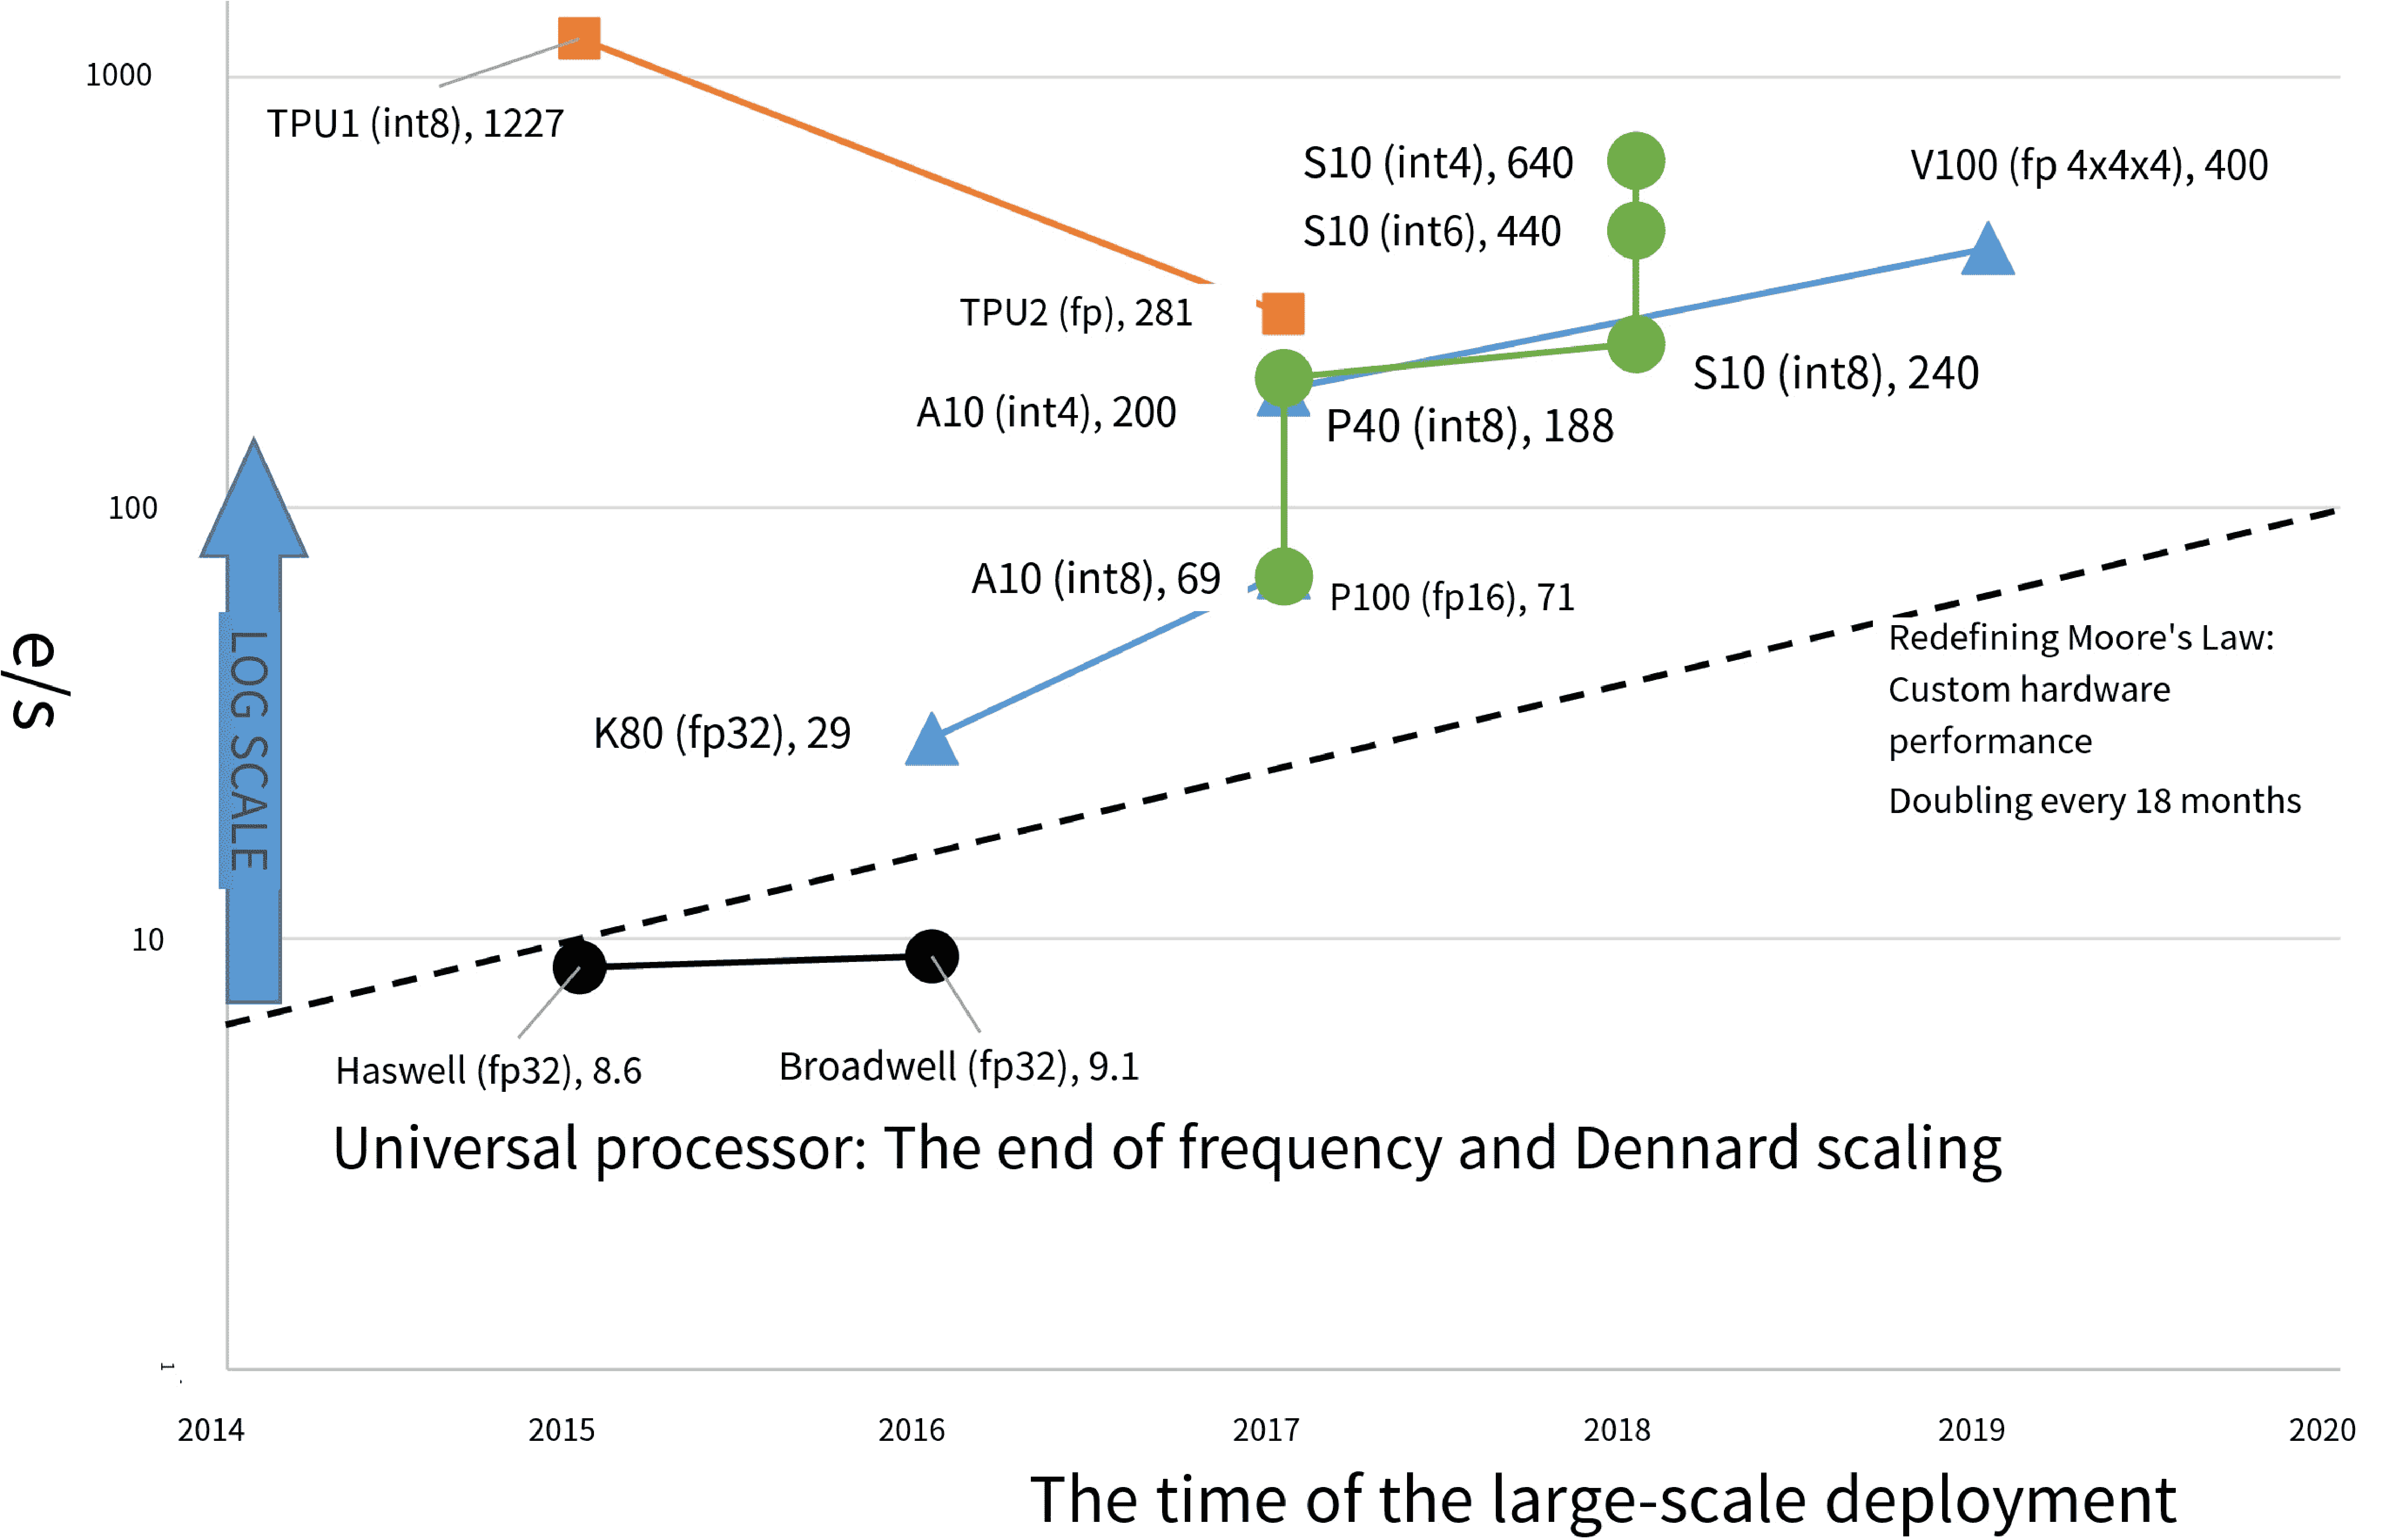
\includegraphics[width=0.8\textwidth]{figures/moores_law_redefined.pdf}
	\caption{The frequency of general-purpose processors and Dennard scaling gradually end, but customized hardware redefines and continues Moore's Law.}
	\label{background:fig:moores_law_redefined}
\end{figure}

The rapid enhancement in the performance of customized hardware primarily stems from two aspects. On one hand, due to the high one-time research and development cost (NRE) of more advanced processes, in the initial phase of a field transitioning from general computing to customized computing, customized hardware employs a more outdated, lower-cost process. As the computing power demand in this field escalates and chip design experience accumulates, more advanced processes are gradually adopted. General-purpose processors have been utilizing almost the most advanced processes due to years of accumulation and massive production volume. On the other hand, the design of customized hardware is also continuously optimized, and it is also optimized in conjunction with applications. For instance, in deep learning, many models can reduce the computational load and maintain prediction accuracy by reducing parameter accuracy and sparse expression. In Figure \ref{background:fig:moores_law_redefined}, the energy efficiency of the same Arria 10 FPGA chip performing 4-bit integer operations is about 4 times that of 8 bits.

Secondly, the optimization space of the operating system is also substantial. The previous section has indicated that the large overhead of network and storage protocol stacks as a significant part of the "data center tax" is worth optimizing.

Thirdly, modern software reaps the benefits of Moore's Law. For the sake of development efficiency, it generally employs high-level language modular programming, and the compiler's optimization of software is not sufficient. Modern software written in high-level languages, even if its functions are similar to those of software based on low-level languages (such as C language) many years ago, its performance often differs significantly. The "Andy-Bill's Law" \cite{langchaozhidian} vividly illustrates this phenomenon, that is, the performance added by high-performance new processors (represented by Intel's CEO Andy) is often consumed by software (represented by Microsoft's founder Bill Gates), and the performance perceived by end users remains similar. There is also a considerable room for optimizing software performance from the perspectives of programming frameworks, compilers, etc. David Patterson pointed out that rewriting Python language into C language can enhance the performance of the application by 50 times, and if a series of optimizations are used, achieving a performance improvement of 1000 times compared to Python is not a dream \cite{python-to-c}. The hardware-software combined acceleration in this article can be considered as an attempt in this regard. After dividing the software according to the data plane and control plane, the performance-sensitive data plane uses hardware acceleration, while the control plane still uses software to provide development efficiency and flexibility.

Fourthly, the resource utilization rate of contemporary data centers is low, presenting a significant opportunity for optimization. For instance, the average usage rate of most physical servers in data centers is only about 10\% to 15\%, yet the power consumption during idle periods is only 30\% less than at peak usage \cite{barroso2018datacenter}. On one hand, the energy-saving design of servers and hardware can be enhanced to minimize power consumption as much as possible when the usage rate is low or even idle. On the other hand, one of the benefits of cloud computing is that it supports live migration. In theory, it can package virtual machines with complementary demands on a physical server host according to the computing, memory, storage, and network requirements of the virtual machine, maximizing the utilization of various hardware resources of the physical server. Currently, due to various technical constraints, live migration causes a period of performance degradation or even interruption to customer services, so its use in cloud computing is not widespread.

In cloud computing platforms, both software and hardware environments are controlled by service providers. Once a certain scale is reached, all forms of customization become possible. As long as it can enhance performance, reduce costs, and improve competitiveness, cloud service providers have sufficient motivation to customize chips, alter network protocols, change server architectures, modify operating systems, and even rewrite applications.

In conclusion, the demand for data center applications, the performance limitations of general-purpose processors, and the trend of cloud computing scale make full-stack optimization of software and hardware a trend in data centers. System performance optimization can not only save costs and meet customer performance requirements, but also simplify system architecture and reduce trade-offs in design. For example, if the overhead of virtualization is reduced under a fixed application layer latency budget, more complex calculations can be performed to achieve more accurate and real-time results; if the latency of remote procedure calls is reduced to 1/3, an application layer request can call 3 times the number of remote procedure calls, facilitating the decoupling of backend microservices. If the performance of key-value storage is high enough, there is no need to add extra cache at the application layer, reducing the reinvention of the wheel and avoiding potential problems of cache inconsistency. If the performance of socket communication primitives is high enough, applications do not need to be modified to use more complex communication primitives such as RDMA.

If the performance optimization of the above existing systems is a negative motivation, system performance optimization also has a positive motivation, that is, to propose efficient abstractions and empower more applications. For example, high-bandwidth, low-latency RDMA networks make large-scale deep learning and data processing possible. In traditional low-speed networks, the overhead of communication may be higher than the benefits of distribution. Solid-state storage (SSD) has changed the design paradigm of storage and database systems, making random access and real-time processing of big data possible; non-volatile storage (NVM) will bring greater changes. Looking at a larger category outside the data center, GPUs were initially used for display cards and graphics computing acceleration, but in recent years they have become the main computational support for deep learning; 4G mobile networks, with their larger bandwidth and lower unit traffic cost compared to early mobile networks, have boosted the rapid development of the mobile Internet. The highest mission of data center infrastructure researchers is to propose universal abstractions, so that developers can reliably and efficiently implement applications based on these abstractions. The desire to propose such abstractions is the source of endless perseverance and patience in data center performance optimization work.

This article is dedicated to using full-stack optimization methods to reduce the "data center tax" and improve the performance of fine-grained computing represented by virtualization and large-scale distributed systems. The next section will introduce the development trend of data center hardware and introduce the new data center hardware introduced in this article: programmable network cards.

\iffalse

\subsection{The Development of Chips}

The progress of computer architecture is inseparable from the development of semiconductor integrated circuits. It can be said without exaggeration that the development of computers is the biggest driving force for integrated circuit technology, as well as the biggest beneficiary. Over the past half century, integrated circuits have been developing at roughly the speed predicted by Moore's Law. Highly integrated chips have brought about one revolution after another in computer architecture, from mainframes to desktops, from servers to cloud computing platforms, from laptops to mobile computing. Integrated circuits have quickly permeated all aspects of life. On the other hand, it is the demand for computing that has driven the development of central processing units (CPUs), memory (DRAM), graphics accelerators (GPUs), and high-speed network chips. Chip technology and computer architecture complement each other, jointly promoting the development of computer system software and computer applications, making information technology so important in society and the economy in just a few decades.

Currently, information science and technology are still in a stage of rapid development, with new applications emerging one after another: artificial intelligence, the Internet of Things, virtual reality, blockchain, emerging directions are dazzling, each technology has infinite potential, and may push human society into a completely new future. On the other hand, CMOS integrated circuit chip technology based on semiconductor silicon is beginning to reach a bottleneck due to physical law limitations. On the one hand, it is challenging to further reduce the linewidth (Feature Size) of chips below 5 nanometers, and on the other hand, power consumption and heat dissipation have become difficult problems for modern chip technology to bypass. Under these circumstances, where will computer technology go? How will future computers meet the growing demand for computing power?

This brief article explores the possible directions of computer system development in the next few years, particularly how integrated circuit technology will continue to mutually promote with computer architecture, improve the speed and efficiency of computing, and meet the growing demand for computing power. The consensus in academia and industry is that scientists are unlikely to find a technology that can replace CMOS in the short term, so the improvement of computer technology performance in the short term must mainly rely on innovation in computer architecture. This brief article focuses on the possible development trends and directions of cloud computing platform architecture. In the foreseeable future, cloud computing will be a very important computing platform, it will provide the main computing power for human society, and promote the world's data processing capabilities. Of course, mobile computing, the Internet of Things, and other "ends" are also very important development directions, but due to space limitations, this brief article will not discuss these aspects of development in detail.

\subsection{Transformation of Cloud Computing Platforms}

At the dawn of the 21st century, as the concept of cloud computing was just beginning to take shape, the platform for cloud computing was essentially a typical corporate data center, albeit on a larger scale. The cloud computing of that era was markedly different from the supercomputing platforms used for scientific computing in terms of hardware. Supercomputers for scientific computing often utilized custom chips and networks, pursuing the highest performance regardless of cost. The hallmark of cloud platforms was to scale up ordinary low-end commercial servers, achieve high fault tolerance and reliability through software, reduce costs, and provide high-performance services.

As the business model of cloud computing gained user acceptance, particularly with the widespread acceptance of the public cloud concept, after nearly two decades of development, the primary cloud computing platform providers have achieved tremendous commercial success. The scale of cloud computing platforms has significantly expanded. The industry-leading cloud platforms now have hundreds of data centers scattered around the globe and millions of servers. This presents many new challenges to computer architecture. Constructing a large-scale cloud computing platform requires massive investments, and any innovation that can reduce the cost of a single machine can yield extremely high returns; cloud computing requires a lot of electricity to maintain operation, improving system efficiency and reducing power consumption are important indicators; a major selling point of the cloud computing platform is flexible and elastic configuration, how to provide elasticity while minimizing system idle is a complex problem; cloud computing needs to ensure reliability, needs to be easy to manage, needs to protect private information, there are many challenges here that need to be addressed.

In the early stages of computer development, hardware and software were developed by the same company team, and many groundbreaking technologies were invented and created in this environment, which had a profound impact on subsequent generations. With the evolution of computers, the design division of labor has become increasingly detailed, and the components of the computer such as CPU, memory, network, operating system, etc., are gradually completed independently by various professional companies, which forces engineers to comply with the existing system framework, and cross-disciplinary innovation has become very difficult. Although in some specialized fields (such as game consoles) designers may still consider the whole system, it has almost become an impossible task in the field of general computing.

\subsection{Field Programmable Gate Array (FPGA) and Application Specific Integrated Circuit (ASIC)}

To better comprehend integrated circuits and computer architecture, it is essential to briefly introduce two significant integrated circuit technologies.

ASIC (Application Specific Integrated Circuit) is an integrated circuit chip specifically designed for certain applications. The threshold for ASIC development is relatively high, and the research and development cycle is also comparatively long. With the current technological level, the one-time development cost (NRE, Non-Recurring Engineering) for a medium-complexity ASIC will be around several million to ten million dollars, and it will require a development cycle of one to two years.

FPGA (Field Programmable Gate Array) is a reconfigurable integrated circuit component. Intuitively, an FPGA is a large number of electronic components that can be recombined through programming. These components include logic gates (such as AND, OR, NOT gates), registers, adders, static memory (SRAM), etc., and users can customize their connections to form different circuits. Today's FPGAs, in addition to basic components, are also incorporating more and more DSPs and hard cores (hard IP) to improve multiplication, floating-point operation, and peripheral device access performance. The advantage of FPGA is that the technology is mature, the development threshold is relatively low compared to other integrated circuits (such as ASIC), and it can still be modified after deployment. The disadvantage is that the performance is inferior to that of dedicated chips.

Traditionally, FPGAs have been extensively used in prototype design, logic circuit simulation, and high-end routers, etc. In recent years, FPGAs have been increasingly used in data centers. In data centers, FPGAs are primarily used in two aspects, one is for applications that may still need to be changed after deployment, such as network cards. Since the network cards on the public cloud often need to adjust or add protocols, they need to frequently reprogram the hardware. Another application is computational acceleration: for some special computations, the highly parallelizable nature of FPGA can be used for acceleration. A rough rule for using FPGA to accelerate applications in data centers is the 10, 100, 1000 rule: the application needs to be accelerated by more than ten times, if the acceleration ratio is too small, it is not worth implementing in hardware; the accelerated part of the core is roughly equivalent to less than 100 lines of code, more complex logic is difficult to implement in hardware; and the computation in the data center should require at least around 1000 servers, if the number of servers is far less than 1000, it may not be worth developing a hardware solution. Of course, these numbers are very rough estimates and should be adjusted according to the deployment situation of FPGA, the value of the application itself, and the actual situation of the developers.

In the past, the development of Application-Specific Integrated Circuits (ASICs) was often a task that only professional hardware chip companies could undertake. However, with the continuous expansion of cloud computing platforms, companies operating these systems have also begun to attempt to design dedicated chips for their own clouds independently.

\fi

\iffalse
\section{Development Trends of Data Center Hardware}
\label{background:sec:hardware}

Modern computer systems can roughly be divided into four main parts: Compute, Memory, Storage, and Networking and Interconnect.

\subsection{Compute System}

The compute system is the core of the entire computer, typically composed of a Central Processing Unit (CPU) and some accelerators serving special applications. When considering the development of the entire computer architecture, innovation in the compute system may be the most closely watched area.

In the past, computing systems were essentially equivalent to CPUs, and innovations on CPUs were dominated by a few large companies such as Intel and IBM. Traditionally, computing power was a relatively abundant resource in computer systems. On one hand, thanks to Moore's Law and the advancement of CPU architecture, the speed and efficiency of CPUs have made significant progress; on the other hand, other subsystems such as hard drives, memory, and networks often become bottlenecks in practical applications due to their relatively slow progress. This situation has changed significantly in recent years: with the emergence of new hardware such as solid-state drives and high-speed networks, I/O is often no longer a bottleneck; and new applications such as deep learning and in-memory databases have a great demand for computing power, and traditional CPUs are increasingly difficult to support these applications. For this reason, innovation in computing systems, or what is commonly referred to as heterogeneous systems, has become a hot spot in computer architecture research in recent years.

\subsubsection{Deep Learning Accelerators}

The recent surge in interest in deep learning has made computing acceleration a hot topic. From universities to industry, from start-ups to industry giants, from traditional semiconductor companies to traditional application software developers, all are trying to design hardware accelerators specifically for deep learning applications, designing solutions for small low-power IoT devices to entire data centers. In the field of cloud computing, Google, as the pioneer of using integrated circuit ASICs to accelerate deep learning, has designed a dedicated Tensor Processing Unit (TPU) for this purpose, which has now developed to the third generation \cite{tpu}, and has achieved great success in terms of technological innovation, attracting attention, and commercial operation. Microsoft's use of Field-Programmable Gate Arrays (FPGAs) for Deep Neural Network (DNN) acceleration has also been launched on the Azure cloud platform \cite{serving-dnns-real-time-datacenter-scale-project-brainwave,a-configurable-cloud-scale-dnn-processor-for-real-time-ai}.

Deep learning encompasses both training and inference scenarios. Training requires substantial memory and complex operations, most of which are deployed in cloud data centers. NVIDIA's GPUs hold a significant ecosystem advantage, with only a few deep learning accelerators such as the third-generation TPU and Graphcore \cite{graphcore} posing a challenge to its monopoly. The application scenarios for inference are more heterogeneous. In mobile computing scenarios, low power consumption is the primary requirement, as exemplified by Cambricon's neural network processor integrated into Huawei's Kirin 970 mobile processor via intellectual property (IP) licensing. In search recommendation, autonomous driving, and virtual reality scenarios, both millisecond or even microsecond low latency and high throughput are required. Not only do various inference scenarios have different performance indicators, but they also require different neural network operations. In addition to supporting classic neural network operations such as recurrent neural networks, convolution, matrix multiplication, and regularization, accelerators also need to co-evolve with scenario-related algorithms. They must utilize sparsity \cite{yao2018balanced,cao2019efficient}, quantization \cite{zhang2015optimizing}, and other technologies to enhance computing power without reducing accuracy, and support emerging neural network structures such as dynamic control flow.

\subsubsection{FPGA and Reconfigurable Hardware}

The use of FPGAs for computing acceleration has been a topic of academic research for many years and has been applied in some specific fields. However, the large-scale deployment of FPGAs on general servers has only begun to make breakthroughs in recent years. Many companies have started to make some attempts in this area, especially Microsoft and Baidu have done a lot of work in effectively using FPGAs for cloud computing acceleration. For example, Microsoft has fully deployed FPGA modules on the Azure cloud platform \cite{putnam2014reconfigurable,caulfield2016cloud}. Baidu uses FPGAs for data compression \cite{ouyang2010fpga}, database SQL processing \cite{baidu-fpga-sql}, deep learning \cite{ouyang2014sda} and other rich application scenarios \cite{ouyang2017xpu}. At present, cloud vendors also provide FPGAs as a service to third-party developers. With the improvement of the FPGA development environment and development tools in the cloud, more and more applications will take advantage of the reconfigurability of FPGAs to achieve acceleration.

Following the acquisition of Altera, Intel introduced a Xeon chip integrated with FPGA, which connects the FPGA and CPU via the UPI (formerly QPI) bus, enabling coherent communication between the CPU and FPGA. This will significantly enhance the communication efficiency of the FPGA when used as a CPU accelerator. In contrast, Xilinx has launched a novel Versal reconfigurable hardware architecture \cite{vissers2018keynote,vissers2019versal,gaide2019xilinx}, which integrates reconfigurable hardware (FPGA), VLIW-based deep learning and traditional machine learning accelerators, digital signal processors (DSP) and hard IP, as well as multicore general processors on a single chip to form a System on Chip. 

The key distinction of the Versal architecture compared to traditional FPGAs is that it forms a system on a chip, which is evident in three aspects: firstly, it hardens the control logic of external interfaces such as memory controllers and PCIe into digital logic from the reconfigurable logic, reducing the area overhead of FPGAs and enabling FPGAs to achieve plug and play. Secondly, it acknowledges the low efficiency of implementing common computations such as vector operations in big data and machine learning on FPGAs, and accelerates them with hardened digital logic. Thirdly, it incorporates a general processor that can handle complex logic and control planes without having to loop back to the CPU, allowing the Versal system on a chip to directly drive Flash storage and other components, forming a low-cost storage server without the need for traditional x86 CPU components. The components of the system on a chip are interconnected through an on-chip network \cite{swarbrick2019network,gaide2019xilinx}. 

The Versal architecture is designed to accelerate a variety of applications in data center servers. Developers can decompose applications into control planes on general processors, data planes on reconfigurable hardware, and data planes on vector computations, using the appropriate architecture to handle the corresponding parts of the application. These technologies will have a profound impact on the architecture of cloud computing platforms in the coming years. 

In addition, some research institutions and start-ups have begun to explore the design of a new generation of coarse-grained reconfigurable hardware (CGRA). Coarse-grained reconfigurable hardware can balance the reconfigurability of FPGAs and the high efficiency of ASICs for some suitable applications. Although similar attempts in the past have not achieved commercial success, the burgeoning development of cloud computing may breathe new life into this technology.

FPGAs have traditionally been widely used in prototype design, logic circuit simulation, high-end routers, and other fields. In recent years, FPGAs have been increasingly used in data centers. In data centers, FPGAs are mainly used in two aspects. On the one hand, they are used for applications that may still need to be changed after deployment, such as network cards. Since the protocols on the network cards of the public cloud often need to be adjusted or added, the hardware needs to be reprogrammed frequently. Another application is computational acceleration: for some special computations, the highly parallelizable characteristics of FPGAs can be used for acceleration. A rough rule for accelerating applications with FPGAs in data centers is the 10, 100, 1000 rule: the application needs to be accelerated by more than ten times, if the acceleration ratio is too small, it is not worth implementing in hardware; the accelerated part of the core is roughly equivalent to less than 100 lines of code, and the implementation of more complex logic in hardware will be more difficult; and the computation in the data center should require at least about 1000 servers, if the number of servers is far less than 1000, it may not be worth developing a hardware solution. Of course, these numbers are very rough estimates and should be adjusted according to the deployment situation of the FPGA, the value of the application itself, and the actual situation of the developers.

\subsubsection{General-purpose programmable accelerators}

Thanks to the rapid development of deep learning, traditional computing accelerators such as NVIDIA's GPGPU and Intel's Xeon Phi have achieved great success in data centers and cloud platforms in recent years. In addition to deep learning, these accelerators can also be used to accelerate scientific computing, database retrieval, machine learning, image processing, and many other different field applications. These programmable general-purpose accelerators mainly use the parallelism of computation to achieve higher performance and efficiency than CPUs. However, the existing accelerators are mainly designed for high-performance computing, and apart from FPGAs, no company has specifically designed a general-purpose accelerator for some mainstream applications on cloud computing platforms, such as data compression, network packet processing, encryption and decryption, etc. This could be a new direction worth exploring with potential.

For accelerators, a significant challenge is that conventional memory cannot satisfy the data throughput bandwidth demanded by parallel computing. HBM (High Bandwidth Memory), implemented using 3D packaging technology, has recently started to be extensively used in these accelerators. With the advancement of integrated circuit technology, the PIM (Processing In Memory) method of integrating computation and memory on the same chip has begun to attract attention again, and breakthroughs in this technology may bring a leap in performance to programmable accelerators.

\subsubsection{General-purpose processors}

In the foreseeable future, most of the code in cloud computing, particularly code that is not easily parallelizable, will still be primarily executed on CPUs. To conceal memory latency and enhance pipeline utilization, CPUs employ out-of-order and speculative execution to dynamically schedule the execution order of instructions. Previous speculative execution side effects in microarchitecture resulted in security vulnerabilities such as Spectre \cite{Kocher2018spectre} and Meltdown \cite{Lipp2018meltdown}, necessitating significant changes in future CPU architecture design.

Out-of-order and speculative execution are constrained by the instruction window and can only conceal nanosecond-level latency (essentially corresponding to memory access latency). There is yet no effective solution for the microsecond-level latency brought about by accessing the network, storage, accelerators, etc. \cite{barroso2017attack}. Merely increasing the out-of-order execution instruction window is impractical, and the existing thread switching mechanism of the operating system is too costly. The existing coroutine mechanism of programming languages complicates programming on one hand, and still relies on high-cost memory barriers when accessing peripherals such as networks, storage, accelerators, etc. A significant challenge for future computer architecture is to address the issue of microsecond-level fine-grained concurrency that is transparent to programmers. This necessitates the co-design of CPU architecture, programming languages, and operating systems.

General-purpose processors are not confined to the central processors of servers. Accelerators, hard drives, network cards, and other devices typically also possess processors used for control and communication. These processors often require customization according to domain requirements, and the use of MIPS or ARM incurs substantial licensing fees. Recently, the University of California, Berkeley proposed RISC-V \cite{asanovic2014instruction}, an open instruction set architecture (ISA), to reduce the time and cost of customizing processor architecture. The emergence and refinement of RISC-V and its corresponding software ecosystem enable entities other than Intel and ARM to innovate in CPU architecture without being constrained by compilers, operating systems, and upper-layer application ecosystems. The movement of this open instruction set architecture will inevitably exert a significant impact on the future CPU ecosystem. Numerous companies will have the opportunity to completely abandon Intel and ARM and start anew, designing and producing their own CPUs for their applications.

\subsubsection{Software challenges}

For all technologies that enhance the efficiency and performance of computing systems, programmability always presents an insurmountable obstacle. In recent years, there has been considerable advancement in high-level synthesis technology for hardware and parallel programming technology for software, which has lowered the threshold for utilizing new computing resources. Despite this, how to conveniently and effectively utilize these non-traditional computing resources remains a long-term issue, necessitating substantial continuous investment.

Unlike the PC era where the division of labor was clear and standardized modules were controlled by different companies, the demand for full-stack optimization and customization from hardware to software in cloud computing is one of the primary driving forces for the robust development of the open-source ecosystem in the past decade. Future heterogeneous computing software frameworks will also establish open hardware and software interface standards and open-source ecosystems.

\subsection{Memory system}

The memory system is utilized to store the program's code and data during execution. At present, nearly all computer systems possess a memory system composed of a small amount of cache based on static memory (SRAM) and a large amount of dynamic memory (DRAM). Except for a few high-performance computers designed for scientific computing or large-scale databases, the memory of most computers can only be accessed by one to several CPU chips on the local motherboard. Over the past half-century, the primary characteristics of the memory system have not changed significantly. However, it is exciting that several new technologies that have emerged in recent years may alter this situation.

\subsubsection{High-Speed Non-Volatile Memory (NVM)}

The manufacturing process of the widely used Dynamic Random Access Memory (DRAM) is nearing its physical limit, and its price remains high. Furthermore, DRAM requires constant refreshing to maintain data, resulting in high power consumption. For a long time, scientists have been searching for memory devices that can replace DRAM. Thanks to the relentless efforts of scientists over the years, high-speed non-volatile memory, which has long been touted as a potential replacement for DRAM, seems to be finally approaching the stage of practical application. Compared to traditional NAND Flash, the new generation of high-speed non-volatile memory has a much faster access speed. Although they cannot completely replace DRAM in the short term, they are expected to replace some of the regular memory in the near future. Currently, it appears that the 3D XPoint technology developed by Intel and Micron \cite{3d-xpoint} will be the fastest non-volatile memory to enter the market, followed by other non-volatile memories based on resistive random-access memory (ReRAM) \cite{akinaga2010resistive} and magnetoresistive random-access memory (MRAM) \cite{tehrani1999progress}. The academic community is also actively researching phase-change memory (PCM) \cite{raoux2008phase,lee2010phase} and STTRAM \cite{kultursay2013evaluating,apalkov2013spin} and other non-volatile memory technologies.

Non-volatile memory boasts advantages such as low cost, large capacity, low power consumption, and the ability to retain data after power loss, compared to DRAM. However, it also has limitations such as slow access speed and limited write cycles. How to effectively utilize non-volatile memory is currently a significant research direction. At present, most work treats non-volatile memory as a storage level between dynamic memory and flash persistent storage, i.e., the so-called "slow memory", forming a two-tier heterogeneous main memory architecture \cite{dulloor2016data,agarwal2017thermostat}. In terms of the application program's usage interface, most work abstracts non-volatile memory into block devices \cite{bailey2011operating,huang2014nvram,kim2016nvwal,mogul2009operating,nanavati2017decibel,hu2017log} or file systems \cite{condit2009better,yang2015nv,xu2016nova}, and supports standard POSIX interfaces. To reduce the overhead of the operating system software storage protocol stack, NVTree \cite{yang2015nv}, NVWal \cite{kim2016nvwal}, NOVA \cite{xu2016nova}, Decibel \cite{nanavati2017decibel}, LSNVMM \cite{hu2017log} and other works aim to efficiently manage data stored in non-volatile main memory. PASTE \cite{honda2018paste} proposes a collaborative processing of storage and network protocol stacks. From an architectural perspective, to eliminate the extra software overhead of application programs accessing non-volatile memory, CPU manufacturers such as AMD are mapping non-volatile memory to the CPU's memory address space by improving the memory controller, so that application programs can access non-volatile memory like accessing dynamic memory.

\subsubsection{Memory Disaggregation}

In traditional servers, resources such as CPU, memory, and storage are aggregated into independent units, and a server needs to access remote resources through network APIs, which is very inconvenient and inefficient. A current hot topic in computer architecture research is resource disaggregation, which allows resources to be transparently accessed remotely without being limited by the physical boundaries of the server. Memory disaggregation \cite{lim2009disaggregated,han2013network} refers to the computing system (CPU, GPU, etc.) of a computer being able to freely and transparently share the memory of a remote computer efficiently, which can greatly increase the utilization of memory and reduce the cost of cloud computing platforms.

To achieve this goal, significant changes need to be made to both the hardware and software of the computer system. From a hardware perspective, meeting the bandwidth and latency requirements of memory for remote access presents a considerable challenge. Fortunately, by leveraging the locality of memory access, if some hot data remains local and the remaining data is accessed remotely, the bandwidth and latency requirements for remote memory can be significantly reduced compared to local memory. Research from the University of California, Berkeley \cite{gao2016network} suggests that to maintain a performance gap of less than 5% between a memory-disaggregated system and a system using all local memory, the bandwidth needs to reach 40 Gbps, and the end-to-end round-trip latency should not exceed 3 to 5 microseconds. The bandwidth of modern data centers can meet the needs of most applications, but there is still an order of magnitude gap in latency. The full-stack optimization of hardware and software proposed in this paper will help network latency meet the above requirements.

From a system software perspective, there are many challenges to be addressed in effectively sharing remote memory and enabling applications to overcome the latency and bandwidth limitations of remote memory access. Unlike traditional swap space, placing a piece of memory remotely will reduce the local memory of the corresponding remote machine, so whether a piece of memory is placed locally or remotely, and on which remote machine, needs to be decided based on global cluster information \cite{gu2017efficient}. In addition, the latency of remote memory is much greater than that of local memory. If you don't want the CPU core to be idle while waiting for remote memory, you need to schedule other tasks. This microsecond-level latency hiding is still a problem that has not been well solved \cite{barroso2017attack}.

\subsubsection{HBM (High Bandwidth Memory)}

HBM uses 2.5D integrated circuit packaging technology, packaging memory and logic chips in the same silicon substrate, thereby providing higher bandwidth. As mentioned earlier, HBM has begun to be used in computing accelerators, but this technology has not yet been used in general computing CPUs. On the one hand, ordinary external DRAM can meet the bandwidth requirements of general CPUs, and there is no need for high-cost HBM. On the other hand, modern applications often require a large memory capacity, which the current HBM cannot satisfy. However, from the perspective of the overall system design, it is not a correct design for the computing accelerator to monopolize high-speed memory. The CPU should share high-speed memory with the accelerator, which can not only make full use of HBM, but also make the collaboration between the CPU and the accelerator simpler and more efficient. However, at present, because CPUs and accelerators are designed and manufactured by different companies, only a temporary design can be adopted. If a single company controls the design of the entire system, the result may be different. In Microsoft's XBOX One X, the CPU shares high-speed GDDR5 with the GPU, and AMD's APU has been promoting the sharing of memory between the CPU and GPU. With the popularization of computing acceleration, in future cloud platforms, the CPU may share HBM with the accelerator chip. From the perspective of the CPU, HBM is a piece of high-speed memory, and ordinary DRAM will become an extension of capacity, becoming another layer in the memory hierarchy.

\subsubsection{Software Challenges}

The conventional memory hierarchy typically consists of three layers. The cache is transparent, and the user's program generally does not need to operate it directly; the performance of DRAM, which can be addressed by bytes, is uniform, and this is the memory area that the application program needs to control; the entirely transparent virtual memory (Page Swap) is theoretically very appealing, but due to the latency difference between memory and disk, a small percentage of memory misses in actual use can significantly impact the application's performance, so it is generally the last resort when there are no other options. The new generation of memory systems will inevitably need to add another layer in the traditional memory hierarchy. Do user programs need to explicitly call a dedicated API to access this memory, or should it be transparent to the application? There is currently no consensus on how this layer of memory can be used efficiently.

\subsection{Storage System}

The storage system used to be primarily composed of hard disks and tapes based on magnetic media. In recent years, solid-state drives based on NAND flash have been widely used in data centers, and tapes have begun to fade out of the historical stage. Unlike memory systems, storage systems are mainly used to store data that needs to be preserved for a long time.

\subsubsection{SCM (Storage Class Memory)}

SCM is actually another way of describing the high-speed non-volatile memory discussed in the previous section. In the traditional computer architecture, memory based on DRAM and storage based on hard disks are two completely different systems. They are managed by the memory management system and file system in the operating system, respectively, and basically do not interfere with each other. But with the development of technology, high-speed non-volatile memory has the potential to become a device that can replace both memory and hard disks at the same time, at which point the boundaries between the file system and the memory system begin to blur. Managing high-speed non-volatile memory with a file system and using its non-volatile characteristics to store data that needs to be preserved for a long time is SCM. The emergence of SCM poses new challenges to the storage system. How to effectively use the high bandwidth, low latency, and byte-addressable characteristics of SCM to accelerate applications is a problem that needs to be solved.

Firstly, mechanical hard drives and NAND Flash-based solid-state drives read and write in "blocks", resulting in significantly lower performance for random read and write operations compared to continuous ones. Storage Class Memory (SCM) can be addressed and read/written by bytes, and the performance gap between random and continuous read/write operations is small. This reduces the application's requirements for data layout. Many applications can directly access SCM files mapped to memory, saving the overhead of converting between file storage formats and memory data structures.

Secondly, traditional systems need to use log and snapshot technology to explicitly write a consistent memory state into the storage system for recovery after a power outage or system crash. By utilizing the non-volatile characteristics of SCM and using DRAM as the write-through cache of SCM, applications can directly operate on the data structure on it without additional logs and snapshots.

\subsubsection{Storage Disaggregation}

Similar to memory disaggregation, the storage system can also improve utilization efficiency and performance through disaggregation. Microsoft Research divides the storage system disaggregation into four levels \cite{legtchenko2017understanding}. The first is configuration disaggregation, that is, standard racks are offline configured into storage arrays or computing arrays. The second is fault disaggregation, that is, when a computing node fails, its hard disk is allocated to a new computing node, and the service can be restored without moving data. The third is dynamic elastic disaggregation, that is, the proportion of computing and storage needs is dynamically adjusted to determine which server each hard disk belongs to. In the first three levels, each hard disk belongs to one server at each moment. The fourth is complete disaggregation, that is, each server can access any file on any device, and can balance the load at the fine granularity of IO operations, of course, this requires a higher load on the IO controller.

Compared with the memory system, because the storage system itself has lower bandwidth and higher latency, the challenges faced by the storage system disaggregation are relatively smaller. A major problem is how to reduce interference between users (i.e., performance isolation) and ensure the quality of service (QoS) under the condition of resource sharing.

\subsubsection{Open Channel SSD}

Nowadays, most solid-state drives in servers are based on NAND Flash. Each flash block of NAND Flash needs to be erased before being written, and each erasure causes a certain amount of wear. After multiple writes, some flash blocks will be damaged; after many reads or long idle times, the data on them will also be lost. Therefore, the Flash Translation Layer (FTL) in solid-state drives not only needs to map from logical addresses to physical addresses, but also needs to perform a series of processing. These processes require reserving some storage space and occupying bandwidth for garbage collection and redundancy, and will also cause additional overhead when moving surrounding data during write operations. If considering the read-write characteristics of applications and the external redundancy of data centers, many operations of FTL are unnecessary in cloud computing data centers. Therefore, Baidu \cite{ouyang2013active} proposed bypassing the FTL layer and allowing the application program to directly manage the flash array. The FTL function and the application program can be co-designed to improve performance. This kind of SSD, where the FTL layer is implemented by host software, is called Open Channel SSD, which has become increasingly popular in data centers in recent years.

\subsubsection{Challenges of Software}

Traditional storage system operations usually require the participation of the operating system. In the past, the speed of hard drives was slow, and the overhead of the operating system could often be ignored. With the emergence of high-performance storage media, the context switching between applications and the operating system, as well as the overhead of the file system and block device layer within the operating system, gradually become performance bottlenecks. For this reason, Intel's SPDK \cite{spdk} provides an interface for applications to directly access storage bypassing the kernel. However, when multiple applications need to share a file system, issues such as permission management, concurrency control, and QoS between applications are still to be researched.

\subsection{Networking and Interconnect Systems}

Networking systems typically refer to systems used to link multiple computers, enabling them to communicate with each other, while interconnect generally pertains to the connection between components within a computer. Under normal circumstances, these two types of connections are vastly different and belong to two entirely distinct academic fields. A typical network, such as a data center network, usually necessitates long-distance, latency-insensitive transmission, requires multi-layer routing and switching to connect a large number of nodes, packet loss is detected and recovered by software, and a component failure generally does not affect the normal operation of other parts of the network. Conversely, a typical interconnect, such as the bus connecting memory and CPU, has a larger width and bandwidth, very low latency, packet loss is detected and recovered by hardware, but a component failure may cause the entire system to crash.

In the early days of the Internet, applications exemplified by search engines were relatively easy to parallelize, so the demand for network communication was not high, and data centers usually used off-the-shelf servers interconnected via Ethernet. Recently, big data processing, distributed machine learning, disaggregation of memory and storage resources necessitate low-latency, high-bandwidth communication between data center hosts. GPUs and deep learning processors also need to establish scalable interconnects for distributed training and inference. Due to the demand for high-speed scalable communication, an interesting trend is the convergence of traditional networks and interconnects between components. For instance, the commonly used PCI-Express was initially designed to connect different components within a single machine, but now, PCI-E has also been designed as an exchangeable protocol; and Ethernet was initially designed as a network to connect computers within a local area network, but now some interconnects between devices also start to use Ethernet.

\subsubsection{Scalable Interconnect with Low Latency and No Packet Loss}

The ideal network and interconnect need to be able to scale to millions of devices and components within a data center, have low latency, high bandwidth, no packet loss, and can tolerate the failure or even malicious attacks of some components. To this end, designers of networks and interconnects can learn from many historical designs, such as supercomputers, on-chip networks, interconnects between line cards of core routers, circuit-switched networks, time-division multiplexed networks, etc.; on the other hand, they can use new physical layer technologies, such as optical switching chips, laser communication, and 60G wireless networks.

The network latency from the sending network card to the receiving network card in a data center mainly includes the propagation delay on the optical fiber, the processing delay of the switch, and the queuing delay within the switch, among which the queuing delay accounts for the main part. To reduce the queuing delay, data center switches generally use ECN, RED and other mechanisms to feedback congestion information to the sending end, but this feedback delay is often long, and it cannot eliminate the occasional queuing caused by packets from different sending ends colliding together. For this reason, a series of recent studies are rethinking the existing congestion control algorithms, and switches also need more flexible dynamic control to minimize queue length and ensure quality of service as much as possible. For example, Microsoft Azure Cloud \cite{guo2016rdma}, Alibaba Cloud \cite{aliyun-rdma}, and Huawei Cloud \cite{huawei-lossless} have built large-scale data center RDMA networks, constructing low-latency, high-throughput, and lossless data center networks, providing high-performance network interconnects for big data processing and large-scale machine learning.

A deeper issue is that the end-to-end principle of the Internet simplifies design and improves robustness, but also reduces the space for many global optimizations. Under the guidance of the end-to-end principle, many data center network switches and host network protocol stacks are independently operated by different departments, which also increases the communication cost of co-design. In the future data center where networks and interconnects are integrated, it is worth considering the extent to which the end-to-end principle applies.

With the increase in the number of heterogeneous computing and storage devices within a host, the number of CPU's PCIe interfaces is insufficient, and PCIe switches are beginning to be introduced into hosts; because the bandwidth of PCIe cannot meet the demand, GPUs are interconnected using NVLink, and as the number of interconnected GPUs increases, switches also appear. The development history of data center networks shows that the scalable interconnect between heterogeneous computing devices must consider fault tolerance and security. To solve the interconnection between computing and memory devices, in addition to the currently commonly used JEDEC DDR and PCIe bus standards, the industry has established three open standard organizations, CCIX, Gen-Z, and OpenCAPI, as well as Intel's IAL and RSD two bus standards. Table \ref{background:tab:ccix-pcie} summarizes the scope of these bus standards and the main supporting companies.

\begin{table}[htbp]
	\centering
	\caption{Scope of application and main supporting companies of bus standards}
	\small
	\begin{tabular}{l|p{.5\textwidth}|p{.3\textwidth}}
		\hline
		Bus & Scope of Application & Main Supporting Companies \\
		\hline
		\hline
		PCIe & Inter-visits between CPU, computing accelerators, storage, and network within a node & Current de facto standard \\
		\hline
		DDR & CPU accesses memory within a node & Current de facto standard \\
		\hline
		CCIX & Inter-visits between CPU and coherent computing accelerators, non-volatile memory within a node & AMD, ARM, Xilinx, Mellanox, Qualcomm, etc. \\
		\hline
		OpenCAPI & Inter-visits between CPU and coherent computing accelerators, non-volatile memory within a node & Google, NVIDIA, Rackscale, IBM, etc. \\
		\hline
		IAL & Inter-visits between CPU and coherent computing accelerators, non-volatile memory within a node & Intel proprietary protocol \\
		\hline
		RSD & Interconnection between nodes within a rack & Intel proprietary protocol \\
		\hline
		Gen-Z & Interconnection between nodes within a rack, and CPU accesses memory within a node & AMD, HP, Dell, Huawei, etc. \\
		\hline
	\end{tabular}
	\label{background:tab:ccix-pcie}
\end{table}

\subsubsection{Programmable Switches}

Programmable switches are driven by both demand and hardware trends. From the demand side, the self-driving network is becoming increasingly important. To achieve automated network fault detection, diagnosis, and recovery, intelligence must be added to the network, rather than treating the network as a black box. For this, programmable packet capture and statistical functions need to be added to the switch. Moreover, by utilizing the high-speed packet processing capability of the switch, caching, aggregation, synchronization, transaction processing, etc., in distributed systems can be accelerated, and low-latency, no-loss networks also require the support of programmable switch hardware. Many people believe that adding programmability to switches will increase chip area and power consumption, but this is not necessarily the case. Barefoot Company pointed out that about 30\% of the area of the switch chip is used for serial IO communication, 50\% of the area is used for memory for storing lookup tables and packet buffers, and only 20\% of the area is used for packet processing logic. As the bandwidth of the switch continues to increase, the chip area is also increasing. At this time, the 20\% area used for packet processing has spare capacity and can accommodate more logic \cite{barefoot-programmable}.

Programmable switches can be divided into three levels according to programmability from low to high. The first is the switch that complies with the OpenFlow standard. The packet processing logic is a pipeline composed of several match-execution tables, but each table has certain restrictions on matching and execution; the second is the switch that complies with the P4 standard. Based on the pipeline structure, the matching rules of each table entry, the operations to be performed, and the parsing rules of the packet header can all be customized; the third is the network processor, that is, each packet is processed using a multi-core CPU specially designed for network processing, which can achieve the greatest flexibility, but the throughput of a single network connection is limited by the CPU frequency. In fact, fixed-function pipelines, general programmable pipelines, and network processors are not clearly distinguished. In data center switches, a trend of gradual integration can be seen, such as using cross switches or on-chip networks to flexibly interconnect various packet processing modules and on-chip memory.

\subsubsection{Intelligent Interconnection between Devices}

In traditional computer architecture, the CPU is the center, and all communication between peripherals must go through the CPU. In recent years, the improvement of CPU performance has slowed down, while the performance of heterogeneous computing devices such as GPUs, FPGAs, TPUs, and networks and storage has advanced by leaps and bounds, making the CPU increasingly a bottleneck. Devices such as network cards, GPUs, and NVMe SSDs urgently need to bypass the CPU for direct interconnection and communication, hence the emergence of dedicated interconnections like NVLink \cite{foley2017ultra}, and technologies for direct access to remote host devices like GPU-Direct \cite{gpu-direct} and NVMe Over Fabrics \cite{minturn2015nvm}. Broadcom has also launched a PCIe switch that can be connected via Ethernet, enabling PCIe to cross the boundaries of the host \cite{broadcom-expressfabric}.

However, most existing technologies can only interconnect specific devices within a certain range. To allow all heterogeneous computing and storage devices in the data center to directly interconnect across the boundaries of the host, Microsoft Research proposed the Terminus project \cite{direct-universal-access-making-data-center-resources-available-to-fpga}, which uses the interconnection (Fabric) as the control center of a server, and the Fabric controllers are interconnected through the data center network. By adding intelligence to the Fabric, it can "translate" between computing and storage devices from different manufacturers, enabling them to communicate with each other in a unified namespace; Terminus can also implement access control, communication performance isolation, and quality of service assurance between different devices; in addition, Terminus can support resource virtualization, which can virtualize multiple physical computing or storage resources into a logical resource that is transparent to the user, and can also virtualize a physical resource into multiple logical resources to achieve resource sharing among multiple users; finally, the FPGA and programmable data center network on Terminus can perform some processing during data transmission, accelerating a series of computing tasks. The Terminus project currently uses FPGA as a prototype, and in the future, it can also be implemented as an intelligent PCIe switch. It, along with intelligent network cards and intelligent switches, builds the intelligent interconnection (Intelligent Fabric) of the data center. At this time, the data center can truly be regarded as a large-scale computer, with heterogeneous computing resources such as CPUs and GPUs and storage resources such as SSDs and SCMs connected through intelligent interconnection, hiding the communication, scheduling, and fault tolerance mechanisms of distributed systems under a unified abstraction, providing users with inexhaustible computing resources and unprecedented programming convenience.

\subsubsection{Challenges in Software}

Similar to storage systems, network systems have traditionally been viewed as slow peripherals. This, in conjunction with the high latency of switch queuing, network protocol stacks, and middleware, has resulted in many distributed systems not fully exploiting the high bandwidth and low latency of data center networks. In recent years, user-space protocol stacks that bypass the kernel to access the network have emerged, \textbf{enhancing multi-core scheduling work (such as Adam Belay OSDI 18), FIXME}. Breaking the host boundaries through software-hardware co-design will be the trend for networks and interconnections.

\subsection{Full-stack Innovation}

Envisioning the entire world as a large-scale computer is the dream of Microsoft CEO Satya Nadella, as well as many system researchers. The success of cloud computing has led data centers to absorb most of the world's computing and storage, and data centers can be seen as a large-scale computer composed of four parts: computing, memory, storage, and network and interconnection. The system is about considering from a global perspective how various software and hardware components work efficiently and reliably together, and what kind of abstraction to provide to users. From mainframes, PCs, traditional data centers to cloud computing data centers, the system architecture of each era changes with the needs of applications.

In the current rack server-based data center, the thermal design power (TDP) of a standard (non-deep learning) rack server is 300 to 500 watts, which can support approximately 1000 square millimeters of chip area according to the current chip process. Theoretically, the power performance ratio of various application loads on different architectures can be quantified, and then the 1000 square millimeters can be allocated among different chips to find the optimal area for each architecture chip. However, this method is not realistic because multiple factors must be considered when designing server systems. For example, customer applications based on x86 need to run on the general-purpose processor CPU, and the CPU models that can be chosen from Intel and AMD are limited. Furthermore, it takes at least one to two years for a neural network processing acceleration chip (NPU) to go from design to mass production. It is difficult to wait for such a long time to design a new server model, and the choice must be made from the acceleration chips that are already or about to be mass-produced on the market. In addition, the interconnection between chips also needs to follow certain standards, such as PCIe, CCIX, etc. Although a new interconnection standard is not difficult to design, it takes a long time to seek support from chip manufacturers. Many times the choice of interconnection standard is not a purely technical issue. Finally, the design of the server chassis involves issues such as heat dissipation, which requires experience, and under the constraints of the existing chassis layout and heat dissipation design, the number and even power consumption of chips and boards are subject to certain constraints. Because the options for chips, interconnections, and server chassis are discrete, a comprehensive comparison and analysis of various combinations must be made to find the best solution. Of course, as application loads change, cloud service providers and board and chip manufacturers will adjust the design of chip architectures and interconnection standards, gradually approaching the theoretically optimal server component structure.

If we can break away from the existing model of building large data centers with rack servers, there will be more possibilities for full-stack innovation.

\iffalse
\subsubsection{Deep Learning Accelerator Cluster}

The deep learning and traditional machine learning within data centers require massive computing power, and the performance of a single chip cannot meet the demand. When multiple chips are interconnected to handle deep learning workloads,
\fi

\subsubsection{Rack Level Computing}

The basic components of current data centers are servers composed of a fixed number of CPUs, GPUs, memory, storage, and other resources. On the one hand, a server can accommodate a limited number of hardware resources, can only run a small number of tasks at the same time, and each task has unbalanced demand for different types of resources, which will lead to a shortage of some resources and idle of others in the server. On the other hand, the evolution trends of CPU, memory, and storage technologies in terms of cost, performance, and power consumption are very different. To add a new hardware, it often requires redesigning the server motherboard and chassis, which requires high costs and a long market cycle. The memory disaggregation and storage disaggregation mentioned earlier can only solve the first problem by accessing remote memory and storage, which can be considered as a transitional solution for resource disaggregation. Complete resource disaggregation requires rethinking the server-centric data center design. The current trend is to change the basic components of the data center from servers to racks. The rack is composed of several resource blades and high-speed interconnections. Each resource blade is a physical container filled with the same kind of hardware resources \cite{camcubeos}. In this way, CPUs, GPUs, memory, storage, and other different types of computing resources are installed in different resource blades and can evolve independently. The current storage array has used a similar rack-level computing architecture to achieve independent evolution of storage medium capacity and storage functions \cite{pelican}. Of course, GPUs and CPUs still have local DRAM or HBM memory as caches, while memory blades are composed of up to several TBs of DRAM or NVM, which can store relatively cold data. The core challenge of rack-level computing is high-throughput, low-latency network interconnection, which requires the coordinated innovation of the physical link, topology, and transmission protocol of the network \cite{r2c2}.

\subsubsection{Edge Data Centers}

Current cloud computing data centers are predominantly large-scale and situated in areas with low electricity costs and optimal network conditions. Users accessing the nearest data center often experience a delay of several to tens of milliseconds, and the bandwidth is somewhat limited. With the advancement of the Internet of Things, machine vision, virtual reality, autonomous driving, and other technologies, terminal data has generated an increasing amount of data that requires real-time processing. At this point, uploading all the data to the cloud is not feasible in terms of bandwidth and latency. Consequently, edge data centers have started to emerge, bringing cloud computing closer to users \cite{edge-data-center}, and the concept of edge computing proposed by the academic community a decade ago has finally become a tangible trend \cite{satyanarayanan2009case}. On one hand, edge data centers can reduce the latency of users accessing Internet services, such as the current Content Distribution Network (CDN) services. On the other hand, edge data centers can offload some of the computation and storage from terminal devices to the cloud, reducing the power consumption, size, and cost of mobile devices, and facilitating the deployment and update of applications.

Edge data centers will pose unprecedented challenges to cloud computing. Firstly, the number of data centers will be significantly large. Currently, a cloud service has about dozens of data centers, and developers can manually decide where to deploy the service. However, for edge data centers that penetrate every city, community, and building, manual site selection and deployment are entirely unrealistic, necessitating a fully automatic solution. The data of a service is split into scattered data centers, and maintaining data consistency without compromising performance is also a challenge. Secondly, small-scale edge data centers need to support a large number of applications, which requires fine-grained resource sharing. The granularity of current cloud computing is becoming increasingly refined, from virtual machines to containers to functions (serverless function), and edge data centers will continue this trend.

\fi

\section{Architecture of Programmable Network Cards}
\label{smartnic-architecture}

Programmable network cards are required to offer superior cost efficiency compared to host CPUs, while also maintaining the flexibility to adapt to changes in workloads and data center functions. For instance, they may need to extend from network virtualization to storage virtualization, or even to the network functions and data structure processing proposed in this paper. As such, programmable network cards are typically not a single chip with fixed functions, but a system on a chip (SoC). Some programmable network cards also possess control plane processing capabilities similar to those of host CPUs. Therefore, based on the architecture of the data plane, the architecture of programmable network cards can be broadly divided into four categories: dedicated chips, network processors, general-purpose processors, and reconfigurable hardware.

\subsection{Application Specific Integrated Circuit (ASIC)}
\label{smartnic-asic}

An Application Specific Integrated Circuit (ASIC) is an integrated circuit chip specifically developed for certain applications. The threshold for ASIC development is relatively high, and the development cycle is also relatively long. At the current level of technology, the one-time research and development (NRE, Non-Recurring Engineering) cost of a medium-complexity ASIC will be between several million and ten to twenty million dollars, and it requires a development cycle of one to two years. In the past, developing ASICs was often something that professional hardware chip companies could do. However, with the continuous expansion of the scale of cloud computing platforms, cloud computing system companies have also begun to try to design dedicated chips for their own clouds.

Most data center network cards designed by network card manufacturers have a certain degree of programmability. For example, the Mellanox ConnectX-5 \cite{mellanox-connectx-5} hardware network card not only has the standard network card's packet sending and receiving functions, Receive Side Scaling (RSS) and Virtual Machine Queues (VMQ), TCP checksum and Large Send Offload (LSO), RDMA function, QoS network queue and routing table offload functions, but also includes a network switch with a configurable Match-Action Table, which can implement Open vSwitch (OVS) offload function. Although the Match-Action Table can be programmed, it is not Turing complete and lacks the flexibility to parse new packet encapsulation formats, cannot parse application layer protocols, and cannot implement new encryption algorithms. In other words, the data plane programmability of dedicated chips is implemented by configuring the Match-Action Table, not by a general programming language.

Traditionally, Microsoft has partnered with dedicated network chip suppliers (such as Intel, Mellanox, Broadcom, etc.) to offload host networking in Windows. For instance, TCP checksum and Large Send Offload (LSO) in the 1990s, Receive Side Scaling (RSS) and Virtual Machine Queues (VMQ) for multi-core scalability in the 2000s, and stateless offload in 2010 for NVGRE and VxLAN encapsulation in Azure's virtual network solution. In fact, the Generic Flow Table (GFT) \cite{firestone2017vfp} proposed by Microsoft was initially intended to be implemented by ASIC suppliers. Microsoft widely shared early design concepts in the industry to see if suppliers could meet the requirements. However, over time, Microsoft's enthusiasm for this approach has diminished, as no design has emerged that meets all the design goals and constraints set by the cloud computing platform \cite{smartnic}.

In recent years, the academic community has also proposed a variety of programmable network card architectures, such as FlexNIC \cite{kaufmann2015flexnic,kaufmann2016high}, Emu \cite{sultana2017emu}, SENIC \cite{radhakrishnan2014senic}, sNICh \cite{ram2010snich}, Uno \cite{le2017uno}, PANIC \cite{stephens2018your}, etc., all based on dedicated chips, primarily aimed at optimizing the Match-Action Table of network switches, implementing richer network virtualization functions, high-performance communication between virtual machines within the host, more flexible Direct Memory Access (DMA), etc. \cite{kaufmann2015flexnic,kaufmann2016high}.

One significant challenge faced by programmable network card suppliers when implementing a dedicated chip architecture is that SR-IOV is an example of all-or-nothing offload. If any required SDN function cannot be successfully handled in the programmable network card, the SDN protocol stack must revert to a software-based SDN implementation, almost losing all the performance advantages of SR-IOV offload.

Custom chip designs for SDN processing offer the highest performance potential. However, over time, they lack programmability and adaptability. In particular, the time span between the proposal of requirement specifications and the arrival of the chip is long, usually 1 to 2 years. During this range, requirements continue to change, making the new chip already behind software requirements. The design of custom chips must continue to provide all functions for the server's 5-year lifecycle (at the scale of Microsoft Azure cloud, retrofitting most servers is not feasible). All-or-nothing offload means that the custom chip design specifications set today must meet all SDN requirements for the next 7 years.

Programmable network cards like the Mellanox ConnectX series incorporate embedded CPU cores to manage new functions, running firmware on the embedded CPU. For instance, the DCQCN congestion control protocol is implemented in firmware on the Mellanox ConnectX-3 network card and is only hardened into hardware on the Mellanox ConnectX-4 network card. However, these embedded CPU cores are not designed for high-speed packet processing and may become performance bottlenecks. Moreover, as new functions are added, these cores may increase processing load over time, exacerbating performance bottlenecks. Lastly, these embedded CPU cores typically need to be programmed through firmware updates of the network card, which often require programming by the network card manufacturer, thus slowing down the deployment of new functions.

Therefore, for cloud service providers, constructing programmable network cards based on dedicated chips is often not feasible, and sufficient programmability needs to be introduced on the data plane.

\subsection{Network Processor (NP)}
\label{smartnic-np}

As early as the 1990s, network processors were extensively used in routers and switches to provide performance and flexibility. Modern network processors used in data centers generally consist of queues, packet processing cores, flow processing cores, acceleration dedicated circuits, and control cores. Unlike the embedded CPUs running firmware in dedicated chips, the packet processing cores and flow processing cores of network processors are much more powerful.

As shown in Figure \ref{background:fig:network_processor}, a typical network processor serving as a switch receives input from the network. To provide Quality of Service (QoS), the network processor supports classifying input packets according to rules, or classifying packets obtained from stateless processing by the packet processing core, determining priority and queue number, and entering the corresponding task queue. Each task queue may be associated with one or more sets of flow processing cores. The flow processing cores take tasks from the associated queue in turn, perform stateful flow processing; the processing results enter the output queue, and after another set of packet processing cores' stateless processing, they are output to the network. In the scenario of a host network card, the network processor not only needs to process network packets, but also needs to interact with the host. This includes processing data send requests from the host and receive host data requests from the network. When the host receives these requests, they enter the task queue like the input packets and queue up for processing by the flow processing cores. Sometimes, the flow processing core's processing of a packet depends on the result of DMA from the host memory (for example, RDMA one-sided read request needs to fetch the corresponding data from the host memory, then form a packet to send a response) or the processing of the next packet of the same flow (for example, Web Application Firewall (WAF) and seven-layer load balancer that can parse HTTP protocol). For this reason, network processors generally provide a request hang-up function, that is, submit the intermediate state and dependencies of processing to the scheduler, and let the scheduler reprocess the request when the dependencies are satisfied.

\begin{figure}[htbp]
	\centering
	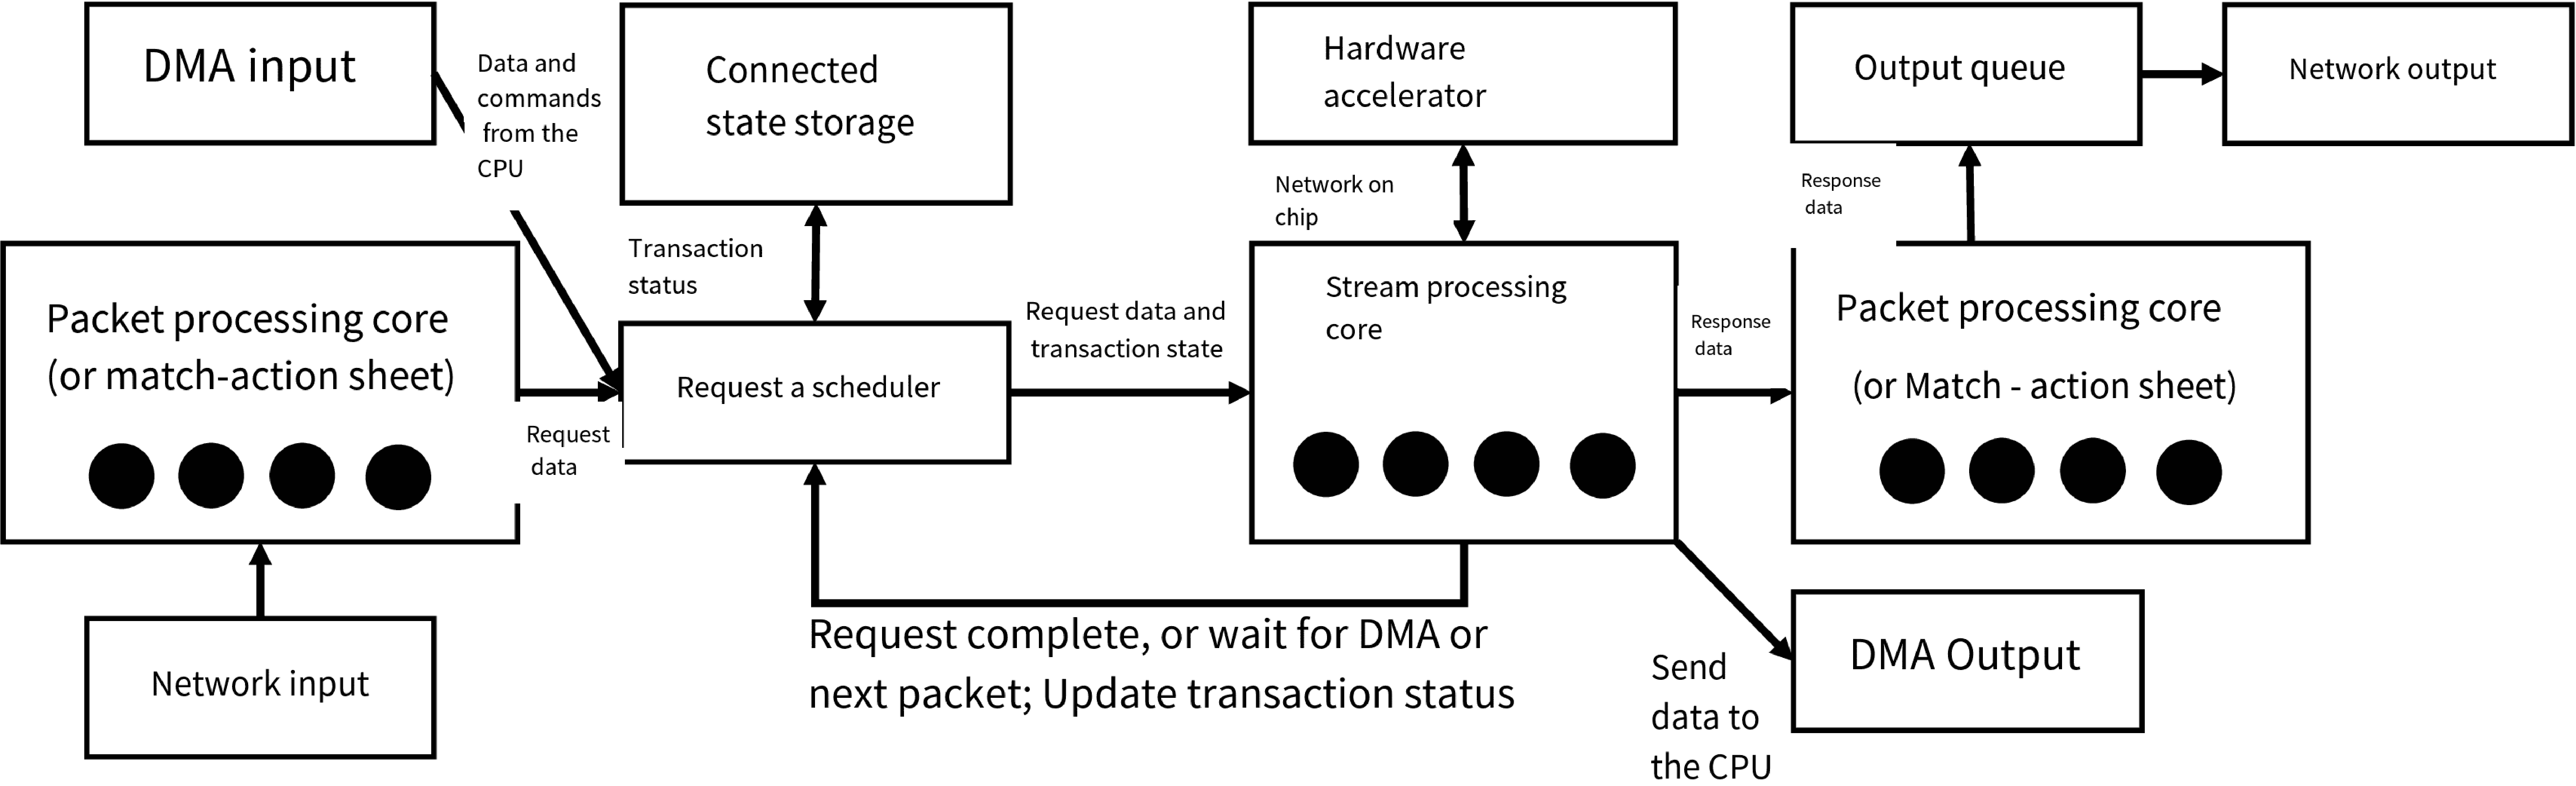
\includegraphics[width=1.0\textwidth]{figures/network_processor.pdf}
	\caption{General architecture of a network processor.}
	\label{background:fig:network_processor}
\end{figure}

Network processors can process network packets and host requests more efficiently than general-purpose processors because they have hardened many packet processing functions into hardware logic. 

Firstly, in terms of Quality of Service (QoS) schedulers, hardware schedulers can implement a centralized First-Come-First-Serve (c-FCFS) scheduling model, while the Receive Side Scaling (RSS) technology of network cards, which dispatches based on connection hash, attempts to simulate a distributed First-Come-First-Serve (d-FCFS) model \cite{kaffes2019shinjuku,ousterhout2019shenango}. In centralized scheduling, the central scheduler maintains a scheduling queue and assigns the head task to the processor that has just completed the previous task. In distributed scheduling, the central scheduler evenly distributes requests to the queues of each processor, and each processor can only process its own queue, so there may be situations where some processor queues are not empty while other processors are idle. Queueing theory shows that c-FCFS has a more balanced load across cores than d-FCFS, and the average delay and tail latency \footnote{Tail latency refers to the highest latency in a set of latency samples. For statistical stability, latency samples are usually sorted from small to large, and then the latency at the 99\%, 99.9\% or other percentile is taken as the tail latency.} are also lower. Moreover, the RSS technology of network cards often cannot accurately simulate the d-FCFS model, because packet processing may be stateful, and in many cases, the same connection needs to be assigned to the same processor core. Only when the number of connections is large and the number of packets per connection is the same, can the d-FCFS model be simulated; but in reality, the number of packets per connection often shows a long-tail distribution, at which point the load on the processor cores is unbalanced. Theoretical analysis \cite{li2017kv} shows that the degree of load imbalance under a long-tail distribution is directly proportional to the number of processor cores. For example, for a network processor with 64 stream processing cores, if the d-FCFS method of allocating connections based on hash is used, the load of the highest-loaded core under a long-tail distribution is 6 times the average core load.

Secondly, many commonly used modules of network processors, such as packet parsing, lookup tables, data structures, timers, DMA engines, etc., are implemented in hardware. If these lookup tables and data structures are implemented in software, they will consume a large number of instructions, affecting data plane processing performance. For example, setting and triggering a timer in software requires about 200 instructions, and parsing a TCP/IP protocol packet requires about 100 instructions \cite{clark1989analysis}. From a latency perspective, in a 1 GHz network processor, if the packet transmission delay needs to be controlled within 1.5 $\mu$s, assuming the PCIe delay is 0.3 $\mu$s and the network data link layer (MAC) delay is 0.2 $\mu$s, and each packet is processed serially within the programmable network card, then the number of instructions for software to process each packet cannot exceed 1000. From a throughput perspective, if line-rate processing of 64-byte small packets under a 40 Gbps network is required, 60 M packets need to be processed per second. Assuming the network processor has 64 processing cores, each core can execute 1 G instructions per second, then the average number of instructions per packet per processing core cannot exceed 1000. Therefore, saving the number of instructions for packet processing is important for both latency and throughput. Network processors greatly alleviate the burden of packet processors and stream processors by implementing common data structures and algorithms in hardware. These hardware modules usually use on-chip network interconnection with the processing cores, allowing the cores to call these modules at any time during processing.

Thirdly, the thread scheduling and context management of the stream processing cores within the network processor are implemented in hardware, so fine-grained latency hiding can be achieved. For example, if a stream processing core calls a DMA operation that takes a long time, or needs to wait for a timer, the hardware will automatically save its context (including registers and the state of the stream being processed), put the thread into the not-ready queue, and switch to the next thread in the ready queue; if the ready queue is empty and the number of concurrent threads has not reached the hardware limit, it can take the next task from the task queue and create a new thread. When the DMA operation returns or the timer is triggered, the thread in the not-ready queue is switched to the ready queue. Most network processors use the non-preemptive cooperative scheduling described above. To support strict priority QoS guarantees and to fully utilize processing capabilities to handle low-priority traffic when high-priority traffic is low, some network processors have preemptive scheduling capabilities. Unlike CPUs on hosts, network processors implement the context management and scheduling functions of the operating system in hardware, greatly reducing the overhead of context switching compared to CPUs. In data center scenarios, the microsecond-level latency hiding of CPU applications has become an increasingly important issue \cite{barroso2017attack}, and the "hardware operating system" design of network processors can also provide some insights for the design of host CPUs.

Fourthly, the memory hierarchy within the network processor is customized, thus the efficiency of memory access surpasses that of general-purpose processors, a feature akin to the architectural advantages of FPGAs. The "memory wall" problem of general-purpose processors is well recognized. If all stream processing cores read and write stream states from shared memory, the overhead of cache consistency is high, which imposes a significant burden on the processor's design. Network processors implement the binding of packet content to packet processing cores and stream state to stream processing cores in hardware, and the packet content and stream state are transported and cached through customized data paths, thereby enhancing memory bandwidth under the same chip area and process.

It is worth noting that although network processors are more energy-efficient than general-purpose processors, they are more challenging to program. Early network processors were typically programmed with microcode of a dedicated instruction set, and due to the absence of a compiler, the abstraction level of the programming language was akin to assembly. Modern network processors generally use general-purpose CPU cores (such as ARM and MIPS) as packet processors and stream processors, hence they can leverage mature compilers and development tool chains, and program in C language. The hardened functions in programmable network cards are invoked in the form of library functions, similar to atomic operations and vector operations on Intel CPUs. Compared with general-purpose processors, the difficulty of programming modern programmable network cards primarily lies in the fact that developers need to invest time in understanding these proprietary library functions and the architecture of the network card, and cannot directly use mature code based on frameworks such as DPDK on general-purpose processors.

In terms of performance, the most significant issue with network processors is that the performance of a single core is low, leading to two implications.
First, stateful streams are often mapped to a single processing core or thread to prevent state fragmentation and out-of-order processing within a single stream. Even though some network processors support dividing stateful processing into multiple stages and processing them in a multi-core pipeline, the number of pipeline stages is constrained by hardware and stream processing logic dependencies.
Therefore, for stateful processing, the packet throughput of a single stream cannot exceed several times the single-core processing capacity of the network processor.
The second implication of low single-core performance is that in order to support higher network bandwidth, the number of processing cores must grow linearly, which not only increases the chip area and power consumption, but also poses challenges to the design of core interconnection, memory hierarchy, and on-chip networks.
At network speeds of 40 Gbps and above, the number of cores increases significantly. The on-chip network and scheduler for dispersing and collecting packets become increasingly complex and inefficient. The entire process of delivering packets to the processing core, processing packets, and then sending them to the network often requires 10 $\mu$s or more of latency.
At this point, the latency is significantly higher than that of dedicated chips, and it exhibits greater variability.

Industry network processor products include Netronome NFP-32xx, Cavium OCTEON, Tilera, Mellanox NP-5, etc. Some of these network processors only have stream processing cores and no packet processing cores, but the overall architecture is similar.

\subsection{General-Purpose Processor (SoC)}
\label{smartnic-soc}

Recognizing the challenges of programming network processors, the industry has proposed a programmable network card architecture based on general-purpose processors. This architecture is akin to the ServerSwitch~\cite{lu2011serverswitch} architecture proposed by Microsoft Asia Research Institute in 2011, comprising a hardware network switch and a general-purpose processor. For instance, the Mellanox BlueField \cite{mellanox-bluefield} programmable network card consists of a Mellanox ConnectX-5 hardware network card and a multi-core ARM processor. The hardware network card is the dedicated chip discussed in section \ref{smartnic-asic}, which implements basic packet parsing, classification, queuing, and forwarding functions. As depicted in Figure \ref{background:fig:smartnic_soc}, the multi-core ARM processor, Mellanox ConnectX-5 traditional network card, and the network card's on-board DRAM are interconnected through a PCIe switch. The PCIe switch further connects to the host CPU, implementing a three-way interconnection between the multi-core processor, traditional hardware network card, and host CPU. The traditional network card communicates with the multi-core ARM processor through the DRAM on the programmable network card board. The hardware network card can communicate with the host CPU and the multi-core ARM processor through the host DRAM. The typical packet reception process is: the traditional network card sends the received packets to the DRAM on the programmable network card board. The multi-core ARM processor retrieves the packets from the DRAM, processes them, and then sends them to the DRAM of the host CPU.

\begin{figure}[htbp]
	\centering
	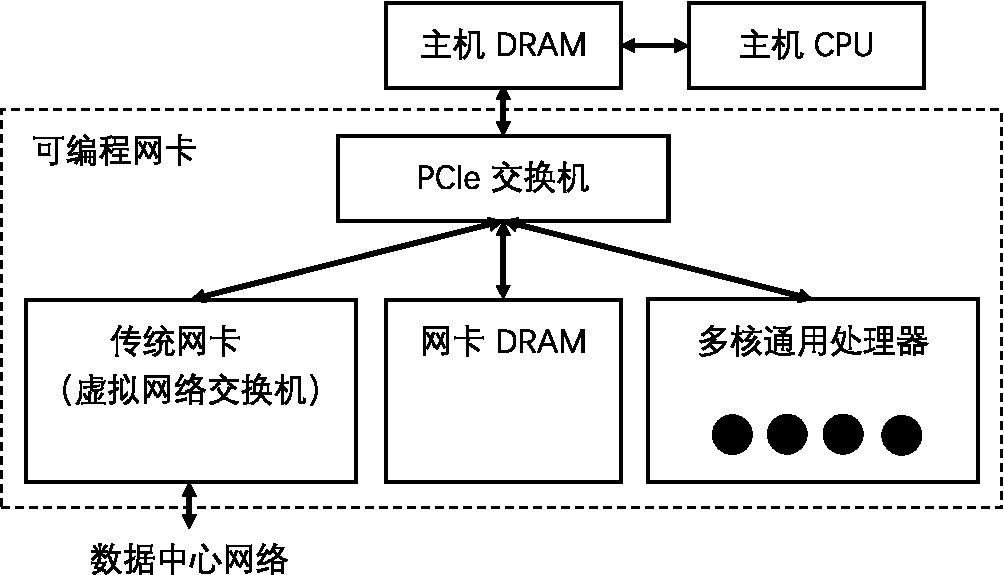
\includegraphics[width=0.7\textwidth]{figures/smartnic_soc.pdf}
	\caption{Architecture of a programmable network card based on a general-purpose processor.}
	\label{background:fig:smartnic_soc}
\end{figure}

Network cards based on multi-core SoCs utilize a large number of embedded CPU cores to process packets, trading off some performance to offer better programmability. The SoC architecture, based on multi-core general-purpose processors, shares many similarities with the network processor (NP) architecture, and is thus often categorized as the same type of architecture. However, they have many differences in reality. Compared to network processors, multi-core SoCs are easier to program, meaning they can adopt standard DPDK code and operate in a familiar Linux environment. Existing network function code based on the host CPU can also be easily cross-compiled to run on multi-core SoCs, while the code of network processors generally needs to be rewritten. Nevertheless, the general-purpose processor cores in multi-core SoCs communicate with traditional network cards using off-chip DRAM, which is less efficient than the access to on-chip high-speed caches in the NP architecture. Table \ref{background:tab:soc-vs-np} compares the SoC and NP architectures of programmable network cards in data centers.

\begin{table}[htbp]
	\centering
	\caption{Comparison of multi-core general-purpose processor and network processor architectures. The numbers come from white papers of programmable network card manufacturers. The actual application performance is affected by the complexity of the application and may not reach the theoretical performance.}
	\small
	\begin{tabular}{l|p{.35\textwidth}|p{.35\textwidth}}
		\hline
		Comparison item & Multi-core general-purpose processor (SoC) & Network processor (NP) \\
		\hline
		\hline
		Instruction type & Standard ARM / MIPS instruction set & Extended ARM / MIPS instruction set \\
		\hline
		Operating system & General-purpose operating system (such as Linux) & No operating system or customized operating system \\
		\hline
		Operating system, paging, etc. & Supported & Generally not supported \\
		\hline
		Context switch and scheduling & Software operating system & Hardware \\
		\hline
		Locks, timers, etc. & Software & Hardware \\
		\hline
		On-board/core communication & Shared memory & Custom data path \\
		\hline
		Packet buffer & Off-chip DRAM & On-chip high-speed cache \\
		\hline
		Packet processing framework & General (such as DPDK) & Dedicated \\
		\hline
		Multi-core queuing model & d-FCFS (hardware dispatch) & c-FCFS (hardware scheduling) \\
		\hline
		Average processing latency & About 5 $\mu$s & Less than 2 $\mu$s \\
		\hline
		Single-core processing capacity & About 3 M pps & About 1 M pps \\
		\hline
		Number of processor cores & About 8 & About 64 \\
		\hline
		Total packet processing capacity & About 24 M pps & About 64 M pps \\
		\hline
		Power consumption & \multicolumn{2}{c}{10 W to 20 W} \\ 
		\hline
	\end{tabular}
	\label{background:tab:soc-vs-np}
\end{table}

As discussed in the preceding section on network processors, both multicore System-on-Chip (SoCs) and network processors are constrained by single-core performance. Although the single-core performance of multicore SoCs surpasses that of network processors, the inter-core communication overhead of multicore SoCs is higher than the hardware pipeline composed of network processor processing cores. Consequently, each packet in multicore SoCs is generally processed to completion on a single processor core (run-to-completion). Therefore, the single-stream performance is typically on the same order of magnitude, around 5 Mpps (packets per second).

In terms of core number increase, since multicore SoCs mostly adopt a distributed first-come-first-serve (d-FCFS) model, if software does not utilize inter-core work stealing techniques, the imbalance of processor load will become increasingly severe with the rise in core number.

In terms of latency, due to the load imbalance among multicore SoC processors, and the non-deterministic latency brought about by the general operating system and general shared memory hierarchy used by multicore SoCs, such as operating system scheduling, interrupts, and cache misses, the latency stability of multicore SoCs is generally poorer than that of network processors, and the tail latency is generally higher than that of network processors.

Therefore, although the multicore SoC method has a familiar programming model and good application compatibility, its evident weaknesses are single-stream performance, higher latency, and poorer scalability at higher network speeds.

From an architectural perspective, multicore SoCs are most similar to host CPUs, as they both use general-purpose processors. However, as shown in Table \ref{background:tab:host-cpu}, whether in terms of cost or performance power consumption, the general-purpose processors used in programmable network cards have clear advantages. In addition, as discussed in Chapter \ref{chapter:intro}, in cloud computing data centers, host CPUs can be sold, and their potential selling price is much higher than the hardware price of a single CPU component. Therefore, using general-purpose processors embedded in programmable network cards in data centers is still advantageous compared to the traditional method of using host CPUs.

The content you provided is already in English and it is in academic style. As per your instructions, I will not make any changes to it.

Intuitively, an FPGA is a large collection of electronic components that can be programmatically reconfigured. These components include logic gates (such as AND, OR, NOT gates), registers, adders, static memory (SRAM), etc., and users can customize their connections to form different circuits. Figure \ref{clicknp:fig:logic-block} illustrates the basic computing unit of an FPGA, which is a logic element composed of programmable logic gates and registers.

\begin{figure}[htbp]
	\centering
	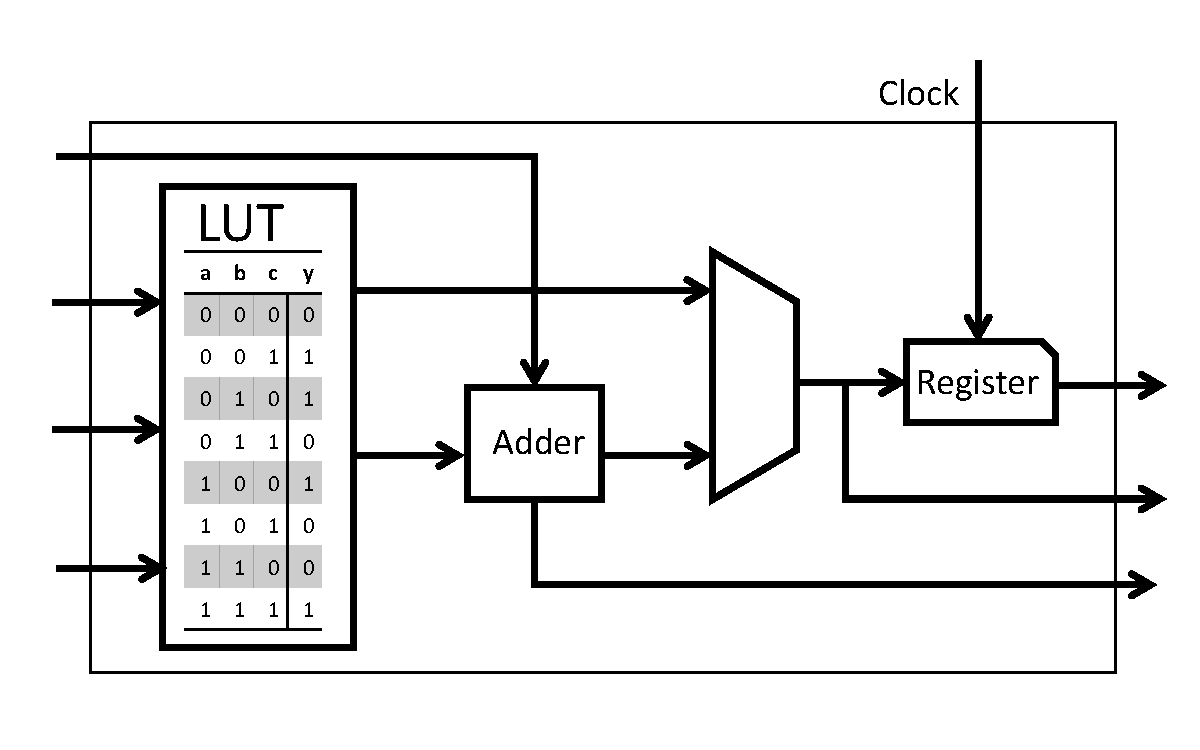
\includegraphics[width=0.7\textwidth]{chapters/clicknp/image/logic-block.pdf}
	\caption{The basic computational unit of FPGA -- logic element.}
	\label{clicknp:fig:logic-block}
\end{figure}

Modern FPGAs, in addition to basic elements, are incorporating an increasing number of DSPs and hard cores (hard IP) to enhance the performance of multiplication, floating-point operations, and access to peripheral devices. The hard cores on the FPGA can support DDR, Ethernet, PCIe, etc., to connect to the on-board DRAM, data center network, host PCIe slot, etc. Figure \ref{clicknp:fig:fpga} presents the logic diagram of the FPGA board used in this paper.

\begin{figure}[htbp]
	\centering
	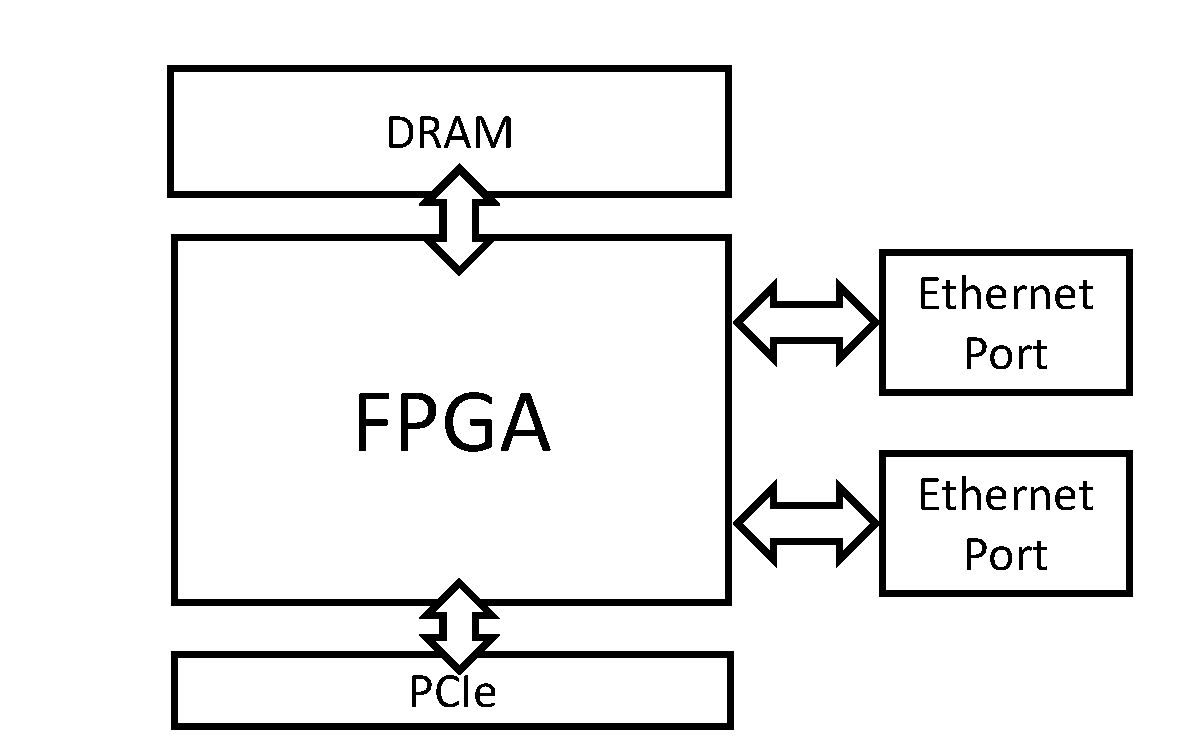
\includegraphics[width=0.6\textwidth]{fpga-board.pdf}
	\caption{Logic diagram of the FPGA board.}
	\label{clicknp:fig:fpga}
\end{figure}

General-purpose processors represented by CPUs usually adopt the von Neumann architecture and its variants. In the von Neumann architecture, since the processor (such as a CPU core) may execute any instruction, it requires an instruction memory, decoder, various instruction operators, and branch jump processing logic. Due to the complexity of the instruction flow control logic, it is impossible to have too many independent instruction flows, so both GPUs and CPUs can use SIMD (Single Instruction Multiple Data) to allow multiple processing units to process different data at the same pace. The function of each logic unit in the FPGA is determined at the time of reprogramming (burning), so no instructions are needed.

In the von Neumann architecture, memory is used for two purposes: saving state and communication between processors. In the von Neumann architecture, all processors share memory, so access arbitration is needed; to take advantage of access locality, each processor has a private cache, which requires maintaining consistency between caches of execution units. For the need to save state, there are a large number of on-chip memory (BRAM) modules in the FPGA, each of which can be connected to the logic module that needs to use the corresponding data, without unnecessary arbitration and cache. For the need for communication between logic modules, the connection between each logic module and the surrounding logic modules in the FPGA has been determined at the time of reprogramming (burning), and there is no need to communicate through shared memory.

%How does the FPGA actually perform? The following will discuss compute-intensive tasks and communication-intensive tasks separately.

%Examples of compute-intensive tasks include matrix operations, image processing, machine learning, compression, asymmetric encryption, Bing search sorting, etc. These tasks are generally offloaded by the CPU to the FPGA for execution. For these tasks, the integer multiplication performance of the Intel Stratix V FPGA is basically equivalent to that of a 20-core CPU, the floating-point multiplication performance is basically equivalent to that of an 8-core CPU, and it is an order of magnitude lower than that of a GPU. The next-generation FPGA, Stratix 10, will be equipped with more multipliers and hardware floating-point computing units, theoretically reaching the computing power comparable to today's top GPU computing cards.

%The latency advantage of the FPGA comes from its architecture.
Because the data path is customized, the FPGA can simultaneously utilize pipeline parallelism \footnote{A pipeline consists of several stages, each task is processed in turn through each stage. There is generally a dependency between the processing of each stage. At any moment, each stage is processing different tasks.}, data parallelism \footnote{In this paper, data parallelism refers to parallel processing of unrelated data, such as vector dot product can use data parallelism, different firewall rules can also be processed in parallel. Note that this is different from the term "data parallelism" in distributed machine learning.} and request parallelism \footnote{In this paper, processing a network packet or an operation offloaded by the host CPU to the accelerator card is called a work request, which is a term in RDMA. Request parallelism refers to the concurrent execution of different work requests. For ease of understanding, the paper often uses data packets instead of work requests.} to reduce latency and increase throughput.
The FPGA can organize a large number of processing units into a computation flow graph according to the dependency of data and control. Those with dependencies are pipeline parallel, and those without dependencies are data parallel. This will be discussed in detail in Chapter \ref{chapter:clicknp}.
The FPGA can also build a scheduler to achieve flexible request parallelism, maintain load balance among processing units, and hide external latency in request processing. This will be discussed in Chapter \ref{chapter:kvdirect}.

The utilization of pipeline parallelism by instruction-based GPUs and CPUs \footnote{In this section, CPU refers to general-purpose processors, including server host CPUs and processors on SoC programmable network cards.} is constrained. Although the instruction processing core is pipelined, its depth is limited; due to the high communication overhead between cores, the efficiency of using multiple cores to form a pipeline is often low.

The parallel computing units of the GPU and the vector instructions of the CPU can exploit data parallelism. However, the data parallelism in both the GPU and the CPU is in the SIMD (Single Instruction Multiple Data) mode, the data being processed in parallel must perform the same operation, and there can be no data dependency between parallel computations. But in many applications, the operations required for different data are different (for example, in firewalls, the packet fields and matching methods matched by different rules are different). If you want to implement data parallelism in SIMD mode, each computing unit needs to traverse all possible operations, thereby wasting some resources for unnecessary operations.
In addition, many operations in packet processing have data or control dependencies, and the speedup that can be obtained by using data parallelism alone is limited. In the FPGA, as long as the data and control dependencies can be determined at compile time, the computation flow graph can be compiled into a pipeline composed of hardware logic.
Finally, many SIMD instructions have restrictions on data alignment and data types, while the FPGA can implement flexible data paths and data types.

Request parallelism cannot reduce the processing latency of a single packet, but it can increase the system's throughput, thereby reducing costs. Both GPUs and CPUs can utilize request parallelism. The computing units within the same group of a GPU can process different packets separately, however, these processing units in the SIMD architecture must follow a unified pace and perform the same operations. Since different packets require different processing operations, as discussed in the data parallelism above, resources need to be wasted to perform unnecessary operations. The computing units in different groups of a GPU can independently process different packets, but the programming model of the GPU usually requires these packets to be input and output together, increasing the input and output latency. Although each core of a CPU can independently receive and send packets from the network card, due to the high communication cost between the CPU and the network card, packets often need to be received and sent in batches to maintain high throughput. When packets arrive one by one instead of in batches, FPGAs can achieve lower latency compared to GPUs and CPUs. In addition, although different cores of a CPU can asynchronously process different packets, load balancing between cores is a challenge. Table \ref{background:tab:fpga-parallelism} summarizes the utilization capabilities of FPGAs, GPUs, and CPUs for pipeline, data, and request parallelism.

\begin{table}[htbp]
	\centering
	\caption{Different architectures' utilization of pipeline, data, and request parallelism.}
	\small
	\begin{tabular}{l|p{.3\textwidth}|p{.25\textwidth}|p{.25\textwidth}}
		\hline
		& Pipeline Parallelism & Data Parallelism & Request Parallelism \\
		\hline
		\hline
		Example & Sequentially processing MAC layer, IP layer, TCP layer, application layer of packets; calculating hash & Matching firewall rules; calculating checksum; vector calculation & Processing different packets; key-value operations \\
		\hline
		FPGA & Can utilize: Custom pipeline & Can utilize: Custom parallel processing units & Can utilize: Custom scheduler \\
		\hline
		GPU & Limited utilization: Instruction processing pipeline, pipeline composed of multiple cores & Limited utilization: SIMD vector operations & Can utilize, but with significant latency issues \\
		\hline
		CPU & Limited utilization: Instruction processing pipeline, pipeline composed of multiple cores & Limited utilization: SIMD vector instructions & Can utilize, but with latency and load balancing issues \\
		\hline
	\end{tabular}
	\label{background:tab:fpga-parallelism}
\end{table}


Therefore, compared to instruction-based processors such as GPUs and CPUs, FPGAs have a latency advantage. For network packet processing, the processing latency of FPGAs can reach microseconds or even nanoseconds. If using a GPU, to fully utilize the computing power of the GPU, the batch size cannot be too small, and the latency will be at the millisecond level, which is more than 1000 times that of the FPGA.\footnote{This is an estimate based on the existing GPU batch processing model network function processing framework. If the GPU supports a streaming processing programming model, its latency will be significantly reduced.} For the host CPU, even using a high-performance packet processing framework like DPDK, the latency is 4 to 5 microseconds, which is an order of magnitude higher than that of the FPGA. A more serious problem is that the latency of the general-purpose CPU is not stable enough. For example, when the load is high, the forwarding latency may rise to tens of microseconds or even higher; the clock interrupt and task scheduling in modern operating systems also increase the uncertainty of latency. In data centers, latency, especially tail latency, is very important. The latency of FPGA processing network packets is at the nanosecond level, and even if it needs to access the host memory through PCIe, it only requires sub-microsecond PCIe latency.\footnote{In the future, after Intel launches Xeon + FPGA connected via QPI, the latency between the CPU and FPGA can be reduced to below 100 nanoseconds, which is on the same order of magnitude as the latency of the CPU accessing the main memory.} In summary, for streaming computing tasks, FPGAs have inherent advantages over GPUs and CPUs in terms of latency.

In terms of delay, the network card receives data packets to the CPU, and the CPU sends them to the network card. Even using a high-performance data packet processing framework like DPDK, the delay is still 4 to 5 microseconds. A more serious problem is that the delay of the general CPU is not stable enough. For example, when the load is high, the forwarding delay may rise to tens of microseconds or even higher; the clock interrupt and task scheduling in modern operating systems also increase the uncertainty of the delay.

Although the GPU can also process data packets with high performance, the GPU does not have a network port, which means that the data packets need to be received by the network card first, and then the GPU is allowed to process them. In this way, the throughput is limited by the CPU and/or network card. Not to mention the latency of the GPU itself.

In summary, the main advantage of FPGA in the data center is its stable and extremely low latency, which is suitable for stream-based compute-intensive tasks and communication-intensive tasks.

FPGA is not a panacea, and there are several technical challenges, as shown in Table \ref{background:tab:fpga-challenges}.

\begin{table}[htbp]
	\centering
	\caption{Challenges of using FPGA as a programmable network card.}
	\small
	\begin{tabular}{l|p{.35\textwidth}|p{.35\textwidth}}
		\hline
		Compared architecture & FPGA challenges & Solutions \\
		\hline
		\hline
		CPU/GPU/NP/SoC & Low clock frequency & Utilize the massive parallelism inside FPGA \\
		\hline 
		CPU/GPU & Low DRAM memory bandwidth & Customize data path, parallel use of on-chip BRAM memory, reduce DRAM usage \\
		\hline
		CPU/GPU/NP/SoC & Hardware description language programming is complex and difficult to debug & Programming framework friendly to software developers based on high-level synthesis technology \\
		\hline
		CPU/GPU/SoC & The software and hardware ecosystem is relatively closed & Open hardware platform, programming framework and IP core \\
		\hline
		CPU/GPU/NP/SoC & The chip area is limited and not suitable for scenarios with complex logic & Separate control plane and data plane; data plane based on customized instructions \\
		\hline
		CPU & High PCIe latency when accessing main memory & Design efficient data structures and use out-of-order execution to achieve latency hiding \\
		\hline
		CPU & Limited PCIe bandwidth when accessing main memory & Design efficient data structures and use on-board cache \\
		\hline
		CPU/GPU/NP/SoC & Need to rewrite for upgrades, interrupt service & FPGA operating system that supports dynamic reconfiguration and seamless service upgrades \\
		\hline
		CPU/NP/SoC & High task switching overhead & Spatial multiplexing, not time-division multiplexing \\
		\hline
		ASIC & Some compute-intensive loads are inefficient & Harden general modules into hard cores \\
		\hline
	\end{tabular}
	\label{background:tab:fpga-challenges}
\end{table}

Firstly, in comparison to CPUs or GPUs, FPGAs typically possess lower clock frequencies and smaller memory bandwidths. For instance, the typical clock frequency of an FPGA is approximately 200MHz, which is an order of magnitude slower than a CPU (2 to 3~GHz). Similarly, the bandwidth of a single on-chip BRAM memory or external DRAM on an FPGA is typically 2 to 10~GBps, while the memory bandwidth of an Intel Xeon CPU is about 60~GBps, and a GPU can reach hundreds of GBps. However, CPUs or GPUs only have a limited number of cores, which restricts parallelism. FPGAs have inherent massive parallelism. Modern FPGAs may have millions of logic units, hundreds of K bits of registers, thousands of on-chip BRAMs (each with a capacity of several MB), and thousands of digital signal processing (DSP) modules. Theoretically, each of these can work in parallel. Therefore, there may be thousands of parallel "\textit{cores}" operating inside an FPGA chip simultaneously. Although the bandwidth of a single BRAM may be limited, if thousands of BRAMs are accessed in parallel, the total memory bandwidth can reach several TBps! Hence, to achieve high performance, programmers must fully utilize this massive parallelism.

Secondly, traditionally, FPGAs are programmed using hardware description languages (HDLs) such as Verilog and VHDL. These languages have a lower level of abstraction, are difficult to learn, and programming is complex. Although high-level hardware description languages like Chisel \cite{bachrach2012chisel} have gained popularity in recent years, they still require programmers to have a basic knowledge of digital logic design and a hardware design mindset. Therefore, the software programmer community has been distant from FPGAs for many years~\cite {bacon2013fpga}. To simplify FPGA programming, the industry and academia have developed numerous high-level synthesis (HLS) tools and systems, attempting to convert programs in high-level languages (mainly C) into HDL. However, they either do not fully utilize the massive parallelism in FPGAs, or have high latency, or are merely a supplement to the hardware development toolchain, and are therefore not suitable for network function processing. A solution to this problem will be proposed in Chapter \ref{chapter:clicknp}.

Thirdly, traditionally, the FPGA hardware developer community has been relatively closed. Firstly, the open-source ecosystem of FPGA is underdeveloped, leading FPGA developers to often need to implement generic modules (IP cores) from scratch or purchase them from third-party vendors. The cost of developing and purchasing generic modules deters many small and medium-sized enterprises and academic researchers. Secondly, the high price of purchasing FPGA boards in small quantities weakens the cost advantage of FPGA compared to other architectures. In recent years, with FPGA becoming a general-purpose accelerator in data centers, FPGA manufacturers and academia have been continuously promoting the construction of the FPGA ecosystem. For instance, the NetFPGA open network programming platform \cite{netfpga}, Xilinx's SDx programming framework \cite{sdaccel}, and the P4 cross-platform network programming language \cite{bosshart2014p4}. Major cloud service providers have also launched on-demand FPGA cloud services and IP core markets, so developers no longer need to spend a high one-time cost to purchase boards and reinvent the wheel. The network element library in Chapter \ref{chapter:clicknp} and the key-value data structure in Chapter \ref{chapter:kvdirect} are beneficial supplements to the FPGA ecosystem.

Fourthly, the logic scale implemented by FPGA with digital circuits is limited by the number of FPGA reconfigurable units, which in turn is limited by the chip area. Therefore, FPGA is not suitable for implementing very complex logic. For complex logic situations, two solutions are generally adopted together.
Firstly, distinguish between the control plane and the data plane, implement the data plane in FPGA, and implement the control plane on a general-purpose processor. For example, Microsoft's virtual network accelerator \cite{smartnic} sends new connections to the control plane on the host CPU, where software determines the processing rules and offloads the rules to the FPGA data plane, so that subsequent packets of this connection can be processed by FPGA. The separation of the control plane and the data plane is a design idea that runs through this article. Compared with programmable network cards using general-purpose processors, using FPGA increases the programming complexity of separating the control plane and the data plane.
Secondly, extract common operations from complex logic and implement customized instructions with digital logic. Complex logic is implemented through a series of customized instructions, which are stored in memory and do not occupy reconfigurable units. Microsoft's virtual network accelerator \cite{smartnic} has designed customized match-operation tables. Microsoft's neural network processor \cite{accelerating-deep-convolutional-neural-networks-using-specialized-hardware} has customized vector processing instructions for neural network calculations. The atomic operations and vector operations in Chapter \ref{chapter:kvdirect} are examples of customized instructions.

Fifthly, to achieve fine-grained cooperative processing between FPGA and CPU, communication via the PCIe bus is necessary. This is because the DRAM capacity on the FPGA board is generally much smaller than the host DRAM, necessitating the storage of large-scale data structures on the host DRAM and access via the PCIe bus. However, the latency of the PCIe bus is in the order of hundreds of nanoseconds, which is an order of magnitude higher than CPU access to main memory. The effective bandwidth of Gen3 x8 is about 6 GB/s, which is an order of magnitude lower than CPU access to main memory. Therefore, accelerated applications on programmable network cards need to design efficient data structures, save memory access times, use out-of-order execution technology to hide latency, and fully utilize the cache of on-chip BRAM and on-board DRAM. This is the theme of Chapter \ref{chapter:kvdirect}.

Sixthly, compared with instruction-based processors, FPGA has a higher task switching overhead. On one hand, although FPGA can achieve data plane task switching without interruption through dynamic reconfiguration, this requires fixing a part of the resources at the physical location on the FPGA chip, which restricts the global optimization of FPGA placement and routing. Additional logic is also needed to assist dynamic reconfiguration, which brings about the area overhead of FPGA.
On the other hand, dynamic reconfiguration of FPGA takes tens of milliseconds, much longer than the time for CPU task switching (CPU task switching based on general-purpose operating systems is generally in the order of microseconds, CPU task switching based on dedicated operating systems is generally in the order of hundreds of nanoseconds, and task switching based on dedicated processors can be completed in tens of nanoseconds). This makes FPGA unable to implement fine-grained time-sharing multiplexing like CPUs. Therefore, the current multi-user multiplexing of FPGA is mainly spatial rather than temporal, similar to allocating different CPU cores to different virtual machines. In addition, during FPGA dynamic reconfiguration, user logic cannot work, so the CPU needs to replace FPGA for processing during this period, or the FPGA service needs to be suspended, which affects the quality of service.
The FPGA programmable network cards discussed in this article are all for the first-party use of data center infrastructure, not for third-party use that is publicly sold, so there is almost no need for dynamic task switching. The main challenge is to use dynamic reconfiguration to achieve service upgrades and to ensure service quality during the upgrade. The author participated in (but did not lead) a project called Feniks \cite{zhang2017feniks} and the recent AmorphOS \cite{khawaja2018sharing} aimed to solve this problem.

Seventhly, some types of workloads are compute-intensive, and their efficiency when implemented in FPGA is significantly lower than that of dedicated chips.
The first type is standardized operations such as encryption and decryption. For example, the RSA asymmetric encryption based on ASIC of the Intel QuickAssist acceleration card \cite{intel-qat} is about 10 times higher in throughput than the FPGA-based implementation in Chapter \ref{chapter:clicknp}.
The second type is common data structures such as lookup tables. For example, Content-Addressable Memory (CAM) is the basis of many concurrent operation schedulers and data structures. CAM can be implemented with tri-state gates in dedicated chips, but its efficiency is lower when implemented in FPGA.
The future work outlook in Section \ref{future:progammable_nic} will propose to learn from the architecture of network processors and harden these operations that are not efficient when implemented in FPGA.

Finally, it should be pointed out that from the perspective of business and supply chain, FPGA has certain disadvantages. The retail price of FPGA is high, and the authorization of the development tool chain is also expensive. Therefore, if the application scale is not large enough, the amortized cost of hardware and tool chain may not be advantageous compared to programmable network cards based on network processors or general-purpose processors. For companies with very large application scales, there are only two main manufacturers of FPGAs for data centers at present, and the supply chain security has a large variable. The secondary development cost of switching between the two FPGAs is high, so self-developed network processors or embedded general-purpose processor chips may be a lower and more controllable choice in the long run. FPGA, as a compromise between general-purpose processors and dedicated chips, is suitable for scenarios with medium application scale and high uncertainty of application scenarios.

\section{Application of Programmable Network Cards in Data Centers}
\label{background:sec:application}

Cloud service providers such as Microsoft Azure, Amazon AWS, Alibaba Cloud, Tencent Cloud, and Huawei Cloud have successively publicized their data center acceleration practices based on programmable network cards.

\subsection{Microsoft Azure Cloud}

At present, Microsoft's primary uses for deploying customized hardware in data centers include computation and infrastructure. In terms of computational acceleration, first, since 2013, it has been used for document selection and sorting algorithms for Bing search \cite{putnam2014reconfigurable}. Since 2016, hardware microservices have been used to consolidate unused resources on multiple FPGAs onto fewer FPGAs, improving FPGA utilization. Second, it is used for compression and encryption algorithms \cite{a-scalable-high-bandwidth-architecture-for-lossless-compression-on-fpgas}, initially only for Bing search, and later extended to Office 365, Cosmos / Azure data lake, Onedrive, cloud storage and other services. Third, since 2015, it has been used for machine learning inference \cite{accelerating-deep-convolutional-neural-networks-using-specialized-hardware,toward-accelerating-deep-learning-scale-using-specialized-hardware-datacenter,serving-dnns-real-time-datacenter-scale-project-brainwave,a-configurable-cloud-scale-dnn-processor-for-real-time-ai}, supporting not only deep learning models but also traditional machine learning models. Fourth, since 2016, it has launched FPGA-supported virtual machine instances, renting FPGA computing power to third-party customers.

The primary uses for infrastructure include networking and persistent storage. In terms of networking, since 2015, it has been used for network virtualization acceleration \cite{smartnic}. For persistent storage, FPGA is used to accelerate Azure cloud storage \cite{calder2011windows}. On one hand, it is used on the storage backend nodes, using the compression and encryption algorithms of the computational acceleration part to improve throughput, adopt better (but more computationally intensive) compression algorithms to improve compression rate, and save storage space; on the other hand, it is used on the storage frontend nodes and computing nodes' storage services, accelerating the data plane of the storage protocol stack through FPGA, realizing data plane bypassing the hypervisor and being able to share storage resources according to the quality of service guarantee.

Considering the above workloads that require acceleration, Microsoft's choice of custom acceleration hardware for data centers is primarily based on three aspects: the architecture of the custom hardware, the connection range between custom hardware, and the communication method between the CPU and the custom hardware.

In terms of custom hardware architecture, FPGA is suitable for both compute-intensive and communication-intensive workloads, and it has low latency. The cost per unit of computing power is lower in large-scale deployment, but the programming complexity is high; GPU is suitable for accelerating compute-intensive workloads, is simpler to program than FPGA, but has higher latency; even in large-scale deployment, the cost per unit of computing power remains high; dedicated ASIC chips are suitable for both compute-intensive and communication-intensive workloads, have the lowest latency, the highest computing power per unit power consumption, but have poor flexibility after functionalization. For instance, the above workloads expanded from Bing search to compression encryption, network, storage, machine learning, deep learning, etc., which is a gradual development process. The design of dedicated chips is difficult to achieve in one step, and redesigning a dedicated chip requires one to two years and tens of millions of dollars in non-recurring engineering costs (NRE).
Based on the above considerations, Microsoft Azure Cloud uses FPGA as the general custom hardware in the data center to accelerate various workloads.

In terms of the communication method between the CPU and the custom hardware, although coherent memory is easy to program, it is not easy to achieve high efficiency on the architecture based on x86 CPU; the bandwidth and latency of network access are relatively limited; Direct Memory Access (DMA) as a standard communication mode on the PCIe bus, becomes the communication method chosen by Microsoft FPGA.
In terms of the connection range between custom hardware, the performance of a single machine is not scalable; the bandwidth of custom interconnects within a rack can be higher, but the cost of adding custom interconnects is high;
Using the existing network interconnection in the data center can achieve the maximum scalability, lower cost, and the bandwidth and latency can meet the needs of most applications.
Historically, Microsoft's FPGA deployment has tried the above three connection methods between custom hardware, which can be roughly divided into three development stages \cite{configurable-cloud-acceleration}:

The content you provided is already in English and in an academic style. As per your instructions, I will not make any changes to it.

\begin{figure}[htbp]
	\centering
	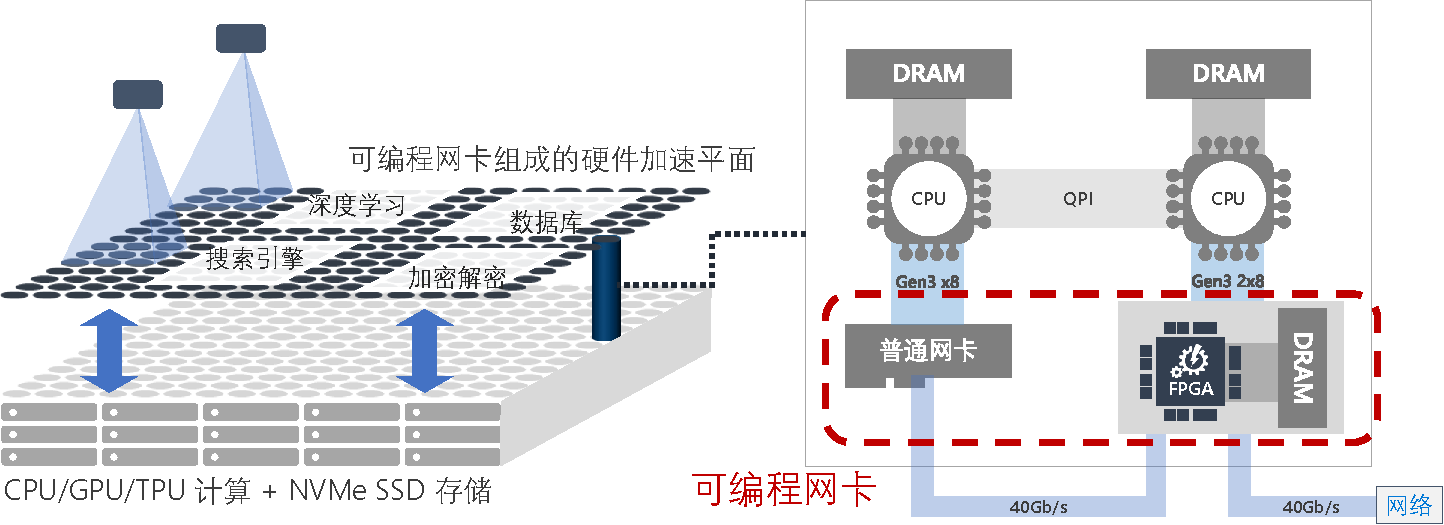
\includegraphics[width=0.8\textwidth]{figures/azure_fpga.pdf}
	\caption{Microsoft's FPGA-based programmable network card.}
	\label{background:fig:azure_fpga}
\end{figure}

This represents Microsoft's third-generation FPGA deployment architecture, and it is also the architecture currently used for large-scale deployment of "one FPGA per server". The original intention of FPGA to reuse the host network is to accelerate the network and storage, and the more far-reaching impact is to extend the network connection between FPGAs to the scale of the entire data center, making it a truly cloud-scale "supercomputer" \cite{configurable-cloud-acceleration}. In the second-generation architecture, the network connection between FPGAs is limited to within the same rack, and it is difficult to scale up the dedicated network interconnection between FPGAs, and the overhead of forwarding through the CPU is too high.

In the third-generation architecture, FPGAs communicate with each other through the Lightweight Transport Layer (LTL) protocol. The latency within the same rack is within 3 microseconds; 1000 FPGAs can be reached within 8 microseconds; all FPGAs in the same data center can be reached within 20 microseconds. Although the second-generation architecture has lower latency within 8 machines, it can only access 48 FPGAs through the network. In order to support a wide range of FPGA communication, the LTL in the third-generation architecture also supports the PFC flow control protocol and the DCQCN congestion control protocol.
FPGAs interconnected through high-bandwidth and low-latency networks form a data center acceleration plane between the network switching layer and traditional server software. In addition to the network and storage virtualization acceleration required by each server providing cloud services, the remaining resources on the FPGA can also be used to accelerate Bing search, deep neural networks (DNN) and other computing tasks.

At the NSDI'18 conference, Microsoft published its practice of using FPGA-based programmable network cards for network virtualization acceleration since 2015 \cite{smartnic}. With the programmable network card, the throughput between Azure virtual machines can reach up to 31 Gbps. During the same period, the network virtualization implementation of Google Cloud Platform (GCP) based on host CPU software \cite{andromeda} could only reach a throughput of 16 Gbps. Amazon AWS's Nitro network virtualization acceleration based on general-purpose processors \cite{nitro-talk} can only reach a throughput of 23 Gbps. Due to the limitation of the single-core performance of the general-purpose processor, the throughput of a single TCP stream of AWS can only reach 10 Gbps, while the single-stream throughput of Microsoft Azure and Google Cloud Platform can reach the peak of the virtual machine. This is consistent with the discussion on the architecture of programmable network cards in Section \ref{smartnic-architecture}.

In terms of delay, using the Linux operating system TCP/IP protocol stack, Microsoft Azure achieved an average inter-VM delay of 10 $\mu$s, while the kernel bypass DPDK \cite{dpdk} can achieve an average delay of 5 $\mu$s. During the same period, the average delay of the Google Cloud Platform was 20 $\mu$s, and the average delay of Amazon AWS was 28 $\mu$s. After using FPGA acceleration, the tail delay of Microsoft Azure is more obvious than the average delay. For example, at the 99.9\% percentile, Azure's delay is 20 $\mu$s, the delay of the Google Cloud Platform based on the host CPU is 75 $\mu$s, and the delay of Amazon AWS based on the programmable network card general processor is 32 $\mu$s. At the 99.99\% percentile, Azure's delay is 25 $\mu$s, while the Google Cloud Platform and Amazon AWS both reach or approach 100 $\mu$s. This is because the delay of hardware pipelining is more controllable than software processing, and in software processing, the latency instability is higher on the host CPU running the customer virtual machine than on the general processor of the programmable network card.

\subsection{Amazon AWS Cloud}

At the Re:Invent conference in December 2017, Amazon AWS Cloud released a computing acceleration architecture called "Nitro" \cite{nitro-blog}. According to the information released by Amazon at the 2017 Re:Invent conference and the 2018 AWS Summit \cite{nitro-talk,nitro-web}, AWS uses custom ASICs to implement various acceleration and security features. Initially, AWS weighed between FPGA and ASIC architectures and decided to adopt the ASIC solution. For this, in January 2015, Amazon acquired ASIC design company Annapurna Labs for more than \$3 billion \cite{annapurna}, which is known for designing system-on-chip (SoC) based on ARM cores.

The development of the Nitro project was phased. Similar to Microsoft Azure, the I/O bottleneck of the virtual machine was first manifested on the virtual network. As early as November 2013, AWS's C3 instances introduced a separate network card to implement enhanced networking, using SR-IOV to allow virtual machines to directly access the network card, bypassing the virtual switch software in the virtual machine monitor. This technology helped Netflix achieve a virtual machine network throughput of 2 million packets per second \cite{netflix-aws}.

In January 2015, Amazon Web Services' (AWS) C4 instances started utilizing hardware-accelerated Elastic Block Storage (EBS). The data of the EBS is stored on the storage node, while the customer's virtual machine operates on the computing node, making this a form of remote storage. For the customer's virtual machine, it appears as a virtual storage device, virtualized by the storage management software in the Xen Dom0 of the virtual machine monitor. C4 instances employ high-performance network cards as opposed to traditional ones to connect to remote EBS, thereby enhancing performance.

In February 2017, AWS's I3 instances introduced NVMe local storage and a dedicated storage virtualization chip. Previously, customer virtual machines had to access local storage via the storage management software in the virtual machine monitor. This was necessary as there could be multiple virtual machines on a single physical server, and each virtual machine could only access its own portion of the storage space, necessitating isolation. For NVMe storage with high latency and throughput, the overhead of storage virtualization software is excessive. To address this, the Nitro chip introduced in the I3 instance implements storage isolation in hardware, allowing NVMe storage to be directly passed to the customer's virtual machine through SR-IOV, achieving a storage performance of 3 million I/O operations per second \cite{aws-local-storage}.

In November 2017, AWS's C5 instances significantly altered the virtualization architecture of the computing node. Firstly, the remote storage in the C4 instances still required software to implement virtualization. This could also be implemented in hardware like I3 local storage, but the interface of block storage is more complex than local storage, making hardware implementation more challenging. Secondly, after the network, remote and local storage have all utilized hardware virtualization, only the interrupt (APIC) function of the data plane and the management function of the control plane remain in the management software of the virtual machine monitor. The management function of the control plane is relatively complex, and it is clearly impractical to use pure digital logic. To offload all virtual networks (VPC), EBS, and virtualization control planes to the accelerator card, the Nitro ASIC adopts a system-on-chip architecture based on the ARM core, thereby maintaining the programmability and flexibility of the data plane, and also offloading the control plane to the accelerator card.

After implementing the Nitro accelerator card, AWS re-engineered a lightweight virtual machine monitor, Nitro, to replace Xen. The control plane, which was initially running on Xen Dom0, was transferred to the Nitro ASIC, allowing customer virtual machines to achieve performance close to that of bare-metal hosts. AWS later introduced bare-metal instances, where customer code runs directly on physical machines, with all storage and network resources provided by the Nitro card.

The Nitro series chips primarily consist of three chips \cite{nitro-blog,nitro-talk,nitro-web}:
\begin{enumerate}
	\item Cloud network (VPC) and elastic block storage (EBS) acceleration chips, which connect the data center network on one side and connect to the CPU in the form of a PCIe card on the other side;
	\item Local NVMe storage virtualization chip, which acts as an intermediary between the CPU and NVMe storage devices;
	\item Security chip, used to verify the version of various device firmware in the server, and to re-flash the firmware to erase traces when switching tenants on bare-metal servers.
\end{enumerate}

The functions of the Nitro chip can be categorized into three aspects: cost reduction, performance improvement, and security enhancement. Let's discuss these in detail.

\textbf{Saving CPU cores.}
Network and storage virtualization require a significant amount of CPU resources to process each network packet and storage I/O request. According to ClickNP \cite{li2016clicknp}, each customer virtual machine's CPU core needs to reserve an additional 0.2 CPU cores to implement virtualization. If these functions can be offloaded to dedicated hardware, the saved CPU cores can be used to install customer virtual machines. Whether considering the price of each CPU core on a public cloud virtual machine or the hardware cost of each core of a Xeon CPU, significant cost savings can be achieved with dedicated hardware \cite{smartnic}.

\textbf{Increasing the maximum number of cores.}
Saving CPU cores can not only reduce costs but also increase the maximum number of cores for large virtual machine instances. Since all major public cloud manufacturers purchase CPUs from the same manufacturers such as Intel, the maximum number of CPU cores that can be purchased at the same time is relatively fixed. After virtualization is offloaded to hardware, all CPU cores are used to run customer virtual machines, so AWS's M5 instance can reach up to 96 CPU cores. If hardware offloading is not used, only 80 CPU cores will be available for customer virtual machines, thereby reducing the attractiveness to customers pursuing extreme performance.

\textbf{Increase single-core frequency.}
Due to power consumption constraints, the number of CPU cores and the average core frequency are inversely related. Under the same generation of CPU architecture, CPUs with higher core frequencies generally have fewer cores. For virtual machine instances with equal core numbers, if traditional software virtualization is used, the physical machine will require 1.2 times the number of CPU cores, which may decrease the average core frequency. For instance, before the launch of the C5 instance, the 72-core EC2 instance had a CPU base frequency of 2.7 GHz, but the C5 instance virtual machine using the same generation Skylake architecture could achieve a CPU base frequency of 3.0 GHz.

\textbf{Improve local storage performance.}
Firstly, on bare metal servers, local NVMe storage can achieve a throughput of up to 400 K IOPS (I/O operations per second) per disk. AWS I3 instances have 8 NVMe SSDs, reaching a throughput of 3 M IOPS. For the common storage virtualization protocol stack, each CPU core can only handle a throughput of about 100 K IOPS, which means that 30 CPU cores need to be occupied to allow the virtual machine to fully utilize the throughput of NVMe storage, which is too costly. Even if there is only one NVMe storage, load balancing among 4 CPU cores is still a problem \cite{li2017kv}. As discussed in section \ref{smartnic-architecture}, because hardware allocation and processing tasks are pipeline-style rather than simple parallelism of multiple processing units, hardware can better guarantee Quality of Service (QoS) than multi-core software.

Secondly, in terms of latency, the average latency of NVMe storage on bare metal servers is about 80 microseconds. Virtualization software not only adds an average latency of 20 microseconds, but also due to the impact of factors such as operating system scheduling, interrupts, cache misses, etc., the tail latency under high load can be as high as 1 millisecond (1000 microseconds). Using hardware offloading can reduce the average latency by 20\%, and reduce the tail latency under high load by more than 90\%.

The text you provided is already in English and in an academic style. As per your instructions, I will not make any changes to it.

\textbf{Enhancing the security of bare metal servers.}
Finally, customer code on bare metal servers can directly access various hardware devices within the server, and may even flash firmware of out-of-band server management (BMC) and other components \cite{bare-metal-security}. If malicious code is embedded in the firmware and activated when the next tenant uses the bare metal server, the consequences are unimaginable. In fact, a large portion of customers choose bare metal servers precisely due to concerns about the isolation of virtual machines. To provide a safe and consistent hardware environment when tenants begin using bare metal servers, the Nitro security chip will overwrite the firmware. Nitro will also perform integrity checks at system startup, which is similar to UEFI trusted boot technology, but the verification scope includes not only the operating system bootloader but also hardware firmware.

\subsection{Alibaba Cloud, Tencent Cloud, Huawei Cloud, Baidu}

In 2018, domestic cloud computing service providers in China actively deployed programmable network cards in data centers. The primary purpose of Alibaba Cloud and Tencent Cloud deploying programmable network cards is to support bare-metal servers. Compared with virtual machines, bare-metal servers can eliminate the overhead brought by virtualization, achieving the highest performance under the same hardware conditions; it is convenient to deploy customers' own virtualization software (such as VMWare); it is completely the same as the deployment environment in the customer's own data center (on-premises), reducing the migration cost of customers to the cloud; it is convenient to use hardware that does not support virtualization or has a significant performance loss after virtualization, such as GPU and RDMA network cards; it does not share server hardware with other tenants, and the isolation and security are stronger, which can also meet some customers' compliance requirements.

The main technical challenge of using bare-metal servers in the public cloud is to access resources such as virtual networks (VPC) and remote storage (EBS) in the data center. A simple method is to place several virtual network and storage servers in the same rack, deploy corresponding software, and configure forwarding rules on the top-of-rack (ToR) switch, so that all network packets of the bare-metal server pass through the virtual network and storage server. This method requires additional server resources, which increases the cost. Another method is to offload the data plane of virtual networks and storage to the top-of-rack switch. However, the programming flexibility of the top-of-rack switch is generally poor \cite{tencent-smartnic}, which is not enough to support application layer protocols of virtual storage and security rules of virtual networks, etc.

Therefore, incorporating a programmable network card into the server has emerged as the most efficient solution to support bare-metal servers. Alibaba and Tencent have adopted the SoC solution that combines the FPGA data plane and the multi-core CPU control plane. In 2018, Alibaba Cloud launched the "X-Dragon" bare-metal server, which uses its self-developed MOC card \cite{alicloud-smartnic,alicloud-xdragon} to achieve network and storage virtualization similar to AWS Nitro. Tencent Cloud unveiled a programmable network card solution based on FPGA at APNet’18, primarily used for network virtualization \cite{tencent-smartnic}. Tencent only required 10 hardware engineers to complete the FPGA logic design in three months, manufacture the programmable network card board in four months, and deploy it within a year \cite{tencent-smartnic}. This is an example of the agile development that can be achieved with FPGA programming. Tencent is broadening the application scope of programmable network cards from bare-metal servers to standard virtual machines, and employs a unified programmable network card architecture for both application scenarios.

Leveraging the technological accumulation of HiSilicon Semiconductor, Huawei has launched two programmable network cards, which are also used to accelerate Huawei Cloud's virtual network. The SD100 series programmable network card \cite{sd100} adopts the SoC architecture based on the multi-core ARM64 CPU, and both the data plane and the control plane operate on the ARM CPU. The IN5500 series programmable network card \cite{in200} employs a network processor (NP) to provide programmability of the data plane, which can achieve a performance of 100 Gbps. With the programmable network card, Huawei Cloud launched the C3ne network-enhanced virtual machine instance, which was the first to achieve packet forwarding at the level of tens of millions per second among domestic cloud manufacturers \cite{huawei-smartnic}.

Although Baidu has not yet launched virtual machine instances accelerated by programmable network cards, it is a pioneer in accelerating compute-intensive applications in data centers with FPGA. As early as 2010, Baidu utilized FPGA for data compression \cite{ouyang2010fpga}. In 2014, Baidu launched the SDA framework for using FPGA for deep learning inference \cite{ouyang2014sda}, and subsequently used FPGA for database SQL processing \cite{baidu-fpga-sql}. In 2017, Baidu proposed the XPU, a full-stack accelerator for data centers based on FPGA, which is used for various computing acceleration scenarios \cite{ouyang2017xpu}.

